\chapter{Simulation Results}\label{ch:06SimulationResults}
\section{Mission control}
\noindent This section briefly describes responsibilities and tasks of mission control module, implementation of mission control module is similar to \emph{LSTS-Neptus} \cite{dias2006mission,dias2005neptus}.

\paragraph{Navigation} main purpose is to execute mission between  ordered waypoint set $\mathscr{WP}$ (\ref{eq:waypointSet}). 

\begin{equation}\label{eq:waypointSet}
    \mathscr{WP}=\left\{W_1,W_2,\dots,W_n:W_i\in\R^3, i\in \left\{1,\dots,n\right\},n\ge 2\right\}
\end{equation}

\noindent Where each waypoint lies in 3D space $\R^3$ and there is at least two waypoints. There is enforcement of implementation condition that distance of any two consecutive waypoints $\forall i,j=i+1,\, \norm{W_i - W_j}\ge r_r$ is greater than reach radius $r_r$. \emph{Goal waypoint} $W_G$ is selected in following manner:
\begin{enumerate}
    \item\emph{First waypoint $W_1\in\mathscr{WP}$} is selected as goal waypoint $W_G$.
    \item\emph{Until last waypoint $W_n\in\mathscr{WP}$} is reached under reach condition $\norm{\vec{x}(t)\to\R^3-W_G}\le r_r$, check reach condition and select next waypoint in ordered set
    \item\emph{When last waypoint $W_n\in\mathscr{WP}$} is reached execute landing sequence. 
\end{enumerate}

\paragraph{Movement execution} of the movement automaton $\mathscr{MA}$ (def. \ref{def:movementAutomaton}). The main functionality of mission control is to link various movement buffers from avoidance grids $\mathscr{A}(t_i)$ into one single movement chain. The overall architecture has been presented in my earlier works \cite{alojzgomola2017}. 

The key concept is as follows. For dynamically generated set of decision times $t_1,$ $t_2,$ $\dots,$ $t_i$ there exists corresponding a set of avoidance grids $\mathscr{A}(t_1),\mathscr{A}(t_2),\dots,\mathscr{A}(t_i)$, where reach sets are given as set of trajectories. Each avoidance grid has corresponding avoidance trajectory which has been selected $\mathscr{T}(\vec{x},B)$. During a flight there exist a corresponding buffer for each decision time $t_1\to B_1, t_2 \to B_2,\dots,t_i\to B_i$. 

Single movement buffer $B_i$ from trajectory $\mathscr{T}(\hat{\vec{x})}(t_i),B_i)$ is given by following equation:
\begin{equation}
    B_i= \left\{m_{i,1},m_{i,2},\dots,m_{i,k},m_{i,k+1},\dots, m_{i,j-1},m_{i,j},\right\},\quad 1 \le k \le i, i \in \N^+
\end{equation}
Where $m_{i,1}$ is first \emph{to be executed/executed} and $m_{i,k}$ is last \emph{to be executed/executed} movement, $m_{i,k+1},\dots,m_{i,j}$ is flushed part (not used part of buffer), $k$ is count of \emph{to be executed/executed movements}, and $i$ is length of movement buffer $B_i$. This can be extended to any buffer belonging to any decision time. Then by assumptions given in \cite{alojzgomola2017}, there exists positive integer $k_i$ for any avoidance grid $\mathscr{A}(t_i)$ such movements can be chained.

\emph{Final movement buffer $B$} (\ref{eq:finalMovementBuffer}) is ordered chain of \emph{to be executed/executed} movements $\left\{m_{a,1},m_{a,2},\dots,m_{a,k}\right\}$ from partial trajectories at times of decision $t_{1},\dots,t_{i}$ with belonging buffers $\{B_1,\dots,B_i\}$.
\begin{equation}\label{eq:finalMovementBuffer}
    B=\bigcup_{B_a=\{B_1,\dots,B_i\}} \left\{m_{a,1},m_{a,2},\dots,m_{a,k}\right\}
\end{equation}
The example of \emph{final movement buffer $B$} is given in fig. \ref{fig:P46ExampleOfMovementBufferChaning}. The blue line represents \emph{to be executed/executed} movements, red line represents \emph{flushed movements}, purple circles represents \emph{decision points} at time $t_1,\dots,t_5$. Last portion at $t_5$ is denominated red, because it was completely throw away due the \emph{waypoint reach condition} was met.
\begin{figure}[H]
    \centering
    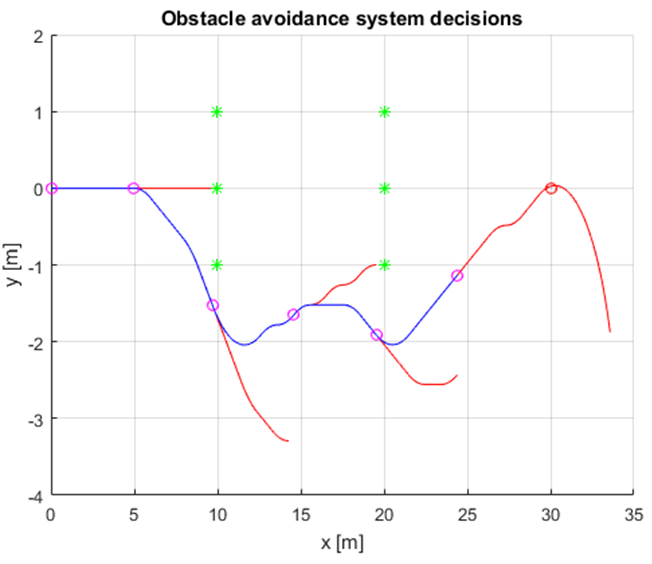
\includegraphics[width=0.7\textwidth]{\FIGDIR/P46ExampleOfMovementBufferChaning}
    \caption{Example of partial movement buffers chaining.}
    \label{fig:P46ExampleOfMovementBufferChaning}
\end{figure}

\paragraph{Obstacle processing and Control switch} has been reused from \cite{alojzgomola2017}.

\section{Reduced reach set approximation computation}
\noindent The worst case scenario for LiDAR scanning have been given in \cite{sabatini2014lidar}. That means the minimal conical range of LiDAR in middle class is $\tilde10$ $m$. The main idea is to test spread reduction vs. coverage ratio $C_R$ on grid with many layers. The deterministic approach of reach set estimation in \cite{alojzgomola2017} was sustainable to calculate full reach set for 5 movements and 10 layers, that implies count of nodes ($n=\sum_{i=1}^10 5^i$). The proposed grid will have 15 layers and 9 movements (estimation of such reach set in full form is impossible). \emph{The pruning of unfeasible pathways} is executed in iterative manner, which enables to minimize memory consumption and effort during \emph{reach set estimation calculation}. The scalability of presented approaches is one of the main features and even the calculation time is scaling well. The approximation algorithm implementation has \emph{borderline polynomial} complexity.


Three different methods have been developed and tested on following avoidance grid $\mathscr{A}(t_i)$:
\begin{enumerate}
    \item Range = 15m, 15 layers
    \item Horizontal range: $\theta\in[-\frac{\pi}{4};\frac{\pi}{4}]$, 7 horizontal cells
    \item Vertical range: $\varphi\in[-\frac{\pi}{6};\frac{\pi}{6}]$, 5 vertical cells
    \item 525 cells, 35 for each layer
\end{enumerate}

\emph{Complexity} of unbounded tree search with pruning procedure after computation is given as:
\begin{equation}
    \mathscr{O}(n) \le m \times r\times h\times v\times l + e^{m \times r} 
\end{equation}
Where $m$ - is count of movements, $r$ is spread rating, $h$ is horizontal cell count of $\mathscr{A}(t_i)$, $v$ is vertical cell count of $\mathscr{A}(t_i)$, $l$ is layer count of $\mathscr{A}(t_i)$. The problematic term is $e^{m \times r}$ which is exponential unexplored nodes residuum. The complexity $\mathscr{O}(n)$ is non-polynomial now. 

To solve this issue the post-expansion pruning algorithm needs to be introduced, this allows to transform $e^{m \times r}$ to a linear/polynomial member $m  \times h \times v \times l$. Therefore complexity $\mathscr{O}(n)$ is now bounded by: 
\begin{equation}
    \mathscr{O}(n) \le m\times (r+1)\times h\times v\times l
\end{equation}
The spread ratio $r$ and movement count $h$ is given, the scalable parameters are grid member counts $h,v,l$, it is obvious that $h\times v \times  l$ is cell count $|\mathscr{A}(t_i)|$. For our grid following formula for boundary can be used:
\begin{equation}
    \mathscr{O}(n) \le 9\times k \times 525
\end{equation}

\noindent The performance parameters for various algorithms are summarized in following table:
\begin{table}[H]
    \centering
    \begin{tabularx}{\textwidth}{l||cccX}
    
    Method/Parameter & Nodes & Trajectories & Coverage ratio $C_R$ & Note\\\hline\hline
    Chaotic method& 2483 & 725 & 0.90 & Forced spread: 9\\
    Harmonic method& 1405 & 180 & 0.30 & \\
    Combined method& 2162 & 305 & 0.87 & CH: 8, H: 1\\
    \end{tabularx} 
    \caption{Reduced reach set computation methods performance}
    \label{tab:RRMethodsPerformanceComparison}
\end{table}

\noindent Reduced reach set approximation $\mathscr{R}_R$ using combined method can cover almost same cell footprints with very small node count:
\begin{equation}
    \frac{\text{node count } \mathscr{R}_R}{\text{node count } \mathscr{R}_F} = \frac{2483}{\sum_{k=1}^{15} 9^k}\sim 1.2088 \times 10^{-12}
\end{equation}
\noindent Depending on selected spread algorithm and pruning algorithm, the reduced reach set keep properties:
\begin{enumerate}
    \item \textit{Smoothness} - trajectories contained in reduced reach set approximation are smooth and with low cost.
    \item \textit{Coverage $C_\mathscr{R}$} - trajectories are covering high amount of footprints from full reach set approximation footprint set $\mathscr{Q}_F$.
\end{enumerate}


\section{Moving obstacles spread models}
\noindent This section discuss implementation and performance of various intruder intersection models. The conditions of intersection was stated as continuous space problem,for real implementation numeric approximation methods keeping probabilistic properties of continuous space were used. 
\noindent Following basic models have been identified in section \ref{sec:intruderIntersectionModel}.:
\begin{enumerate}
    \item \textit{Direct (Line) Intersection} - for static/timed environment.
    \item \textit{Future (Line) Movement} -  for timed environment.
    \item \textit{Vehicle body volume} -  for timed environment.
    \item \textit{Uncertainty spread} -  for static/timed environment.
\end{enumerate}
\noindent Given is intruder $I$ with following properties:
\begin{enumerate}
    \item\textit{Position in Local Coordinate Frame} -  $[6,8,0]^T$
    \item\textit{Velocity} - scalar $1ms^{-1}$, vector $[0,-1,0]^T \quad [ms^{-1},ms^{-1},ms^{-1}]$
    \item\textit{Horizontal spread $\theta$} - $[-\pi/12,\pi/12]\quad [rad,rad]$
    \item\textit{Vehicle body radius} - $2 m$
    \item\textit{Vertical spread $\varphi$} - $[-\pi/16,\pi/16]\quad [rad,rad]$
\end{enumerate}

\noindent All intersection methods have been tested on following avoidance grid $\mathscr{A}(t_i)$:
\begin{enumerate}
    \item Range = 10 m, 10 layers
    \item Horizontal range: $\theta\in[-\frac{\pi}{4};\frac{\pi}{4}]$, 7 horizontal cells
    \item Vertical range: $\varphi\in[-\frac{\pi}{6};\frac{\pi}{6}]$, 5 vertical cells
    \item 350 cells, 35 for each layer
\end{enumerate}

\subsection{Line intersection - Static}
\noindent For line intersection standard \emph{line back-stepping} numeric algorithm was used. Base intersection probability for line $P_T(i_k(\vec{x},\vec{v}),c_{i,j,k})$  (\ref{eq:baseIntersectionProbabilityLineIntersectionType}) was used. The implementation is trivial and intersection probability $P_{O_I}(i_k,c_{i,j,k},l,b,s,\tau)$ (\ref{eq:intruderInCellProbabilityOneIntruder}) The flags are set $l=1$, $b=0$, $s=0$, and $\tau=0$. That means only line intersection is accounted. 
\begin{figure}[H]
    \centering
    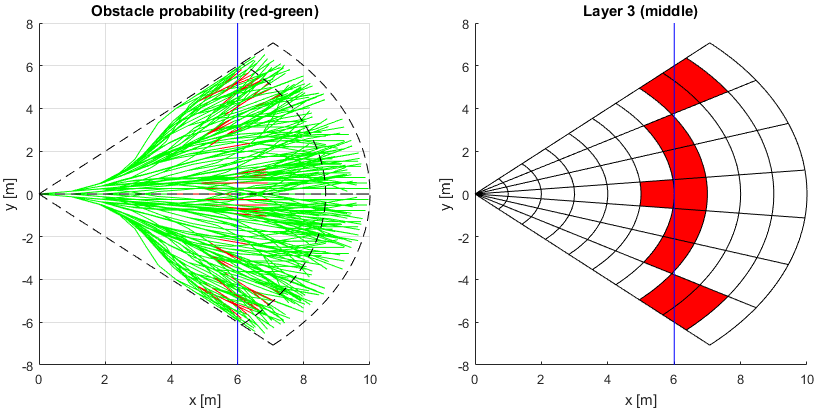
\includegraphics[width=0.7\textwidth]{\FIGDIR/P08LineStaticObstacleSpace}
    \caption{Obstacle space for static line intersection}
    \label{fig:P08LineStaticObstacleSpace}
\end{figure}
\noindent The figure \ref{fig:P08LineStaticObstacleSpace} is showing trajectory space and middle horizontal layer obstacle space $\mathscr{O}(t)$. The blue line is representing intruder intersection trajectory starting at top and finishing at bottom of avoidance grid $\mathscr{A}(t_i)$. The red portion of trajectories on left sub-figure is reflecting the impacted portions of UAV trajectories. The red cells on right sub-figure are reflecting impacted cells with probability of intruder $P_I=1$.
\begin{figure}[H]
    \centering
    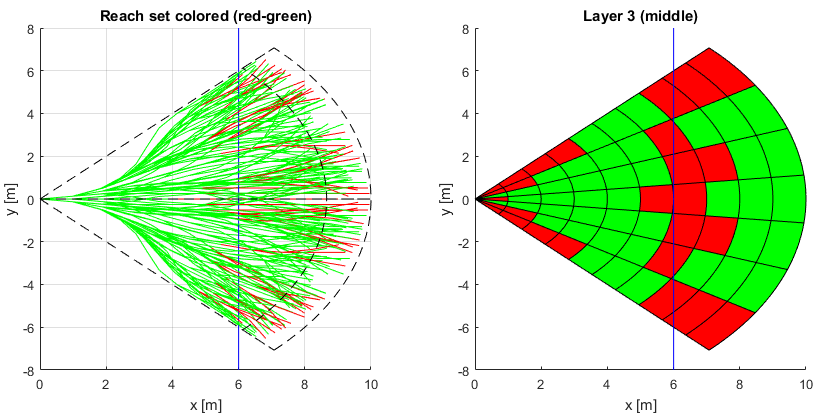
\includegraphics[width=0.7\textwidth]{\FIGDIR/P09LineStaticReachSet}
    \caption{Reach set approximation for static line intersection - middle layer}
    \label{fig:P09LineStaticReachSet}
\end{figure}

\noindent The figure \ref{fig:P09LineStaticReachSet} is showing reachable set approximation trajectories $\mathscr{R}(\hat{x}(t_i),t_i,t_{i+1})$ and middle layer of avoidance grid $\mathscr{A}(t_i)$ with assessed reachability. The blue line is denominating the intruder trajectory (side approach), it starts at top and ends at bottom. The left sub-figure shows set of trajectories where green parts are executable and red parts are crash trajectories. The right sub-figure shows the \emph{reachable space}, the red cells are cells which can not be reached and the green cells are cells which can be reached. Notice that the green cells in front are reachable, because there exists at least one trajectory leading there trough unoccupied space. 

\subsection{Line intersection - Timed}
\noindent For line intersection standard \emph{line back-stepping} numeric algorithm was used. Base intersection probability for line $P_T(i_k(\vec{x},\vec{v}),c_{i,j,k})$  (\ref{eq:baseIntersectionProbabilityLineIntersectionType}) was used. The implementation is trivial and intersection probability $P_{O_I}(i_k,c_{i,j,k},l,b,s,\tau)$ (\ref{eq:intruderInCellProbabilityOneIntruder}) The flags are set $l=1$, $b=0$, $s=0$, and $\tau=1$. That means The base intersection probability and time interval intersection probability components are accounted. The expected danger zones are valid if and only if the intruder and vehicle velocity remains constant. If this condition can not be full-filled the $\tau=0$ in probabilistic model. The obstacle probability is denoted in white/red scale, the reachability probability is denoted in green/red scale.

\begin{figure}[H]
    \centering
    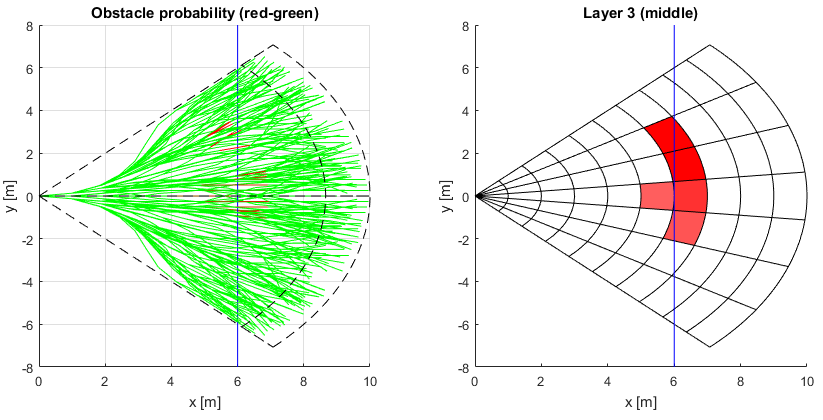
\includegraphics[width=0.7\textwidth]{\FIGDIR/P10LineTimedObstacleSpace}
    \caption{Obstacle space for timed line intersection}
    \label{fig:P10LineTimedObstacleSpace}
\end{figure}

\noindent The figure \ref{fig:P10LineTimedObstacleSpace} is showing trajectory space and middle horizontal layer obstacle space $\mathscr{O}(t)$. The blue line is representing intruder intersection trajectory starting at top and finishing at bottom of avoidance grid $\mathscr{A}(t_i)$. The red portion of trajectories on left sub-figure is reflecting the impacted portions of UAV trajectories. The red cells on right sub-figure are reflecting impacted cells with probability of intruder $P_I\in [0,1]$. Notice that probability of intersection is not always equal to 1, because of time component it can be slightly decreased (pink cells).

\begin{figure}[H]
    \centering
    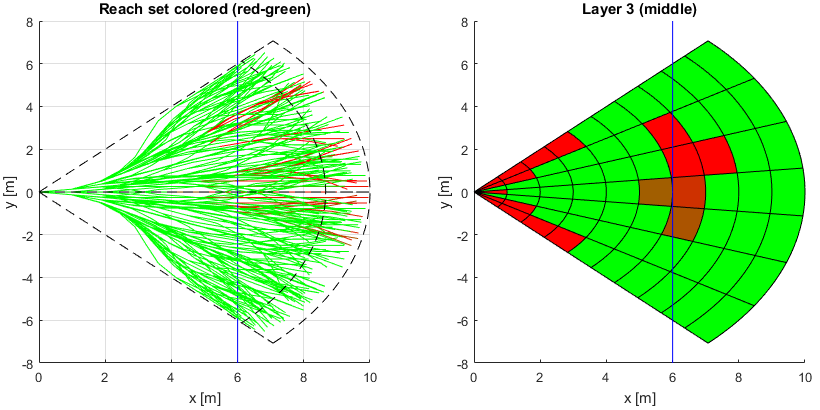
\includegraphics[width=0.7\textwidth]{\FIGDIR/P11LineTimedReachSet}
    \caption{Reach set approximation for timed line intersection - middle layer}
    \label{fig:P11LineTimedReachSet}
\end{figure}


\noindent The figure \ref{fig:P11LineTimedReachSet} shows reachability property intersection with intruder linear trajectory (light blue). The left sub-figure shows the approximation of reach set $\mathscr{R}(\hat{x}(t_i),t_i,t_{i+1})$. The set of trajectories is colored in green-red color, meaning that reachability of the trajectory is absolute when green or not reachable at all if red. The left sub-figure shows reachability status of cells in middle layer. Some of cells are unreachable with reachability probability $P_R(c_{i,j,k})\in [0,1)$. Please note that last layer is fully reachable and intruder can be avoided via the other layers.

\subsection{Line intersection - Future movements}
\noindent For line intersection standard \emph{line back-stepping} numeric algorithm was used. Base intersection probability for line $P_T(i_k(\vec{x},\vec{v}),c_{i,j,k})$  (\ref{eq:baseIntersectionProbabilityLineIntersectionType}) was used. The implementation is trivial and intersection probability $P_{O_I}(i_k,c_{i,j,k},l,b,s,\tau)$ (\ref{eq:intruderInCellProbabilityOneIntruder}) The flags are set $l=1$, $b=0$, $s=0$, and $\tau=1$. That means The base intersection probability and time interval intersection probability components are accounted. The expected danger zones are valid if and only if the intruder and vehicle velocity remains constant. If this condition can not be full-filled the $\tau=0$ in probabilistic model. The obstacle probability is denoted in white/red scale, the reachability probability is denoted in green/red scale. There has been implemented a special case for future movement and it improves time intersection probability:
\begin{equation}
    P_{O_I}(i_k,c_{i,j,k})=
    \begin{cases}
    t_e\ge i_l :& P_{O_I}(i_k,c_{i,j,k},l=1,b=0,s=0,\tau=1)\\
    t_e < i_l  :& P_{O_I}(i_k,c_{i,j,k},l=1,b=0,s=0,\tau=0)/2\\
    \end{cases}
\end{equation}
\noindent Where $t_e$ is vehicle entry time to cell $c_{i,j,k}$, $i_l$ is intruder leave time of cell $c_{i,j,k}$ other notation strictly follows (\ref{eq:intruderInCellProbabilityOneIntruder}). The main idea is to force avoidance from behind of intruder heading, which has been achieved, but is not required to encode higher level decision logic into probabilistic distributions.


\begin{figure}[H]
    \centering
    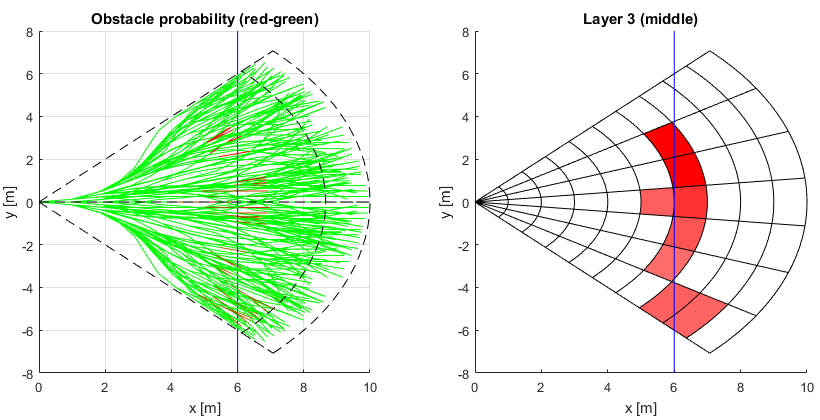
\includegraphics[width=0.7\textwidth]{\FIGDIR/P12LineFutureObstacleSpace}
    \caption{Obstacle space for timed line intersection with future movement}
    \label{fig:P12LineFutureObstacleSpace}
\end{figure}


\noindent The figure \ref{fig:P12LineFutureObstacleSpace} is showing trajectory space and middle horizontal layer obstacle space $\mathscr{O}(t)$. The blue line is representing intruder intersection trajectory starting at top and finishing at bottom of avoidance grid $\mathscr{A}(t_i)$. The red portion of trajectories on left sub-figure is reflecting the impacted portions of UAV trajectories. The red cells on right sub-figure are reflecting impacted cells with probability of intruder $P_I\in [0,1]$. Notice that probability of intersection is not always equal to 1, because of time component it can be slightly decreased (pink cells). The future movement cells are located as new addition at bottom of trajectory, for reference compare fig. \ref{fig:P10LineTimedObstacleSpace}.

\begin{figure}[H]
    \centering
    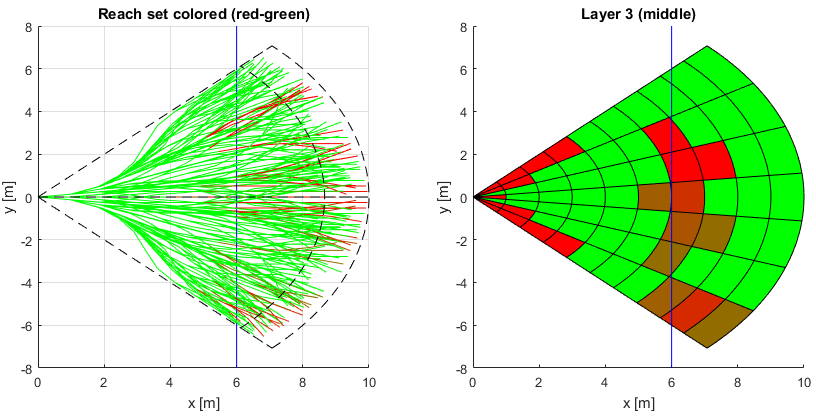
\includegraphics[width=0.7\textwidth]{\FIGDIR/P13LineFutureReachableSpace}
    \caption{Reach set approximation for timed line intersection with future movement - middle layer}
    \label{fig:P13LineFutureReachableSpace}
\end{figure}

\noindent The figure \ref{fig:P13LineFutureReachableSpace} shows reachability property intersection with intruder linear trajectory (light blue). The left sub-figure shows the approximation of reach set $\mathscr{R}(\hat{x}(t_i),t_i,t_{i+1})$. The set of trajectories is colored in green-red color, meaning that reachability of the trajectory is absolute when green or not reachable at all if red. The left sub-figure shows reachability status of cells in middle layer. Some of cells are unreachable with reachability probability $P_R(c_{i,j,k})\in [0,1)$. Please note how reach set have been changed due the future movements, it is almost certain that vehicle will avoid intruder from behind (fig. \ref{fig:P11LineTimedReachSet}).


\subsection{Vehicle body volume - timed}
\noindent\emph{Base intersection probability} $P_T(i_k(\vec{x},\vec{v},r),c_{i,j,k})$ (\ref{eq:baseIntersectionProbabilityBallIntersectionType}) is defined for volume ball $\mathscr{B}(\vec{x}(t),r)$ (\ref{eq:volumeballofIntruder}). The volume ball 
$\mathscr{B}(\vec{x}(t),r)$ is given only as a boundary can be represented as a convex set $S_1$. The grid cell $c_{i,j,k}$ can be represented as polyhedron. The numeric approximation of these two structures intersection was proposed in \cite{deutsch1999best}, \emph{strong conical hull intersection property} guarantees to avoid false positive intersection cases. The algorithm in \cite{deutsch1999best} also gives the volume of the output, which can be used to enhance  \emph{base intersection probability} like follow:

\begin{equation}
    P_T(i_k(\vec{x},\vec{v},r),c_{i,j,k},t)= \frac{V(c_{i,j,k}\cap \mathscr{B}(\vec{x}(t),r))}{V(c_{i,j,k})} \in [0,1]
\end{equation}

\noindent Where $V(c_{i,j,k}\cap \mathscr{B}(\vec{x}(t),r))$ is volume of cell $c_{i,j,k}$ belonging to some avoidance grid $\mathscr{A}(t_i)$ at some avoidance time $t_i$, intersected with a volume of ball $\mathscr{B}$ with center given by $\vec{x}(t)$ (\ref{eq:intruderBasicLinearModel}) and radius $r$. The denominator is simple volume of cell $V(c_{i,j,k})$. The volume of convex polytopes can be calculated with linear complexity $\mathscr{O}(n)$, where $n$ is count of vertexes as proposed in \cite{lawrence1991polytope}.

This is great for fixed time $t$, but the time is not fixed in our case. For fixed time interval $[t_e,t_l]$ where $t_e$ entry time is given as first time when $P_T(i_k(\vec{x},\vec{v},r,t),c_{i,j,k})\neq 0$, and $t_l$ leave time is given as the last time when $P_T(i_k(\vec{x},\vec{v},r,t),c_{i,j,k}) \neq 0$. Then base probability $P_T(i_k(\vec{x},\vec{v},r),c_{i,j,k})$ for varying time $t \in [t_e,t_l]$ can be obtained as a maximum of all probable intersections $P_T(i_k(\vec{x},\vec{v},r),c_{i,j,k},t)$, summarized in following equation:

\begin{equation}
    P_T(i_k(\vec{x},\vec{v},r),c_{i,j,k}) = \max_{t\in [t_e,t_l]} P_T(i_k(\vec{x},\vec{v},r),c_{i,j,k},t)
\end{equation}

\noindent\emph{Tubular intersection} is possible low-cost replacement for embedded, systems, this type of intersection is similar to \emph{conic intersection} (\ref{eq:conicIntersectionCellIntruderDiscrete}), but the vehicle body radius parameter $r_b$ is independent on time. The tubular slice is given as follow: 
\begin{equation}
    \mathscr{T}(\vec{x}(t),\vec{v},r_s,r_b)=\left\{\vec{p}\in\R^3:\forall_{i\neq j} p_i \exists p_j, ||p_i-p_j|| \le r_s, \left(\vec{p} -\vec{x}\right)\perp \vec{v},  \norm{\vec{p}-\vec{x}}\le r_b\right\}
\end{equation}
\noindent\emph{Tubular slice} fox fixed time $t$ and given vehicle position $\vec{x}(t)\in\R^3$ and orientation $\vec{v}\in\R^3$ with defined step radius $r_s$ and defined body radius $r_r$ is given as set of points where each point holds following up to following conditions:
\begin{enumerate}
    \item $\forall_{i\neq j} p_i \exists p_j, ||p_i-p_j|| \le r_s$ - for each point $p_i$ there exists a point $p_j(i \neq j)$ within the step radius $r_s$. This guarantees coverage and homogeneity, the $r_s$ is chosen as 1/10 of average cell $c_{i,j,i,k}\in\mathscr{A}(t_i)$ radius.
    \item $\left(\vec{p} -\vec{x}\right)\perp \vec{v}$ - all points $\vec{p}$ are orthogonal  to velocity vector $\vec{v}$.
    \item $\norm{\vec{p}-\vec{x}}\le r_b$ - all points are within bounded area of circle given by body radius $r_b$.
\end{enumerate}
\noindent The \emph{tube approximation} is given by following equation:
\begin{equation}
    \mathscr{T}(\vec{x},\vec{v},r_s,r_b) = \left\{\bigcup_{\vec{x}(t)=f(\vec{x},\vec{v})}^{t\in[t_s,t_e]} \mathscr{T}(\vec{x}(t),\vec{v},r_s,r_b)\right\}
\end{equation}
\noindent The \emph{tube approximation} is simply union of all tubular slices over defined time period $[t_e,t_l]$ where $t_e$ is entry time and $t_l$ is leave time, mentioned earlier. The interval can be discredited by using steepest function or simple marginalization rule $\norm{\vec{x}(t_i) - \vec{x}(t_{i+1})} \le r_r$. 

If \emph{tube approximation} is used the cell entry $t_e(c_{i,j,k})$ and leave time $t_l(c_{i,j,k})$ are given based on \emph{tubular slices} intersection $\mathscr{T}(\vec{x}(t),\vec{v},r_s,r_b)$ time $t$.

\begin{figure}[H]
    \centering
    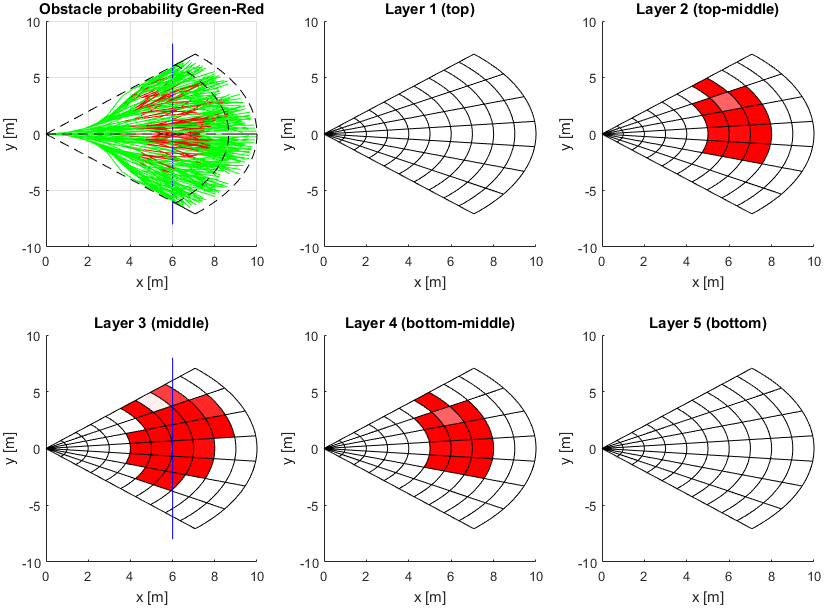
\includegraphics[width=\textwidth]{\FIGDIR/P14VolumeTimedObstacleSpace}
    \caption{Obstacle space for timed intruder body volume}
    \label{fig:P14VolumeTimedObstacleSpace}
\end{figure}
\emph{Obstacle space} for \emph{intruder body volume} with time dependency is depicted in fig. \ref{fig:P14VolumeTimedObstacleSpace} with following meaning:
\begin{enumerate}
    \item\emph{Obstacle probability} - shows how three consequent timed balls $\mathscr{B}(\vec{x}(t),r=1)$ are projected intro reach set approximation $\mathscr{R}(\hat{x}(t_i),t_i,t_{i+1})$, red denotes unfeasible part of trajectories crossing dangerous area where intruder body can be encountered
    \item\emph{Layer 1 (top)} - shows that there is any expectation of intruder body.
    \item\emph{Layer 2} - contains top part of ball intersections, shades of red are denoting intersection probability $[0,1]$, $[white,red]$.
    \item\emph{Layer 3 (middle)} - contains middle part of ball intersections, shades of red are denoting intersection probability $[0,1]$, $[white,red]$. The blue line denotes intruder linear trajectory. 
    \item\emph{Layer 4} - contains bottom part of ball intersections, shades of red are denoting intersection probability $[0,1]$, $[white,red]$.
    \item\emph{Layer 5 (bottom)} - shows that there is any expectation of intruder body.
\end{enumerate}

\begin{figure}[H]
    \centering
    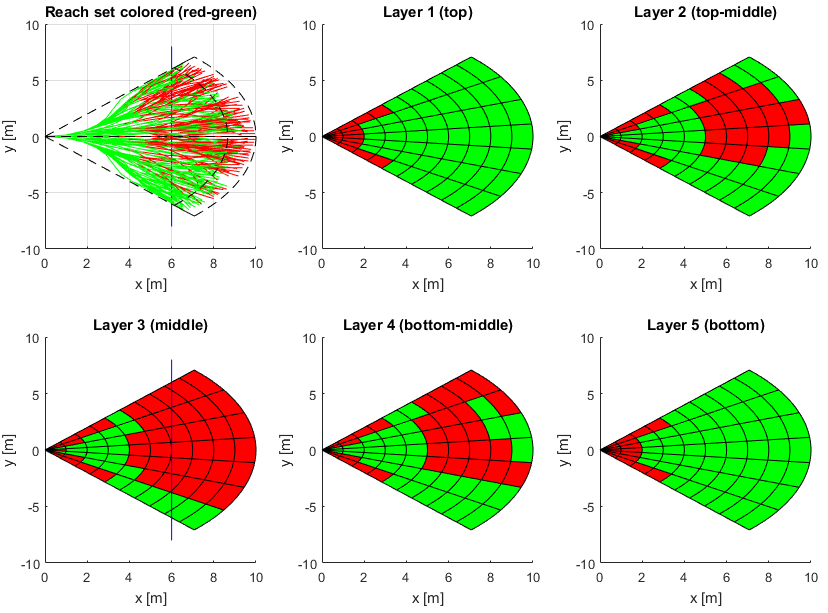
\includegraphics[width=\textwidth]{\FIGDIR/P15VolumeTimedReachSet}
    \caption{Reach set approximation for timed vehicle body volume - all layers}
    \label{fig:P15VolumeTimedReachSet}
\end{figure}

\noindent\emph{Reach set approximation for timed vehicle body volume}  is given by fig. \ref{fig:P15VolumeTimedReachSet}, the explanation of figure is following:
\begin{enumerate}
    \item\emph{Reachability probability} (red-green scale) shows reachability of each point of trajectories contained in reach set approximation $\mathscr{R}(\hat{x}(t_i),t_i,t_{i+1})$, the red shades denotes unreachable parts of trajectories and the green part denotes reachable parts of trajectories.
    \item\emph{Layer 1 (top)} - the top layer is completely reachable.
    \item\emph{Layer 2} - the portion of layer is unreachable, note that some frontal cells are reachable, because there exists trajectories from first layer.
    \item\emph{Layer 3 (middle)} - the middle layer is almost completely unreachable due the intruder occupation of neighbouring layers, intruder trajectory is denoted by blue line.
    \item\emph{Layer 4} - the portion of layer is unreachable due the vehicle body, note that some frontal cells are reachable due the existence of trajectories leading trough fith layer. 
    \item\emph{Layer 5 (bottom)} - the bottom layer is completely reachable
\end{enumerate}

\subsection{Uncertainty spread - Static}
\noindent\emph{Intruder linear model} $\vec{x}(t)=f(\vec{x},\vec{v})$ have been introduced by \ref{eq:vehiclelinearcone}, its simple linear trajectory model, base intersection structure is  \emph{ellipsoid} $E(\vec{x}(t),\vec{v})$ (\ref{eq:baseElipsoidxt}). The \emph{base intersection probability} for single intruder $i_k$ defined as $P_T(i_k(\vec{x}_s,\vec{v},\theta,\varphi),c_{i,j,k})$ is given by \ref{eq:spreadIntruderIntersectionProbDiscrete}. Intruders $i_k$ intersection times for single cell $c_{i,j,k}\in\mathscr{A}(t_i)$ are defined as follow:
\begin{enumerate}
    \item\emph{Intruder time of entry} $i_e(i_k,c_{i,j,k})$ (\ref{eq:conicTimeOfEntryDiscrete}).
    \item\emph{Intruder time of leave} $i_l(i_k,c_{i,j,k})$ (\ref{eq:conicTimeOfLeaveDiscrete}).
\end{enumerate}
\emph{Single Intruder intersection model} $ P_{O_I}(i_k,c_{i,j,k},l,b,s,\tau)$ (\ref{eq:intruderInCellProbabilityOneIntruder}) set up with following flags:  spread flag $s=1$. Because the conical intersection covers a huge amount of space in avoidance grid $\mathscr{A}(t_i)$ it is recommended not to overshoot intruder \emph{horizontal spread} $\theta$ and intruder \emph{vertical spread} $\varphi$ estimates.

\emph{Intruder obstacle probability} $P_{O_I}(c_{i,j,k})$ (\ref{eq:intruderInCellProbability}) was not considered in this simulation, because single intruder was used.  Overall implementation is straightforward transcription of mentioned definitions. 
\begin{figure}[H]
    \centering
    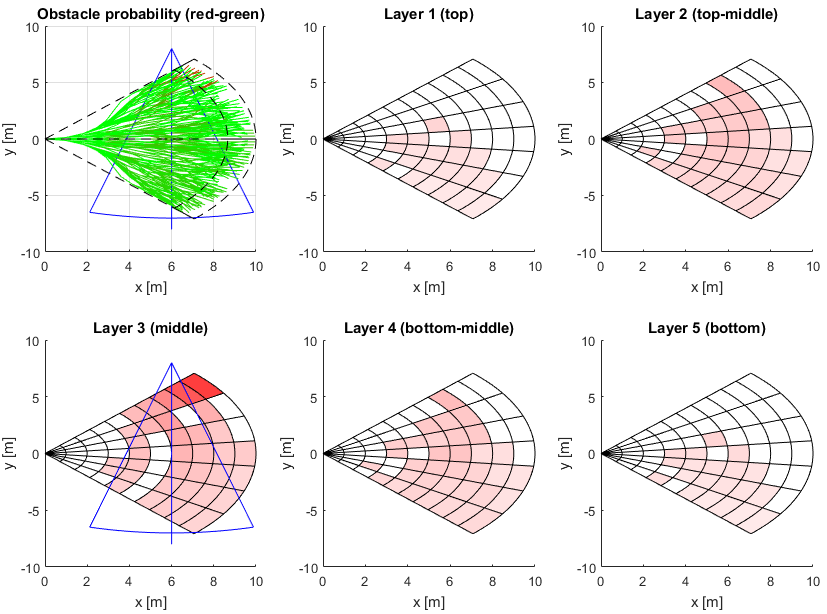
\includegraphics[width=\textwidth]{\FIGDIR/P16SpreadStaticObstacleSpace}
    \caption{Obstacle space for static uncertainty spread}
    \label{fig:P16SpreadStaticObstacleSpace}
\end{figure}

\noindent Uncertainty cone intersection is creating \emph{virtual obstacles}, because real obstacle is moving intruder body. The cone is denoted as \emph{blue} line borders, with notion of vehicle linear trajectory (center axis of cone). Obstacle probability is more concentrated at the detection point (upper part of diagrams) and becomes more spread and thin with increasing horizontal $\theta$ and horizontal $\varphi$ spread. The intruder clash (obstacle) probability distribution is in fig. \ref{fig:P16SpreadStaticObstacleSpace} with following sub-figures:
\begin{enumerate}
    \item\emph{Obstacle probability} - displays impact of intruder on trajectory parts where the intersection with intruder is probable, green denotes low probability, red denotes high probability. The probability is fairly (slightly brownish) low, because of wide spread of intruder horizontal $\theta$, and vertical $\varphi$ distributions.
    \item\emph{Layer 1 (top)} - there is only residual clash probability at the bottom of the diagram, due high vertical spread $\varphi$ value.
    \item\emph{Layer 2} - there is more residual clash probability at the bottom of the diagram, due high vertical spread $\varphi$ value.
    \item\emph{Layer 3 (middle)} - cash probability is concentrated at the top and slowly vanishes over distance from point of detection, due the high horizontal spread $\theta$ value.
    \item\emph{Layer 4} - there is more residual clash probability at the bottom of the diagram, due high vertical spread $\varphi$ value.
    \item\emph{Layer 5 (bottom)} - there is only residual clash probability at the bottom of the diagram, due high vertical spread $\varphi$ value.
\end{enumerate}


\begin{figure}[H]
    \centering
    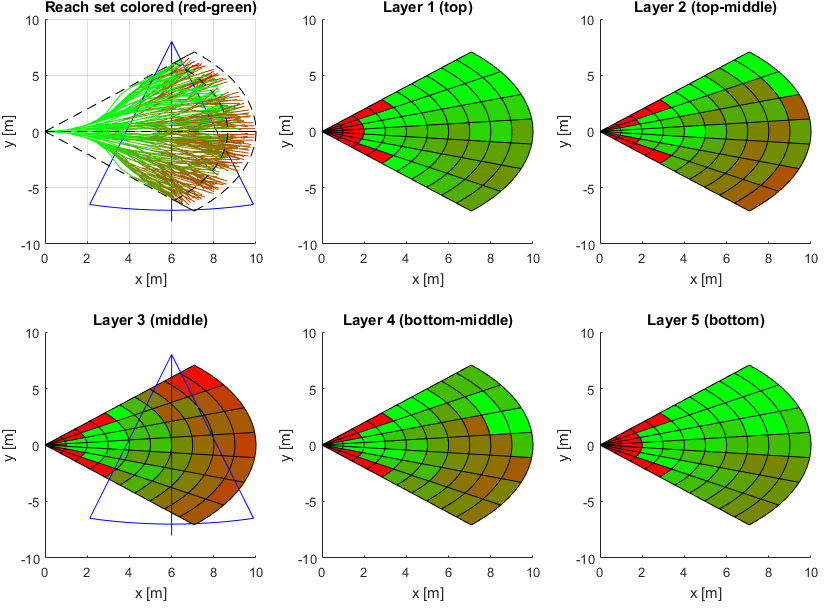
\includegraphics[width=\textwidth]{\FIGDIR/P17SpreadStaticReachSet}
    \caption{Reach set approximation for static uncertainty spread - all layers}
    \label{fig:P17SpreadStaticReachSet}
\end{figure}

\noindent Reach set $\mathscr{R}(\hat{x},t_i,t_{i+1})$(fig. \ref{fig:P17SpreadStaticReachSet}) is given as follow:
\begin{enumerate}
    \item\emph{Reachibility probability} - The reachability probability of trajectories reflects obstacle set $\mathscr{O}(t_i)$
    \item\emph{Layer 1 (top)} - the residual obstacle probability caused from extreme values of \emph{vertical spread} $\varphi$ are causing lowered reachability in lower portions of cells. The upper part is relatively safe.
    \item\emph{Layer 2} - the residual obstacle probability caused from extreme values of \emph{vertical spread} $\varphi$ are causing significantly lowered reachability in lower portions of cells. The upper part is still safe.
    \item\emph{Layer 3 (middle)} - reflects the middle layer in fig. \ref{fig:P16SpreadStaticObstacleSpace}. 
    \item\emph{Layer 4} - the residual obstacle probability caused from extreme values of \emph{vertical spread} $\varphi$ are causing significantly lowered reachability in lower portions of cells. The upper part is still safe.
    \item\emph{Layer 5 (bottom)} - the residual obstacle probability caused from extreme values of \emph{vertical spread} $\varphi$ are causing lowered reachability in lower portions of cells. The upper part is relatively safe.
\end{enumerate}


\subsection{Uncertainty spread - Timed}
\noindent\emph{Intruder linear model} $\vec{x}(t)=f(\vec{x},\vec{v})$ have been introduced by \ref{eq:vehiclelinearcone}, its simple linear trajectory model, base intersection structure is  \emph{ellipsoid} $E(\vec{x}(t),\vec{v})$ (\ref{eq:baseElipsoidxt}). The \emph{base intersection probability} for single intruder $i_k$ defined as $P_T(i_k(\vec{x}_s,\vec{v},\theta,\varphi),c_{i,j,k})$ is given by \ref{eq:spreadIntruderIntersectionProbDiscrete}. Intruders $i_k$ intersection times for single cell $c_{i,j,k}\in\mathscr{A}(t_i)$ are defined as follow:
\begin{enumerate}
    \item\emph{Intruder time of entry} $i_e(i_k,c_{i,j,k})$ (\ref{eq:conicTimeOfEntryDiscrete}).
    \item\emph{Intruder time of leave} $i_l(i_k,c_{i,j,k})$ (\ref{eq:conicTimeOfLeaveDiscrete}).
\end{enumerate}
\emph{Single Intruder intersection model} $ P_{O_I}(i_k,c_{i,j,k},l,b,s,\tau)$ (\ref{eq:intruderInCellProbabilityOneIntruder}) set up with following flags:  spread flag $s=1$, timed $\tau=1$. This settings will intersection cells where is zero chance to meet an intruder with given vehicle dynamics. This option is significantly reducing obstacle space $\mathscr{O}(t_i)$, but if and only if the assumed intruder and vehicle velocities holds static values during collision frame. 

\emph{Intruder obstacle probability} $P_{O_I}(c_{i,j,k})$ (\ref{eq:intruderInCellProbability}) was not considered in this simulation, because single intruder was used. 

\begin{figure}[H]
    \centering
    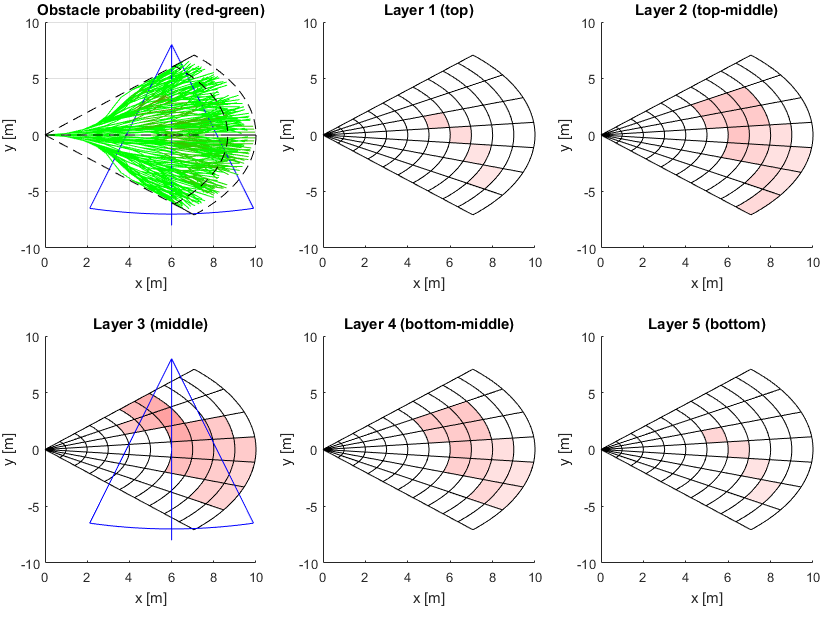
\includegraphics[width=\textwidth]{\FIGDIR/P18SpreadTimedObstacleSpace}
    \caption{Obstacle space for static uncertainty spread}
    \label{fig:P18SpreadTimedObstacleSpace}
\end{figure}
\noindent  Similar to fig. \ref{fig:P16SpreadStaticObstacleSpace} only time aspect is now accounted.

\begin{figure}[H]
    \centering
    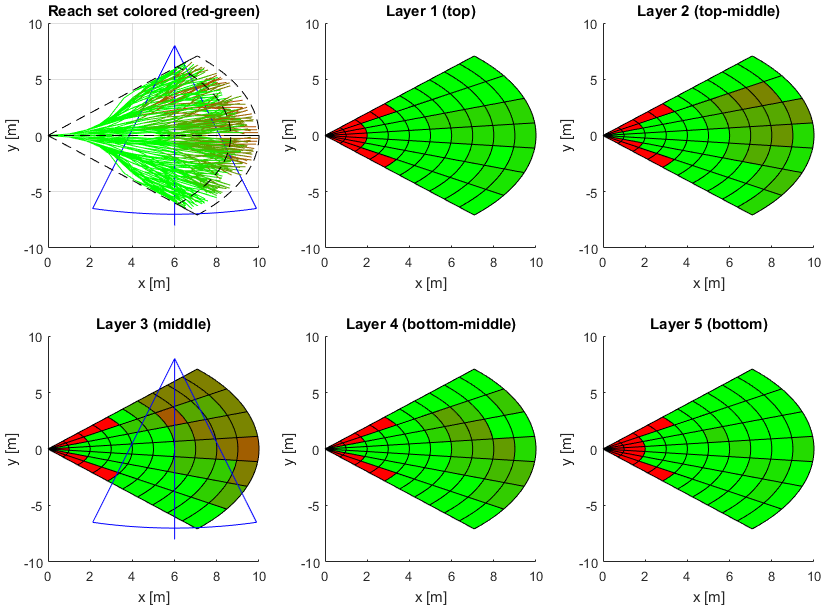
\includegraphics[width=\textwidth]{\FIGDIR/P19SpreadTimedReachSet}
    \caption{Reach set approximation for static uncertainty spread - all layers}
    \label{fig:P19SpreadTimedReachSet}
\end{figure}
\noindent  Similar to fig. \ref{fig:P17SpreadStaticReachSet} only time aspect is now accounted.

\section{Static obstacles avoidance}\label{sec:staticObstacleAvoidanceSimulation}
\noindent \emph{Static obstacle avoidance} testing scenario has been introduced in \cite{alojzgomola2017}. This chapter will introduce only a brief introduction to the test. The vehicle equipped with LiDAR sensor and ADS-B transceiver/receiver is flying in uncharted territory and executing a mission consisting from waypoint set $\mathscr{WP}$. The simulation is executed in mission local coordinate frame, where the vehicle initial position is center of frame and vehicle heading is aligned with main axis.

\noindent The ordered waypoint set $\mathscr{WP}$ is defined as follow:
\begin{enumerate}
    
    \item\emph{Starting waypoint $W_1$} - $[0,0,0]$ - not necessary, just to emphasize the local coordinate frame center
    \item\emph{First obstacle waypoint $W_2$} - $[20,0,0]$.
    \item\emph{Second obstacle waypoint $W_3$} - $[20,20,0]$.
    \item\emph{Third obstacle waypoint $W_4$} - $[0,20,0]$.
    \item\emph{Final waypoint $W_5$} - $[0,0,10]$.
\end{enumerate}

\noindent The obstacle set $\mathscr{O}$ is defined as set of ball obstacles $\mathscr{O}_{\mathscr{B}}(\vec{p},r)$, where $\vec{p}$ indicates obstacle center position and $r$ stands for obstacle radius. The testing obstacle set was defined as follow set of map/detected obstacles $\mathscr{O}_M=\mathscr{O}_D$:
\begin{enumerate}
    \item\emph{First obstacle $\mathscr{B}_\mathscr{O}(1)$} -  $\mathscr{O}_{\mathscr{B}}(\vec{p}=[10,0,0],r=2)$
    \item\emph{Second obstacle $\mathscr{B}_\mathscr{O}(2)$} - $\mathscr{O}_{\mathscr{B}}(\vec{p}=[20,10,0],r=2)$
    \item\emph{Third obstacle $\mathscr{B}_\mathscr{O}(3)$} - 
    $\mathscr{O}_{\mathscr{B}}(\vec{p}=[10,20,0],r=2)$
\end{enumerate}

\noindent Other simulation parameters are stated like follows:
\begin{enumerate}
    \item\emph{Vehicle model $\dot{x}=f(x,u)$} is given by eq. \ref{eq:simple3ddifferentialequations}.
    \item\emph{Vehicle control $\mathscr{MA}$} is defined in section \ref{ch:movementAutomatonPredictor}.
    \item\emph{Vehicle body radius $r_b$} is given as 30 cm.
    \item\emph{Vehicle turning radius $r_t$} is given as 2 m, this parameter impacts the decision time $t_i$ selection based on the in-veritable crash distance \cite{alojzgomola2017}.
    \item\emph{Movement automaton prediction error $E_p=(\mathscr{MA}$)} is equal to 30 cm.
    \item\emph{Safety margin $s_m$} is set to 60 cm.
    \item\emph{Avoidance grid $A(t_i) $}properties were set as follow:
    \begin{enumerate}[a.]
        \item start distance $d_s$ 0 m,
        \item end distance $d_e$ 10 m,
        \item step distance $s_d$ 1 m (10 layers),
        \item horizontal span from $\theta_s$ as $-\pi/4$ to $\theta_e$ to $\pi/4$,
        \item horizontal cell count $c_h$ as $7$,
        \item vertical span from $\varphi_s$ as $-\pi/6$ to $\varphi_e$ to $\pi/6$,
        \item vertical cell count $c_v$ as $5$ (layer count).
    \end{enumerate}
\end{enumerate}

\noindent \emph{Note:} The obstacles are proposed as convex obstacles, the real world obstacles usually breaches the convex surface assumption, the approach was tested on non convex obstacles and open traps. The simplicity of testing example is given to show main properties of approach. Comparison to deterministic approach performance can be made by comparing section 6 of \cite{alojzgomola2017}.

\noindent Legend of simulation results is following:
\begin{enumerate}
    \item\emph{Executed trajectory} (blue line) - executed trajectory by vehicle at moment of snapshot
    \item\emph{Planned trajectory} (red line) - planned trajectory within avoidance grid $\mathscr{A}(t_i)$, trajectory is re-planned every decision time $t_i$. Note that in case of this simulation the trajectory was re-planned every movement.
    \item\emph{Waypoints} (green square markers) - mission plan for multiple waypoints. 
    \item\emph{Obstacles} (red point clouds) - obstacle sets break into point clouds.
    \item\emph{Field of vision} (black dashed line) - denotes current avoidance grid $\mathscr{A}(t_i)$ boundary starting at vehicle position at time of snapshot.
\end{enumerate}
    
\noindent Following decisive moment have been taken into consideration when making snapshots:
\begin{enumerate}
    \item\emph{First obstacle set $\mathscr{B}_\mathscr{O}(1)$ avoidance} (fig. \ref{fig:P31FirstObstacleAvoidance}) - vehicle is heading straight to the obstacle center, the moment captured is when vehicle is avoiding the obstacle. The obstacle is fully covered by field of the vision and vehicle is avoiding it from right side without breaching the safety margin $s_m$. 
    \item\emph{Second obstacle set $\mathscr{B}_\mathscr{O}(2)$ avoidance} (fig. \ref{fig:P35SecondObstacleAvoidance}) - The vehicle is avoiding the second obstacle after the turn, the obstacle is partially in vehicles FOV. The vehicle will crash if there was not a movement restriction given by restriction of reachability property $P_{R}(c_{i,j,k}), \forall c_{i,j,k}\in\mathscr{A}(t_i)$
    \item\emph{Third obstacle set $\mathscr{B}_\mathscr{O}(3)$ avoidance} (fig. \ref{fig:P36ThirdObstacleAvoidance}). - Same as second obstacle. Please note that the cost function $J^*(\mathscr{T}(\vec{x}_0,B))$ is designed to prioritize planar movements. The horizontal/vertical separation was not used in this framework and cost can impact the decision making. 
    \item\emph{Vehicle trajectory after mission competition} (fig. \ref{fig:P37FullAvodanceStaticObstacle}) - The overview of trajectory and decisions, it is assumed that all paths between $W_4$ and $W_5$ are not obscured, this is to show, that avoidance grid $\mathscr{A}(t_i)$ can generate smooth trajectories in free space.
\end{enumerate}

\begin{figure}[H]
    \centering
    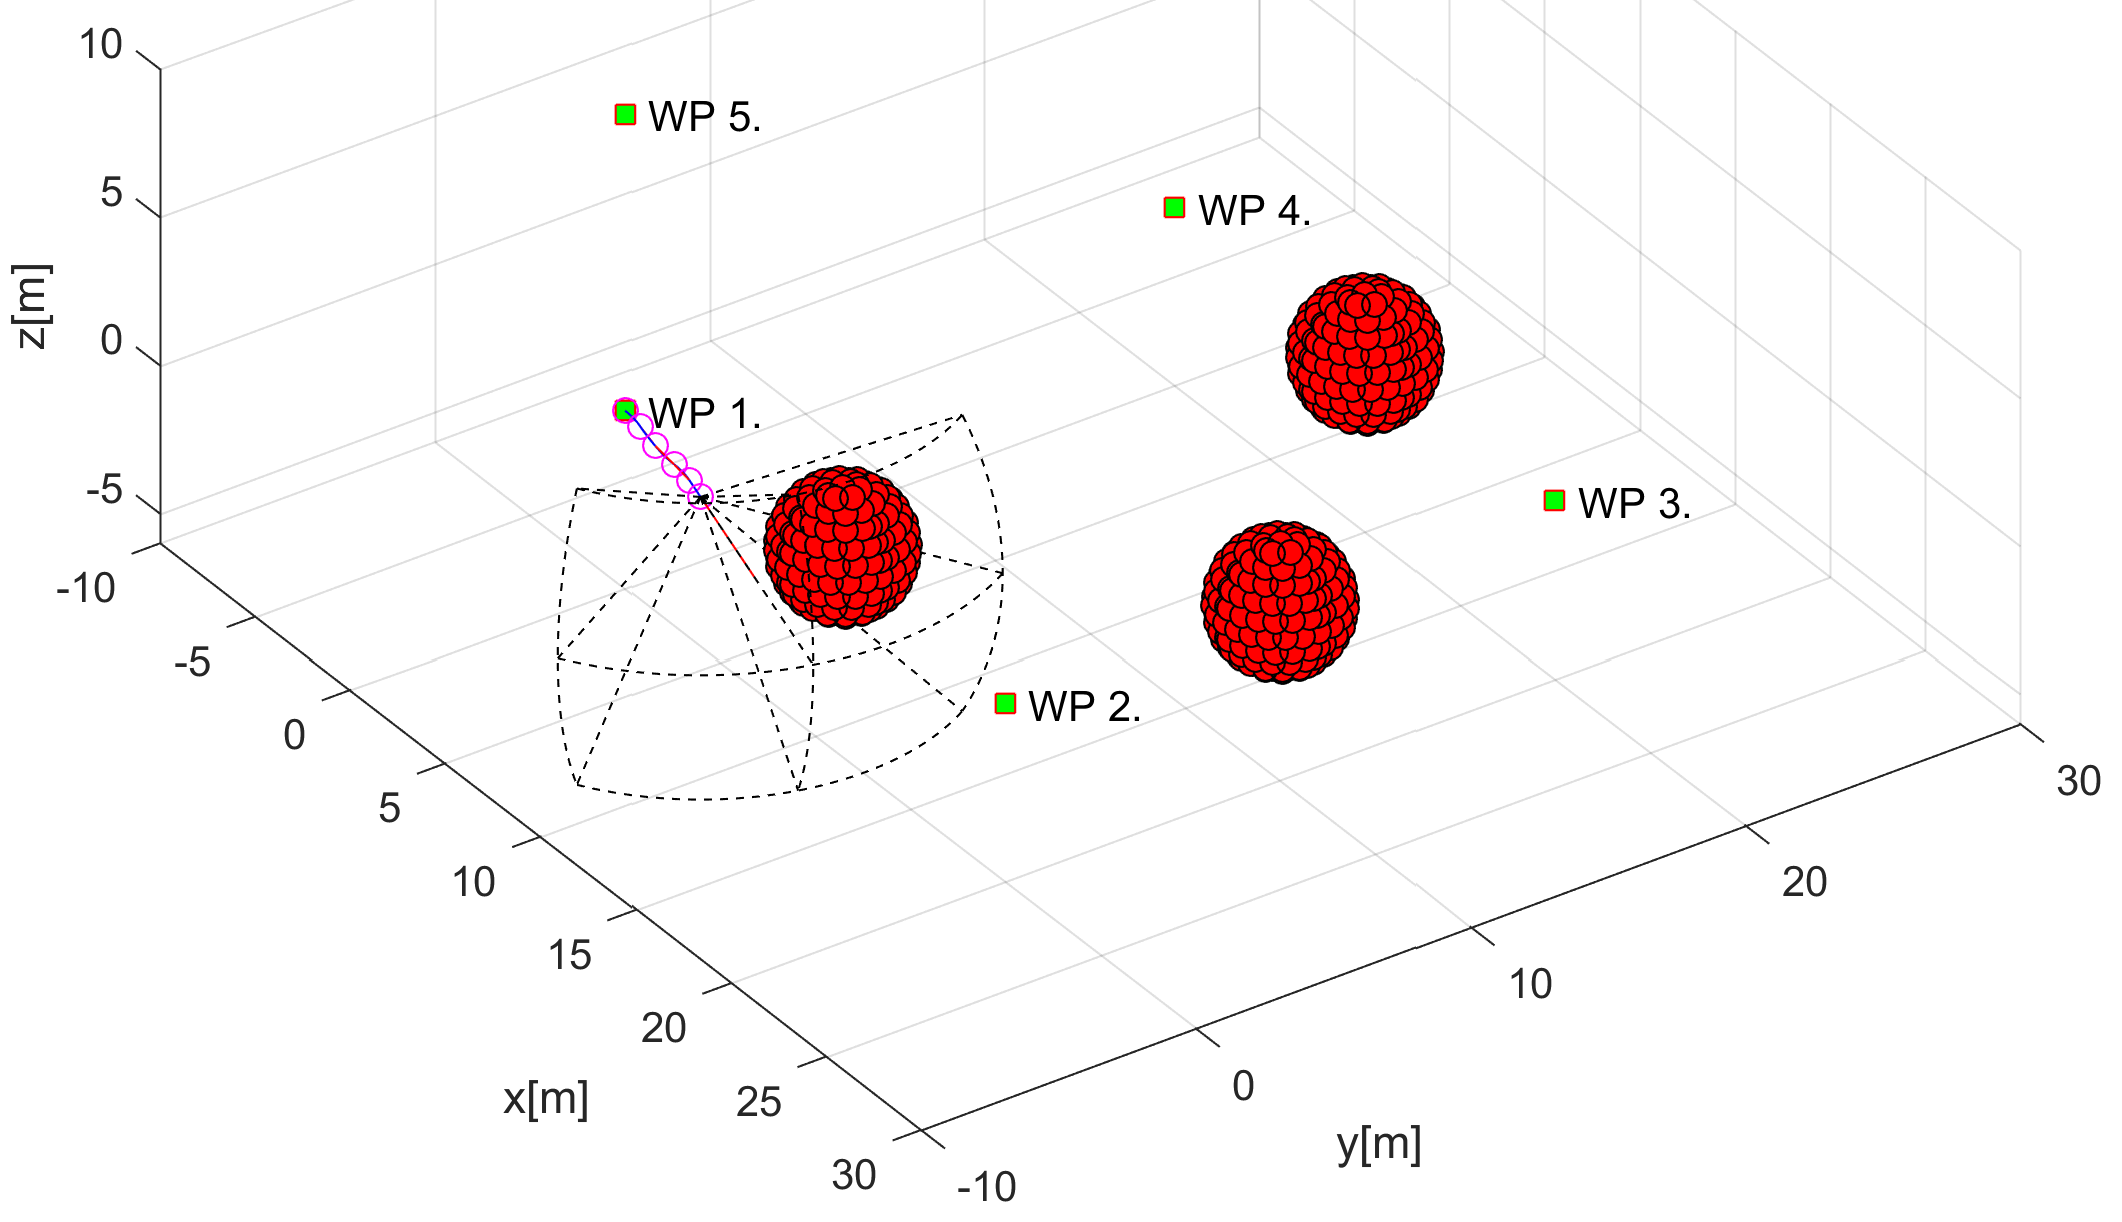
\includegraphics[width=\textwidth]{\FIGDIR/P31FirstObstacleAvoidance}
    \caption{First obstacle set $\mathscr{B}_\mathscr{O}(1)$ avoidance}
    \label{fig:P31FirstObstacleAvoidance}
\end{figure}

\begin{figure}[H]
    \centering
    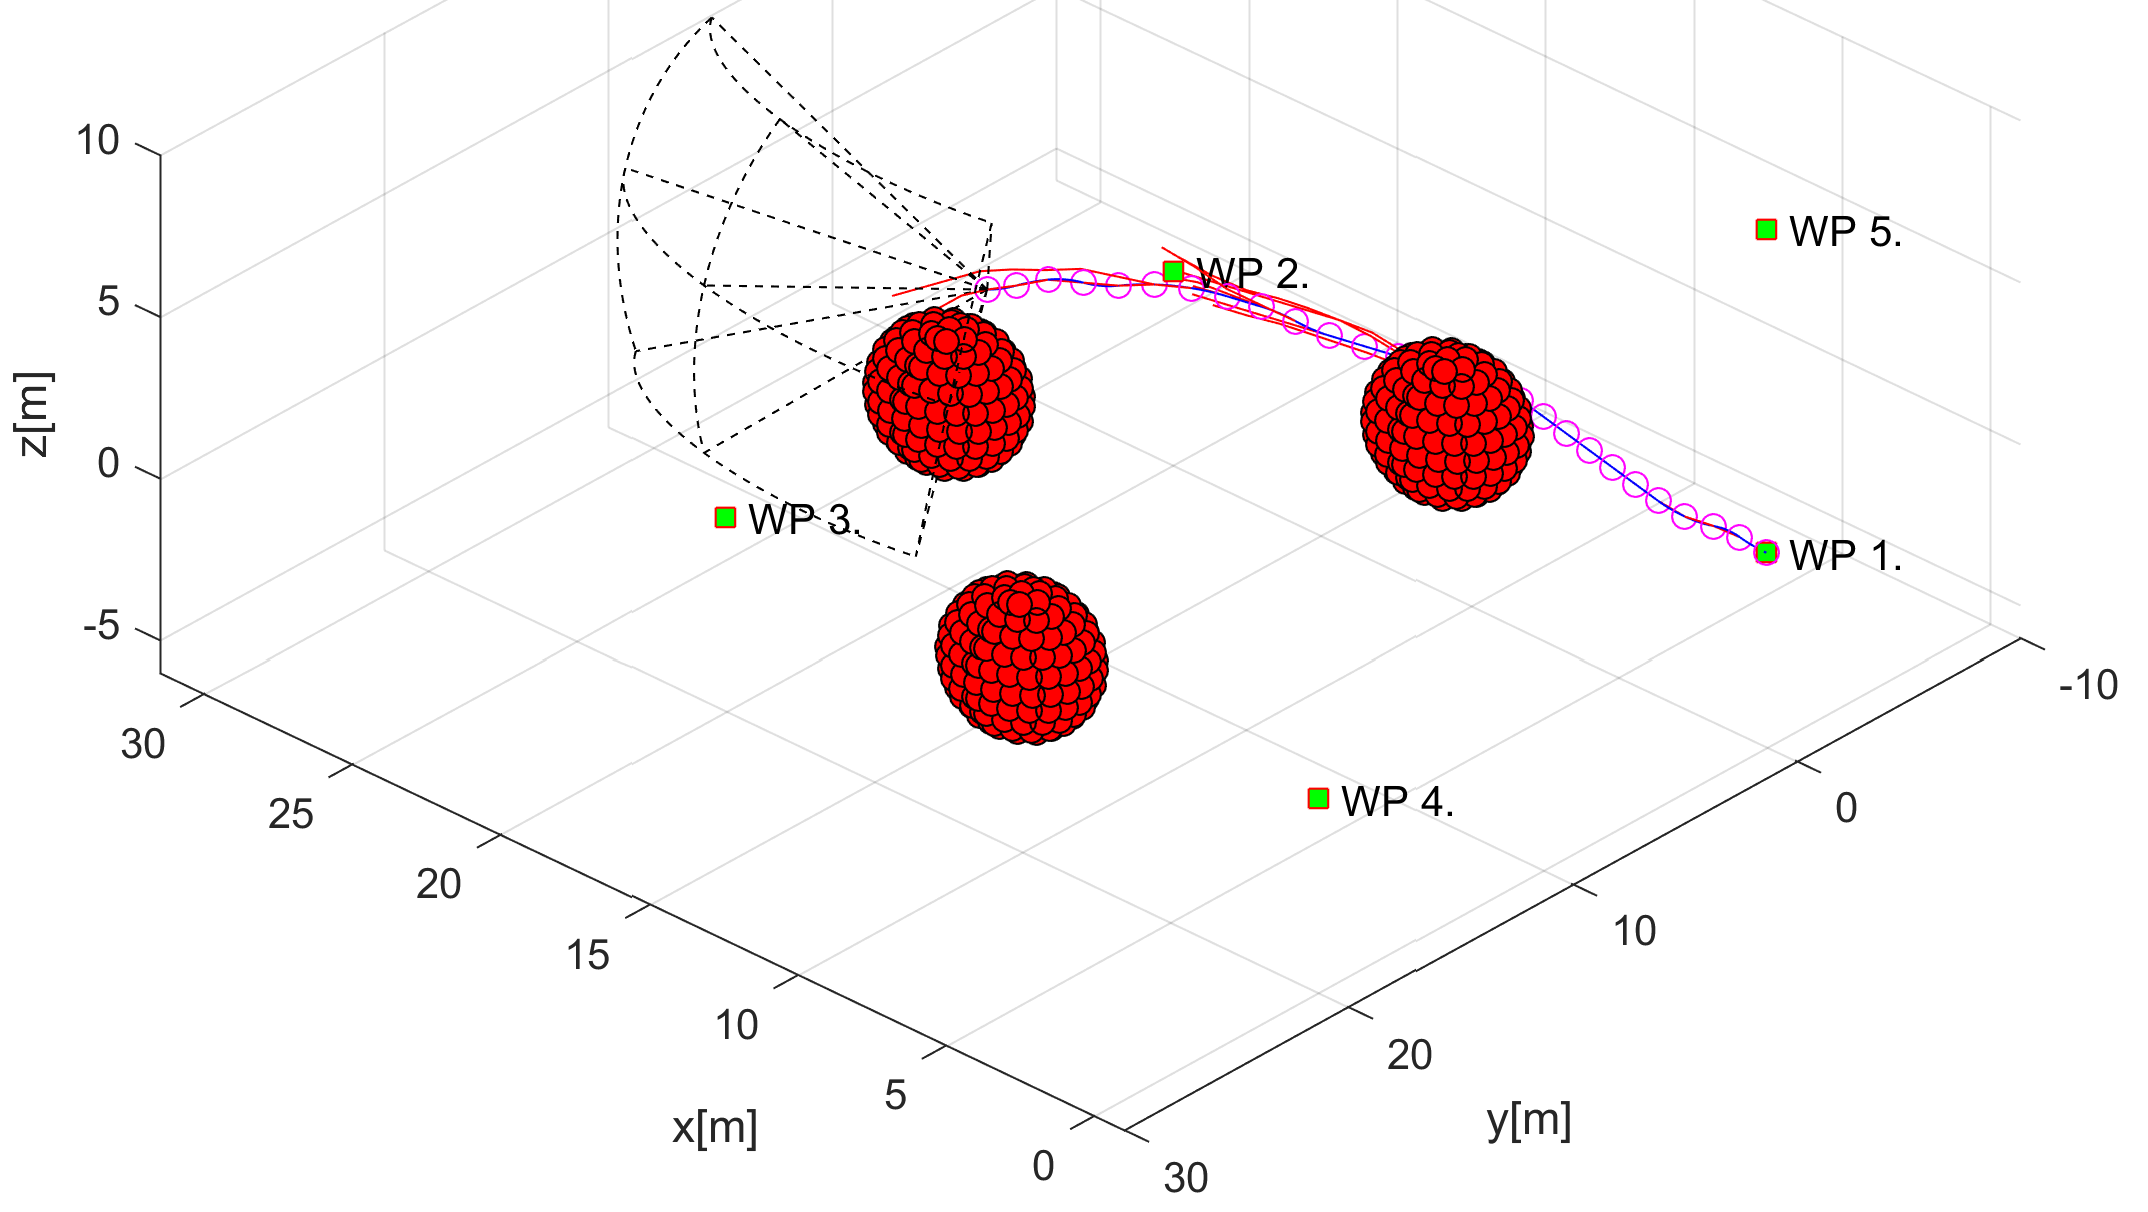
\includegraphics[width=\textwidth]{\FIGDIR/P35SecondObstacleAvoidance}
    \caption{Second obstacle set $\mathscr{B}_\mathscr{O}(2)$ avoidance}
    \label{fig:P35SecondObstacleAvoidance}
\end{figure}

\begin{figure}[H]
    \centering
    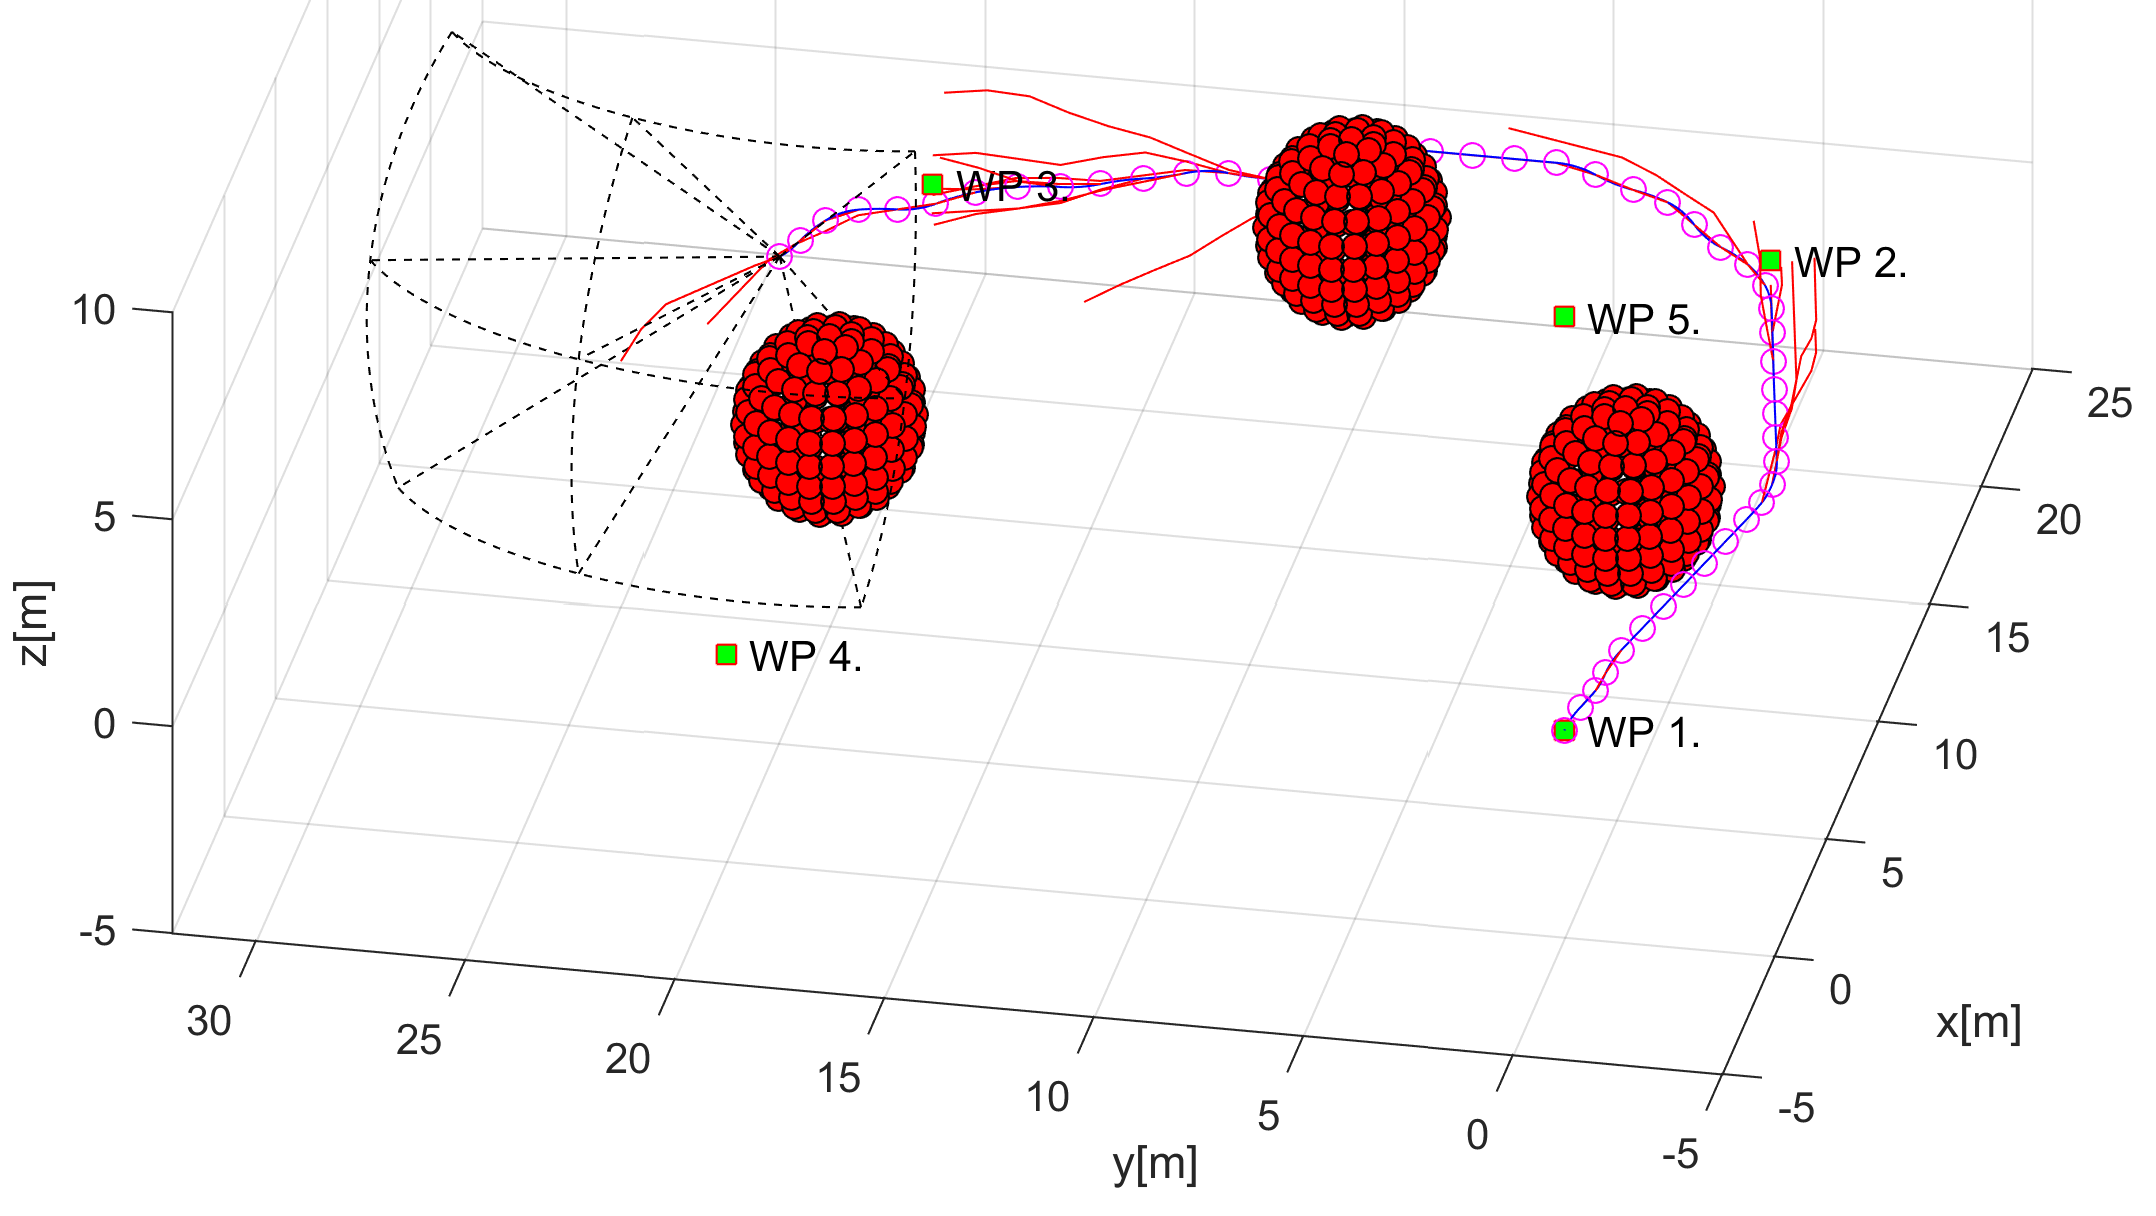
\includegraphics[width=\textwidth]{\FIGDIR/P36ThirdObstacleAvoidance}
    \caption{Third obstacle set $\mathscr{B}_\mathscr{O}(3)$ avoidance}
    \label{fig:P36ThirdObstacleAvoidance}
\end{figure}

\begin{figure}[H]
    \centering
    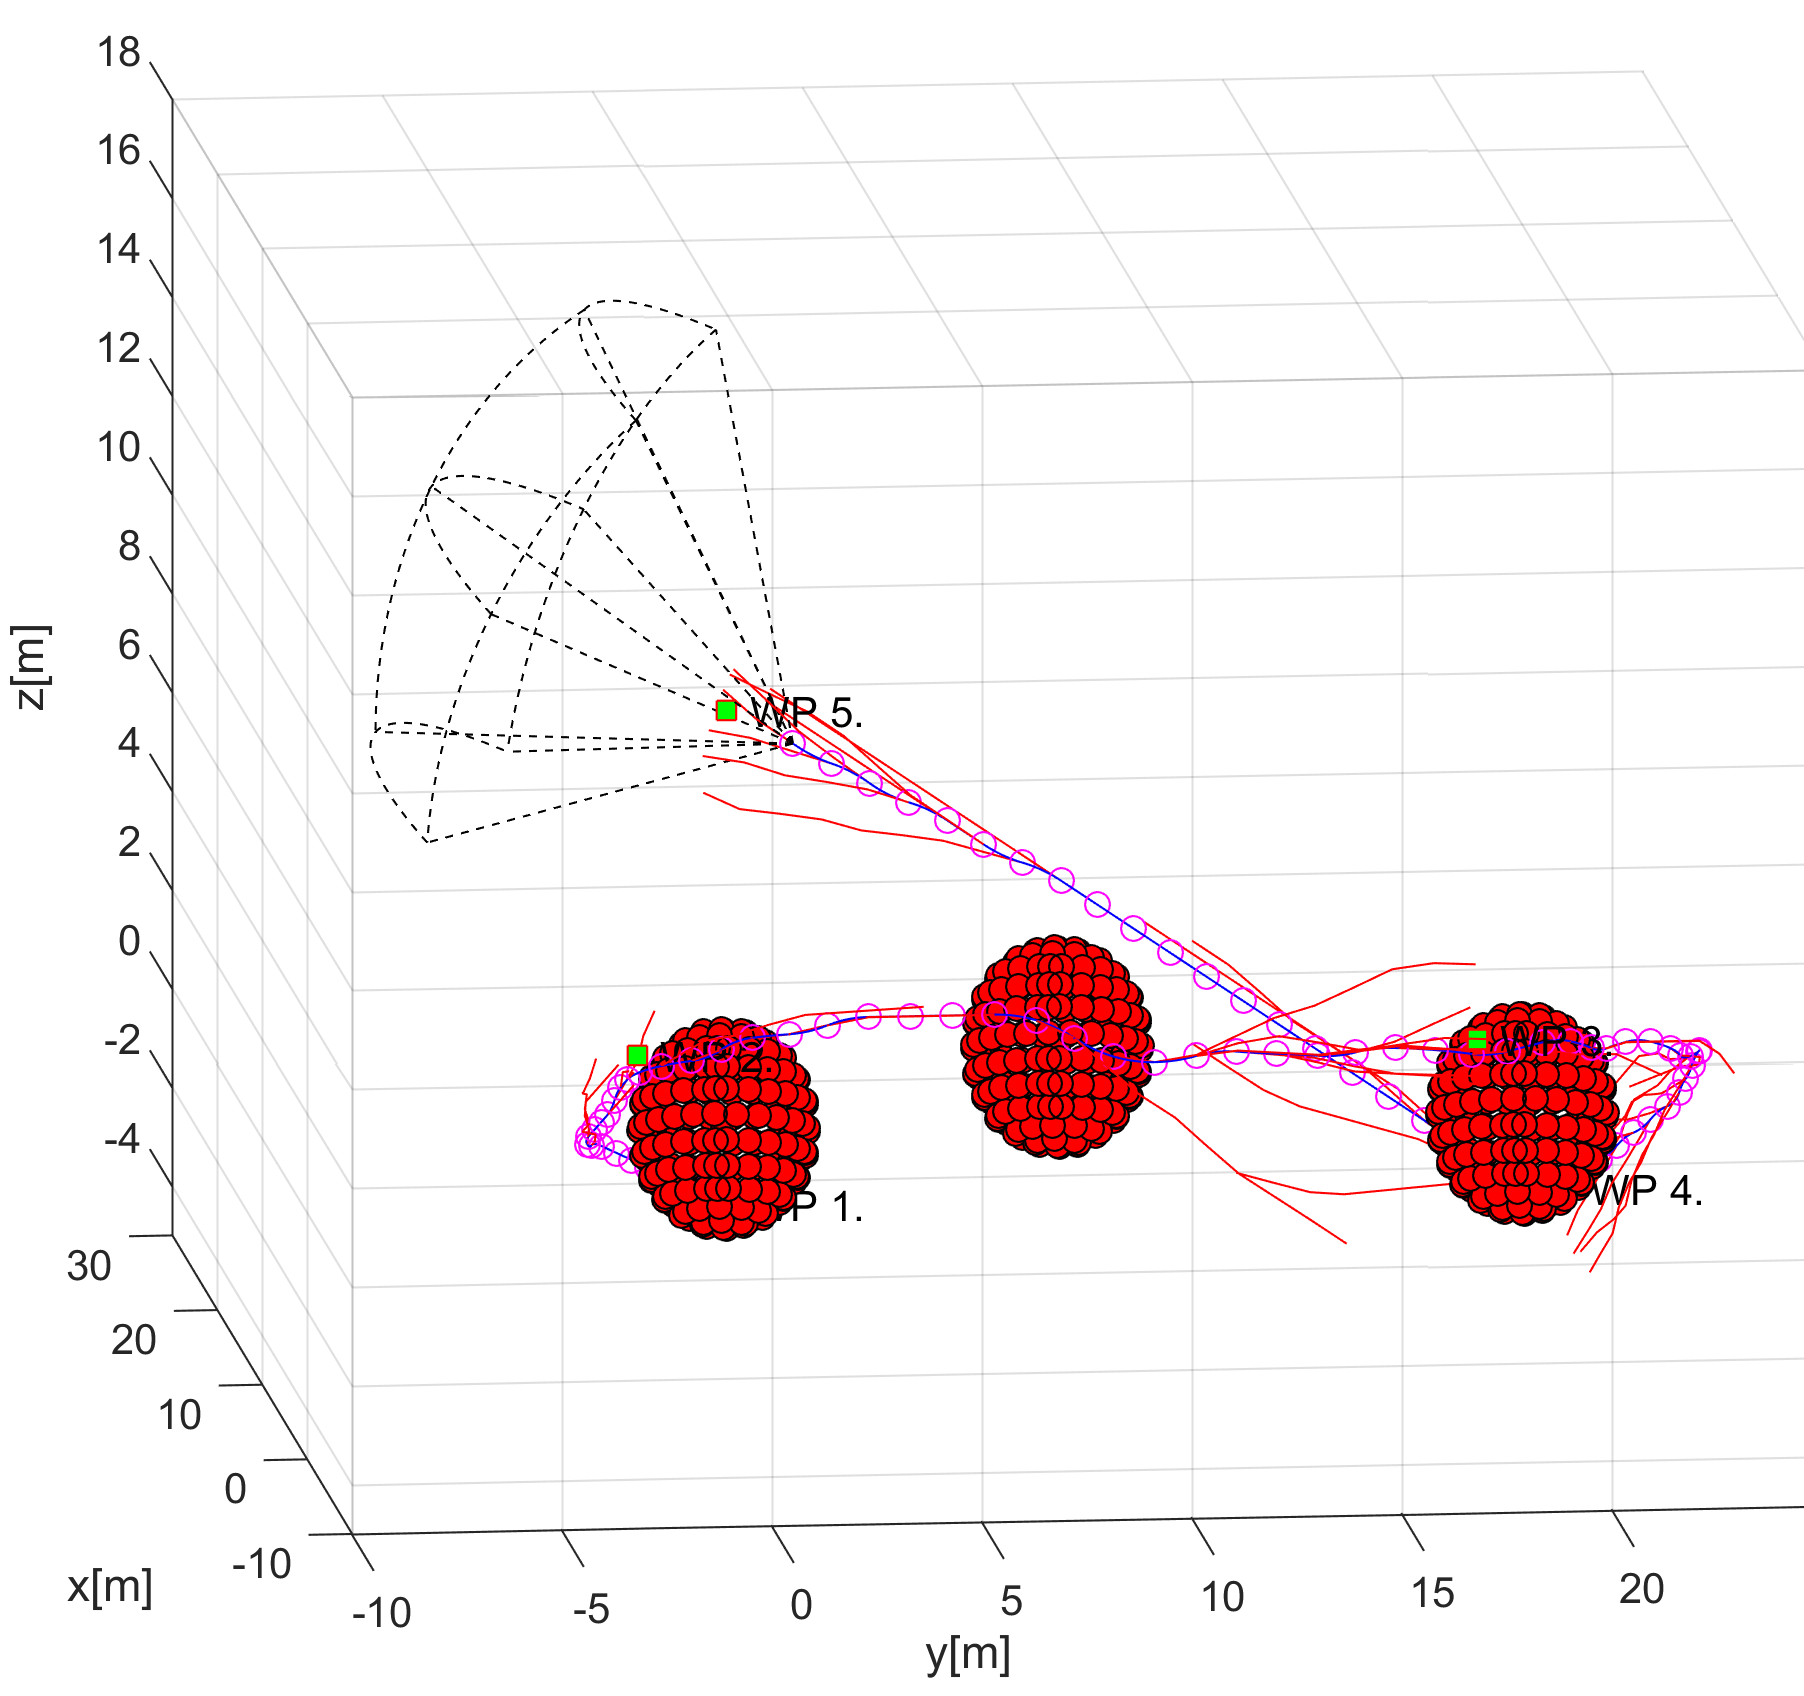
\includegraphics[width=\textwidth]{\FIGDIR/P37FullAvodanceStaticObstacle}
    \caption{Vehicle trajectory after mission competition}
    \label{fig:P37FullAvodanceStaticObstacle}
\end{figure}

\subsection{Probabilistic model evaluation}\label{sec:probabilisticModelEvaluation}
\noindent The \emph{general algorithm} (\ref{eq:mainRatingInputs},\ref{eq:mainRatingCalculation}), defines multiple probabilities for cells $c_{i,j,k}\in\mathscr{A}$ and trajectories $\mathscr{T}\in\mathscr{R}$, in case of static obstacle avoidance the key focus probabilities are following:
\begin{enumerate}
    \item\emph{Reachibility probability} $P_{R}(c_{i,j,k})$, $P_{R}(\mathscr{T}(x_0,B))$ - the the reachability was impacted by obstacle space $\mathscr{O}$ and visibility, for sake of simplicity the reachability was reaching only two values $P_{R}\in \{0,1\}$ .
    \item\emph{Obstacle probability} $P_{O}(c_{i,j,k})$ - obstacle probability in cell was assessed using general algorithm (\ref{eq:mainRatingInputs},\ref{eq:mainRatingCalculation}) and detected obstacle probability $P_{O_D}$ (\ref{eq:detectedObstacleProbability}).
    \item\emph{Visibility probability} $P_{O}(c_{i,j,k})$ - calculated according to standard visibility formula $P_V(c_{i,j,k})$ (\ref{eq:FinalVisibilityProbability}).
\end{enumerate}


\begin{figure}[H]
    \centering
    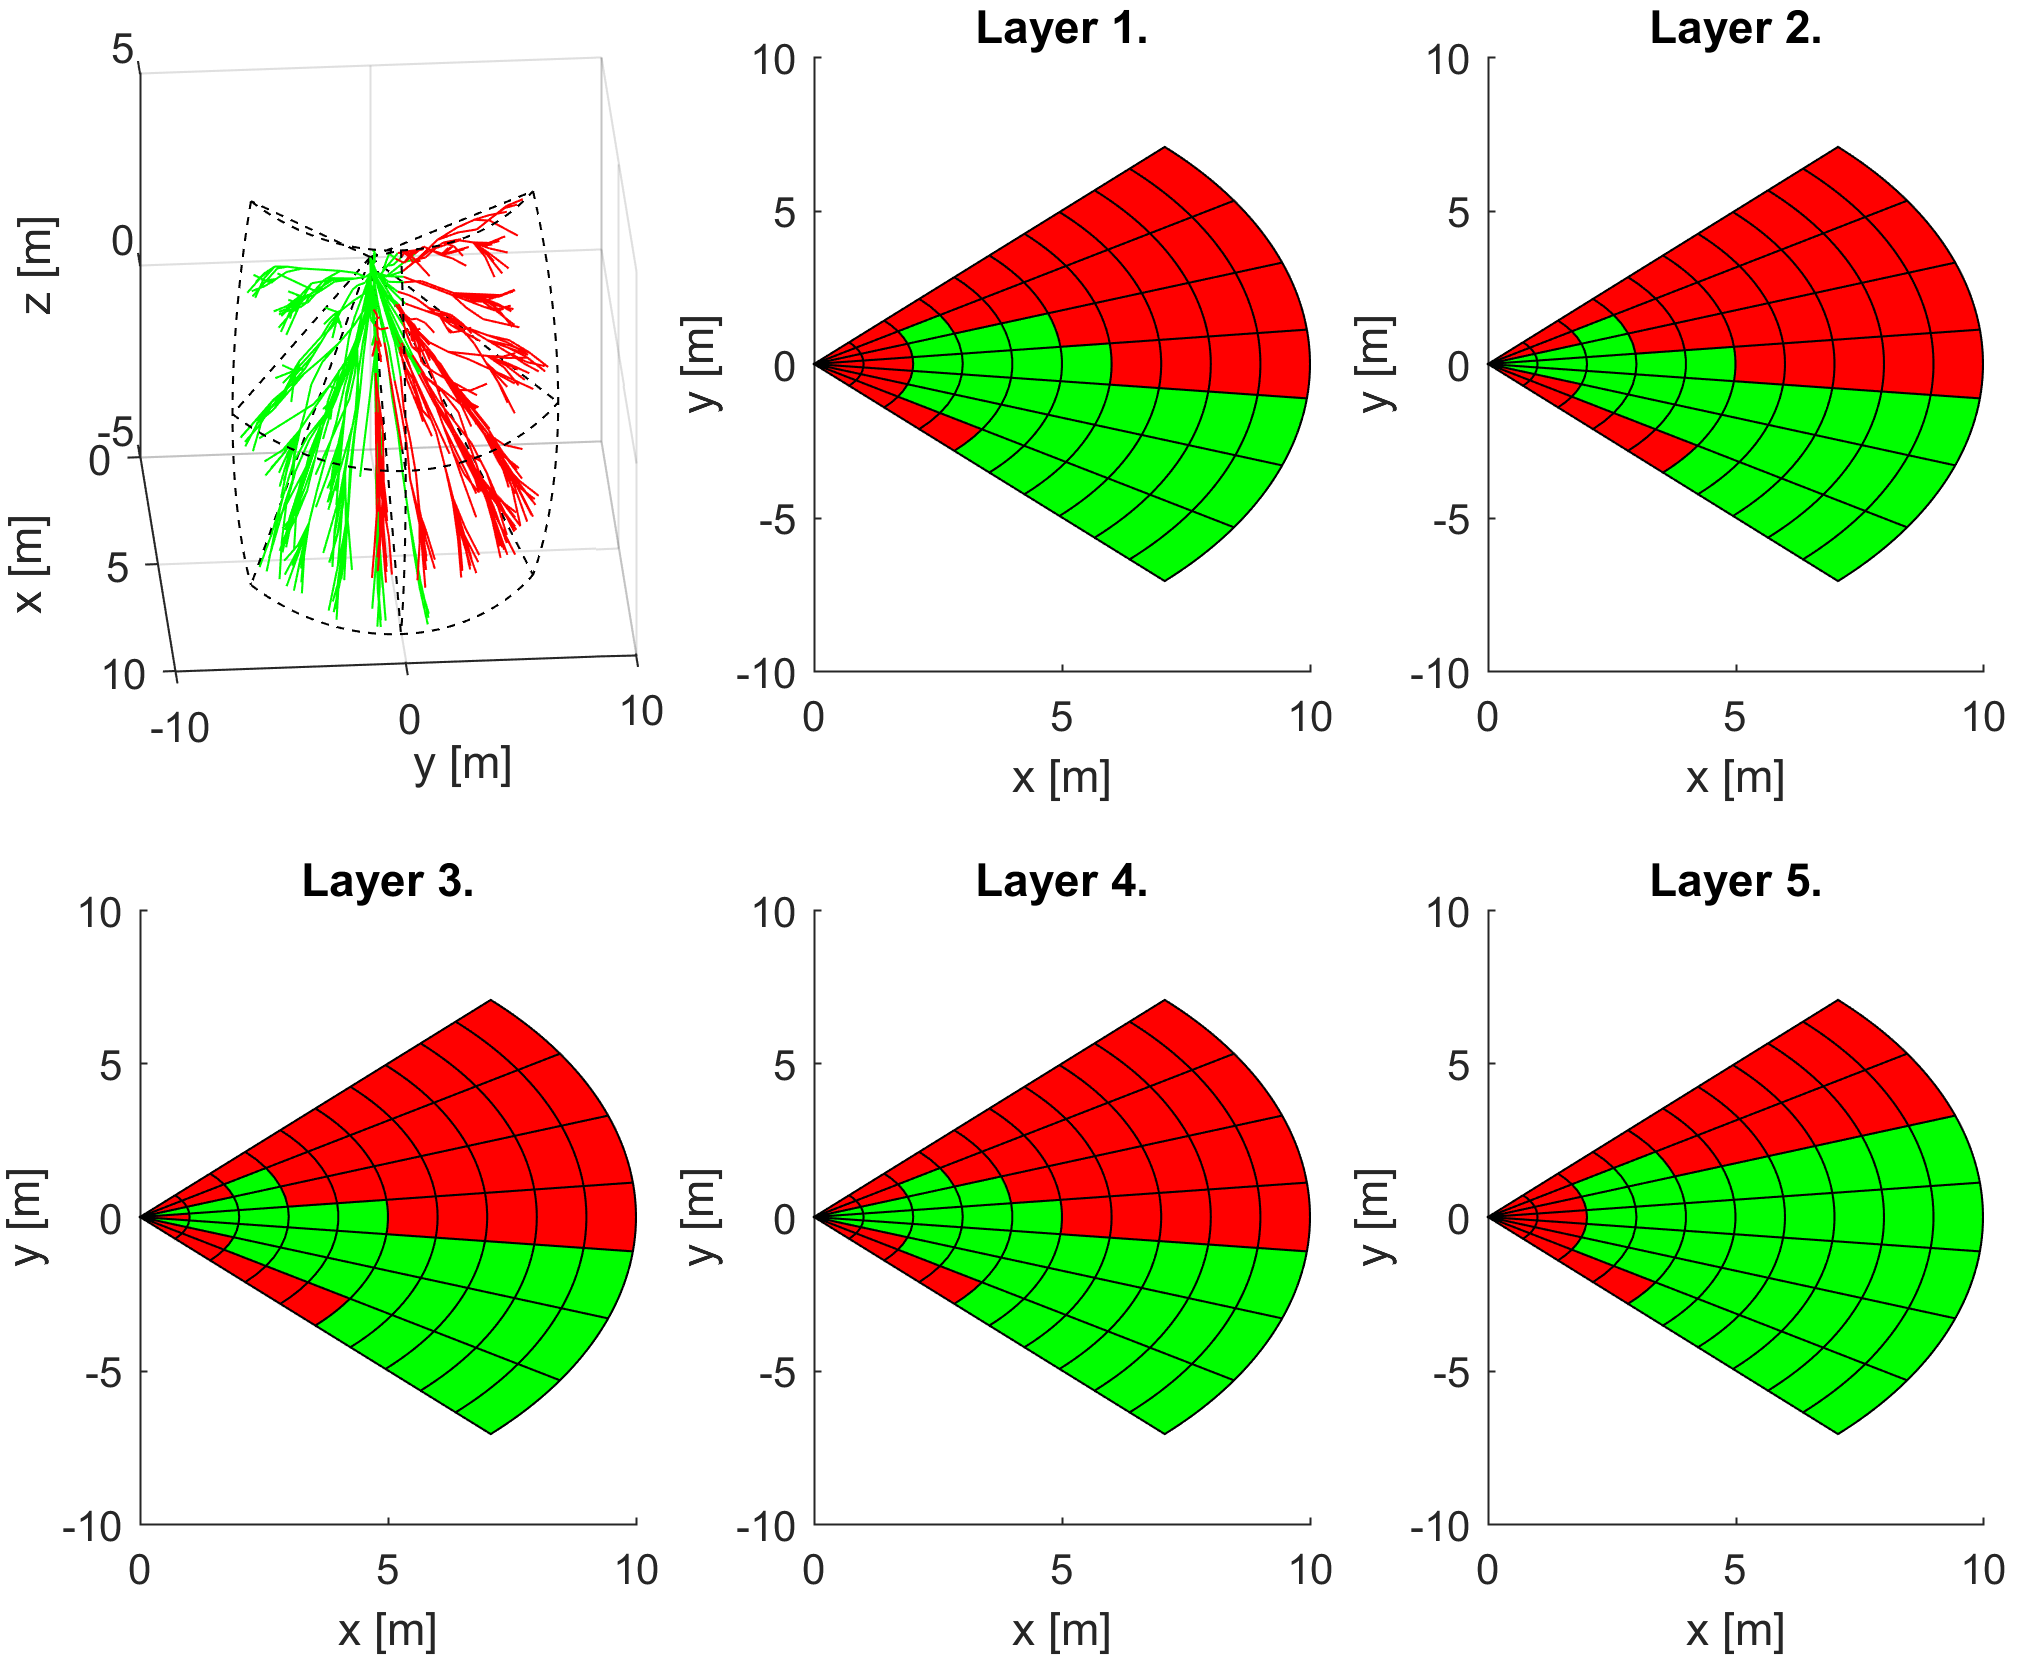
\includegraphics[width=\textwidth]{\FIGDIR/P32ReachableSpaceExampleStatic}
    \caption{Reachability probability assessment for $\mathscr{B}_\mathscr{O}(1)$ avoidance}
    \label{fig:P32ReachableSpaceExampleStatic}
\end{figure}
\noindent For intersection please refer to \emph{first obstacle set $\mathscr{B}_\mathscr{O}(1)$ avoidance} (fig. \ref{fig:P31FirstObstacleAvoidance}). The obstacle space is slightly in right-upper quadrant (from vehicles viewpoint). The red trajectories are leading to obstacle or trough obstacle space, the green trajectories are leading trough or to safe space. \emph{Layer 1.-5.} right part is not reachable (red cells), there is possible escape paths on left side (green cells).

\begin{figure}[H]
    \centering
    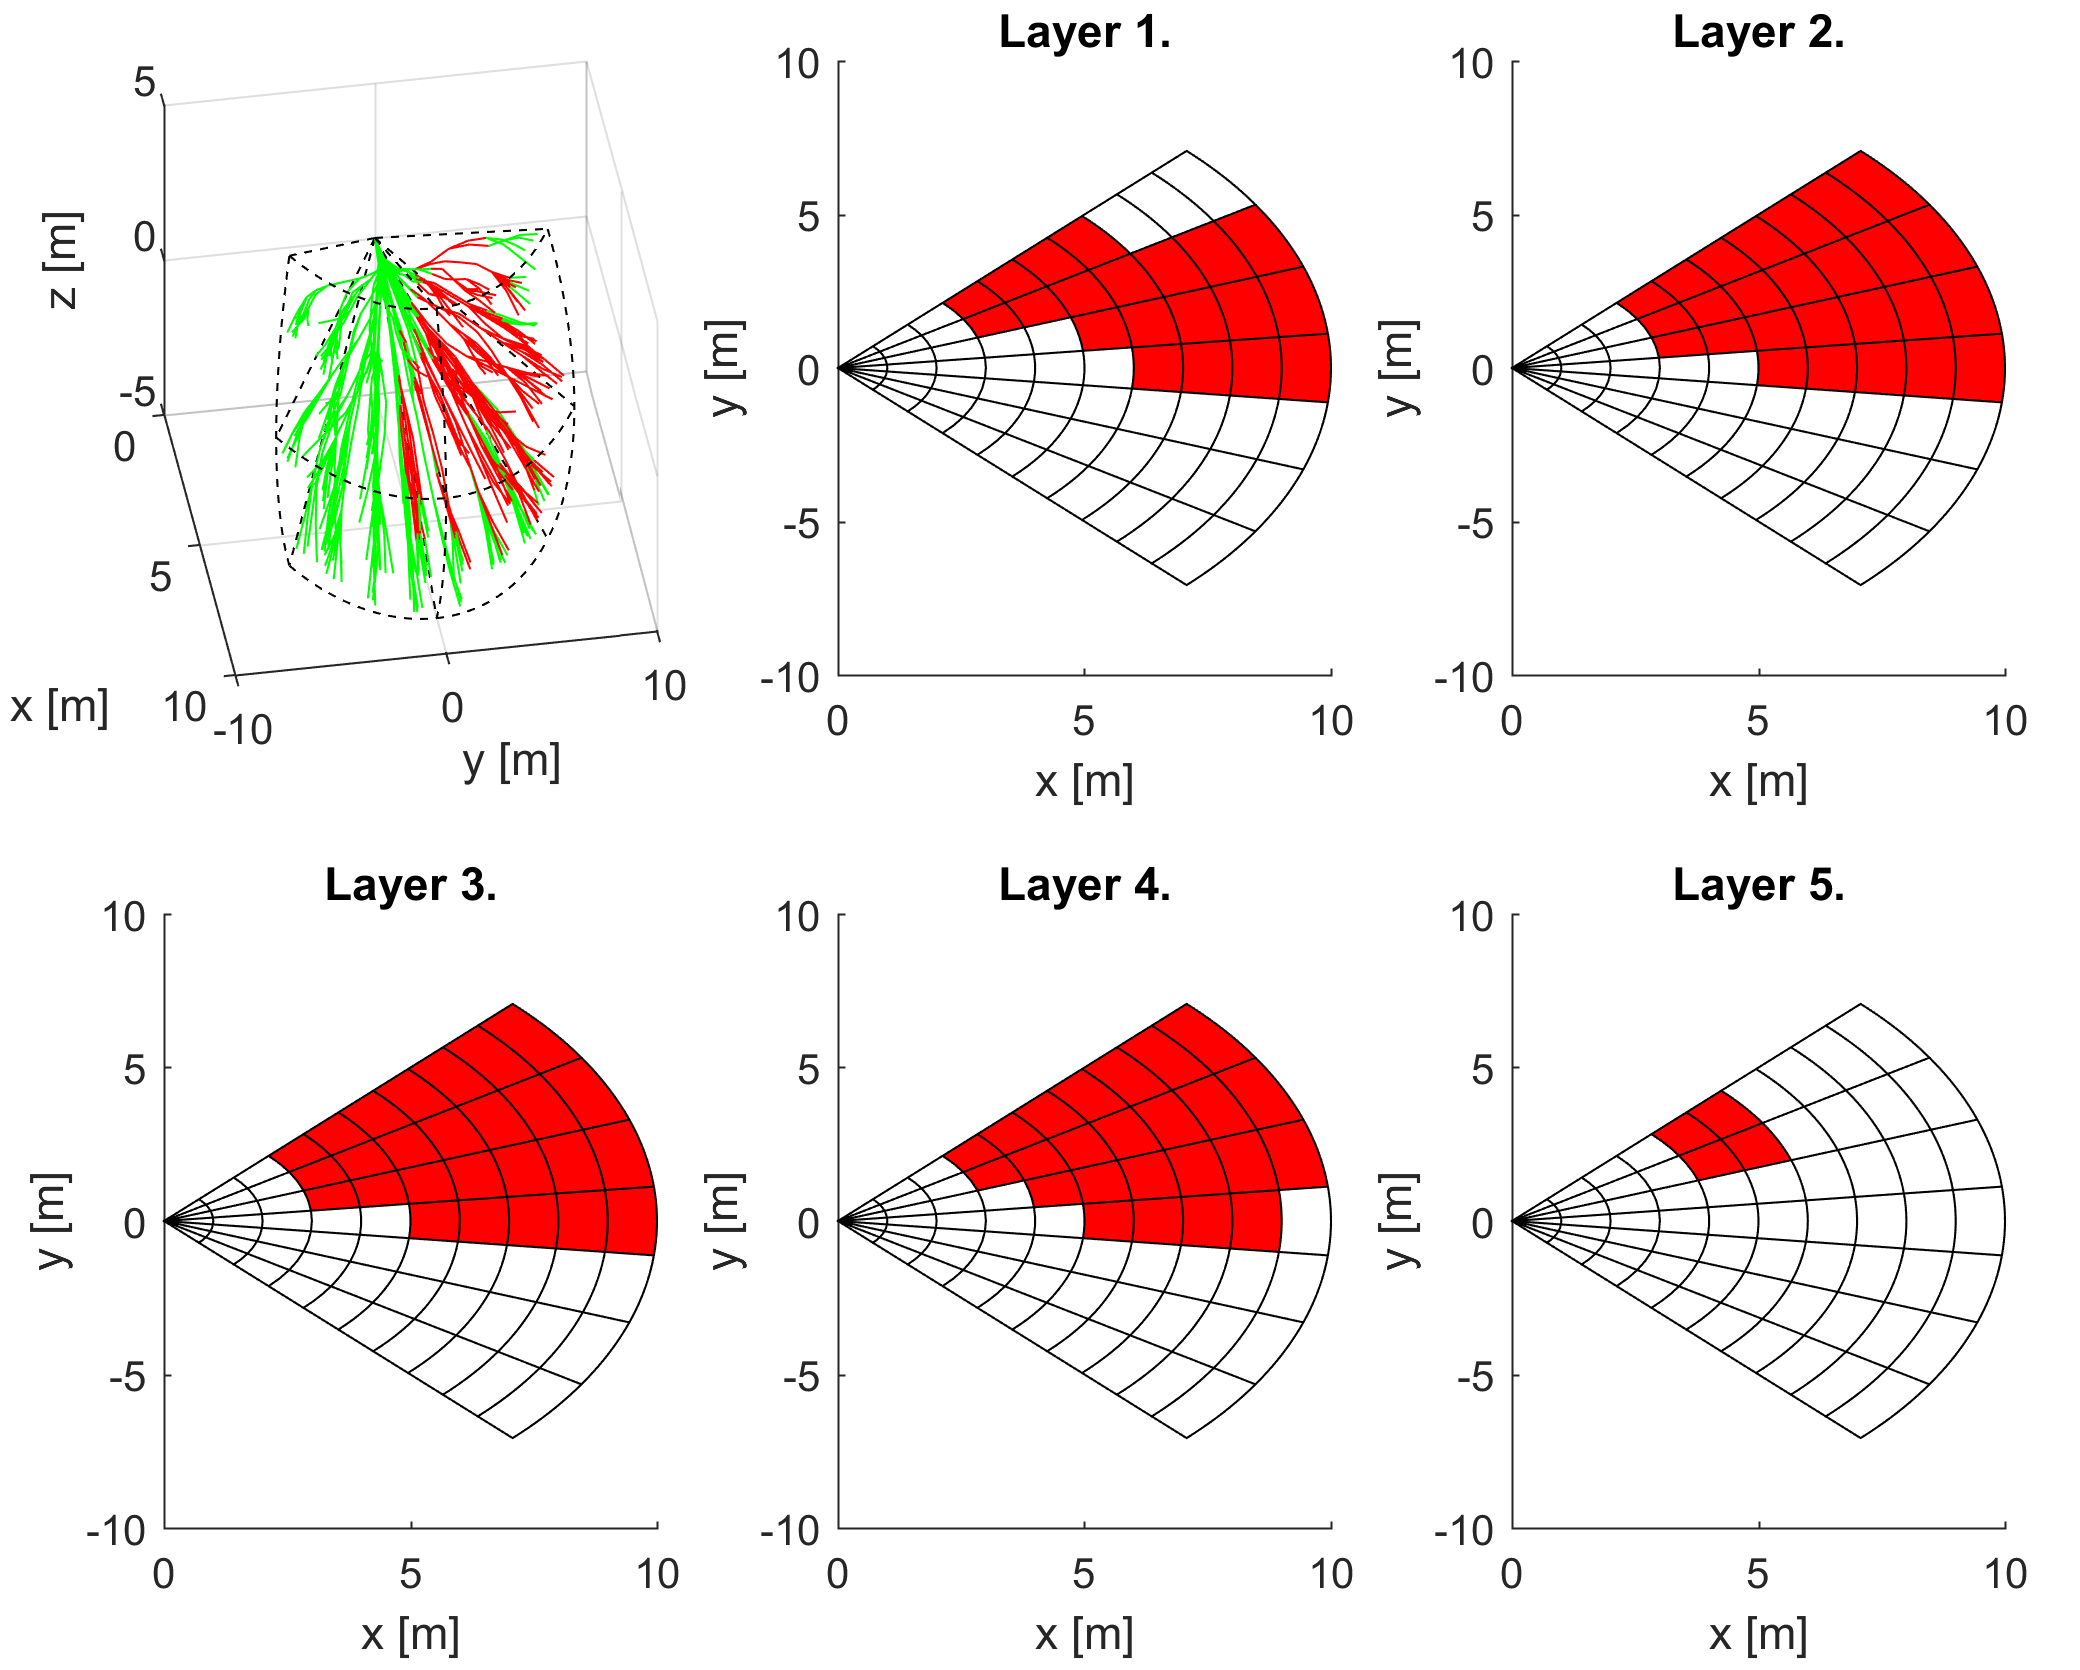
\includegraphics[width=\textwidth]{\FIGDIR/P33ObstacleSpaceStaticExample}
    \caption{Obstacle probability assessment for $\mathscr{B}_\mathscr{O}(1)$ avoidance}
    \label{fig:P33ObstacleSpaceStaticExample}
\end{figure}
\noindent For intersection please refer to \emph{first obstacle set $\mathscr{B}_\mathscr{O}(1)$ avoidance} (fig. \ref{fig:P31FirstObstacleAvoidance})
The obstacle space is slightly in right-upper quadrant (from vehicles viewpoint). The red trajectories are leading to obstacle or trough obstacle space, the green trajectories are leading trough or to safe space. The obstacle space accounts only visible part of the obstacle, therefore in \emph{layer 1. and 4.} is space which is considered without obstacle (white cells). The obstacle space (red cells) in bottom layer (\emph{layer 5.}) is very small due the vehicle is tilted down a little in time of obstacle assessment.

\begin{figure}[H]
    \centering
    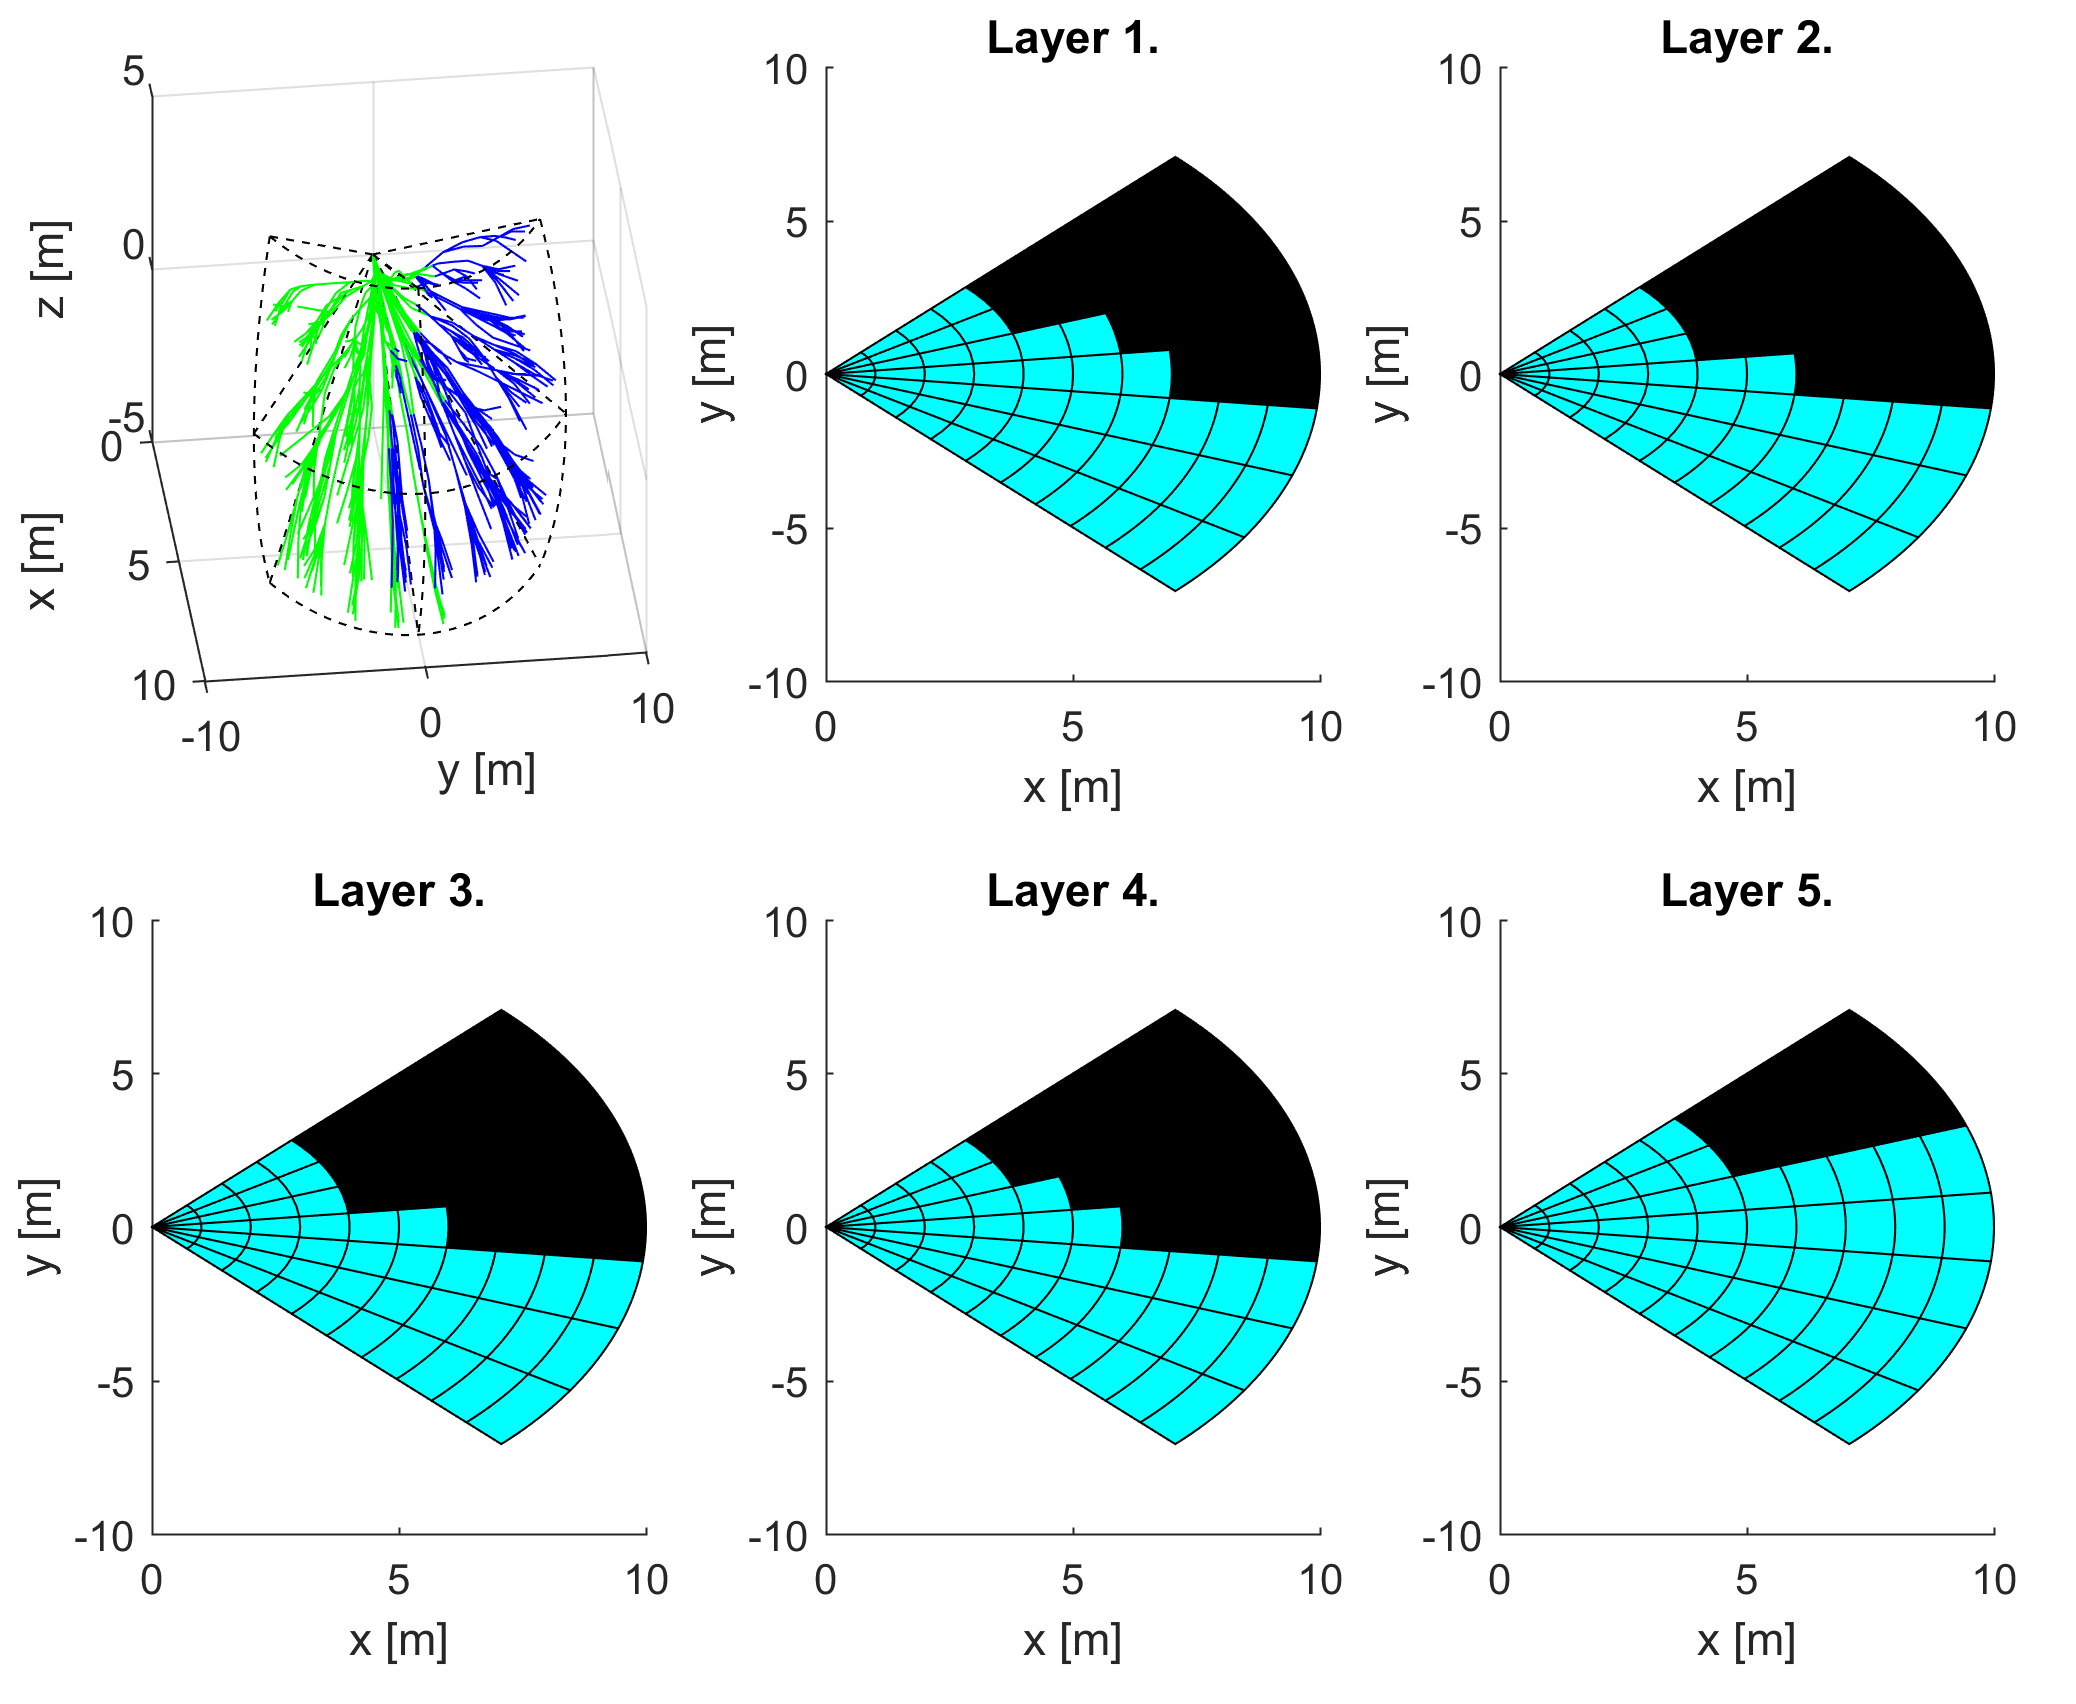
\includegraphics[width=\textwidth]{\FIGDIR/P34VisibleSpaceStaticExample}
    \caption{Visibility probability assessment for $\mathscr{B}_\mathscr{O}(1)$ avoidance}
    \label{fig:P34VisibleSpaceStaticExample}
\end{figure}
\noindent For intersection please refer to \emph{first obstacle set $\mathscr{B}_\mathscr{O}(1)$ avoidance} (fig. \ref{fig:P31FirstObstacleAvoidance}). 
The \emph{visibility space is obscured }


\subsection{Avoidance performance}\label{sec:avoidancePerformacne}
\noindent \emph{Obstacle avoidance performance} for autonomous systems is evaluated by multiple criteria. A necessary condition is \emph{crash distance $d_c$ does not cross safety margin $s_m$}. In the other world that vehicle does not crash into static obstacle. 

\emph{The sufficient conditions} are following:
\begin{enumerate}
    \item\emph{Energy consumption} - For each system $\dot{x}=f(x,u)$ cost functional $J(x,u,t)$ can be proposed to reflect system performance or energy consumption. This functional is therefore used in optimization maximization/minimization problem.
    \item\emph{Trajectory tracking} - Trajectory of vehicle is given by ordered set of waypoints $\mathscr{WP}=\{W_1,W_2,\dots,W_i\}$. The given trajectory may not be feasible for vehicle system $\dot{x}=f(x,u)$. To differentiate the performance of tracking Mean Square error is introduced like following:
    \begin{equation}
        e= \sqrt{\left((\hat{x}(t)\to\R^k)-(x(t)\to\R^k)\right)^2}
    \end{equation}
    \noindent Where $(\hat{x}(t)\to\R^k)$ is expected parameters projected to space $\R^k$ and $(x(t)\to\R^k)$ is real system performance projected to same space. Usually performance parameter is deffined as deviation from projected trajectory $\tilde{x}(t)\in\R^3$.
\end{enumerate}

\begin{figure}[H]
    \centering
    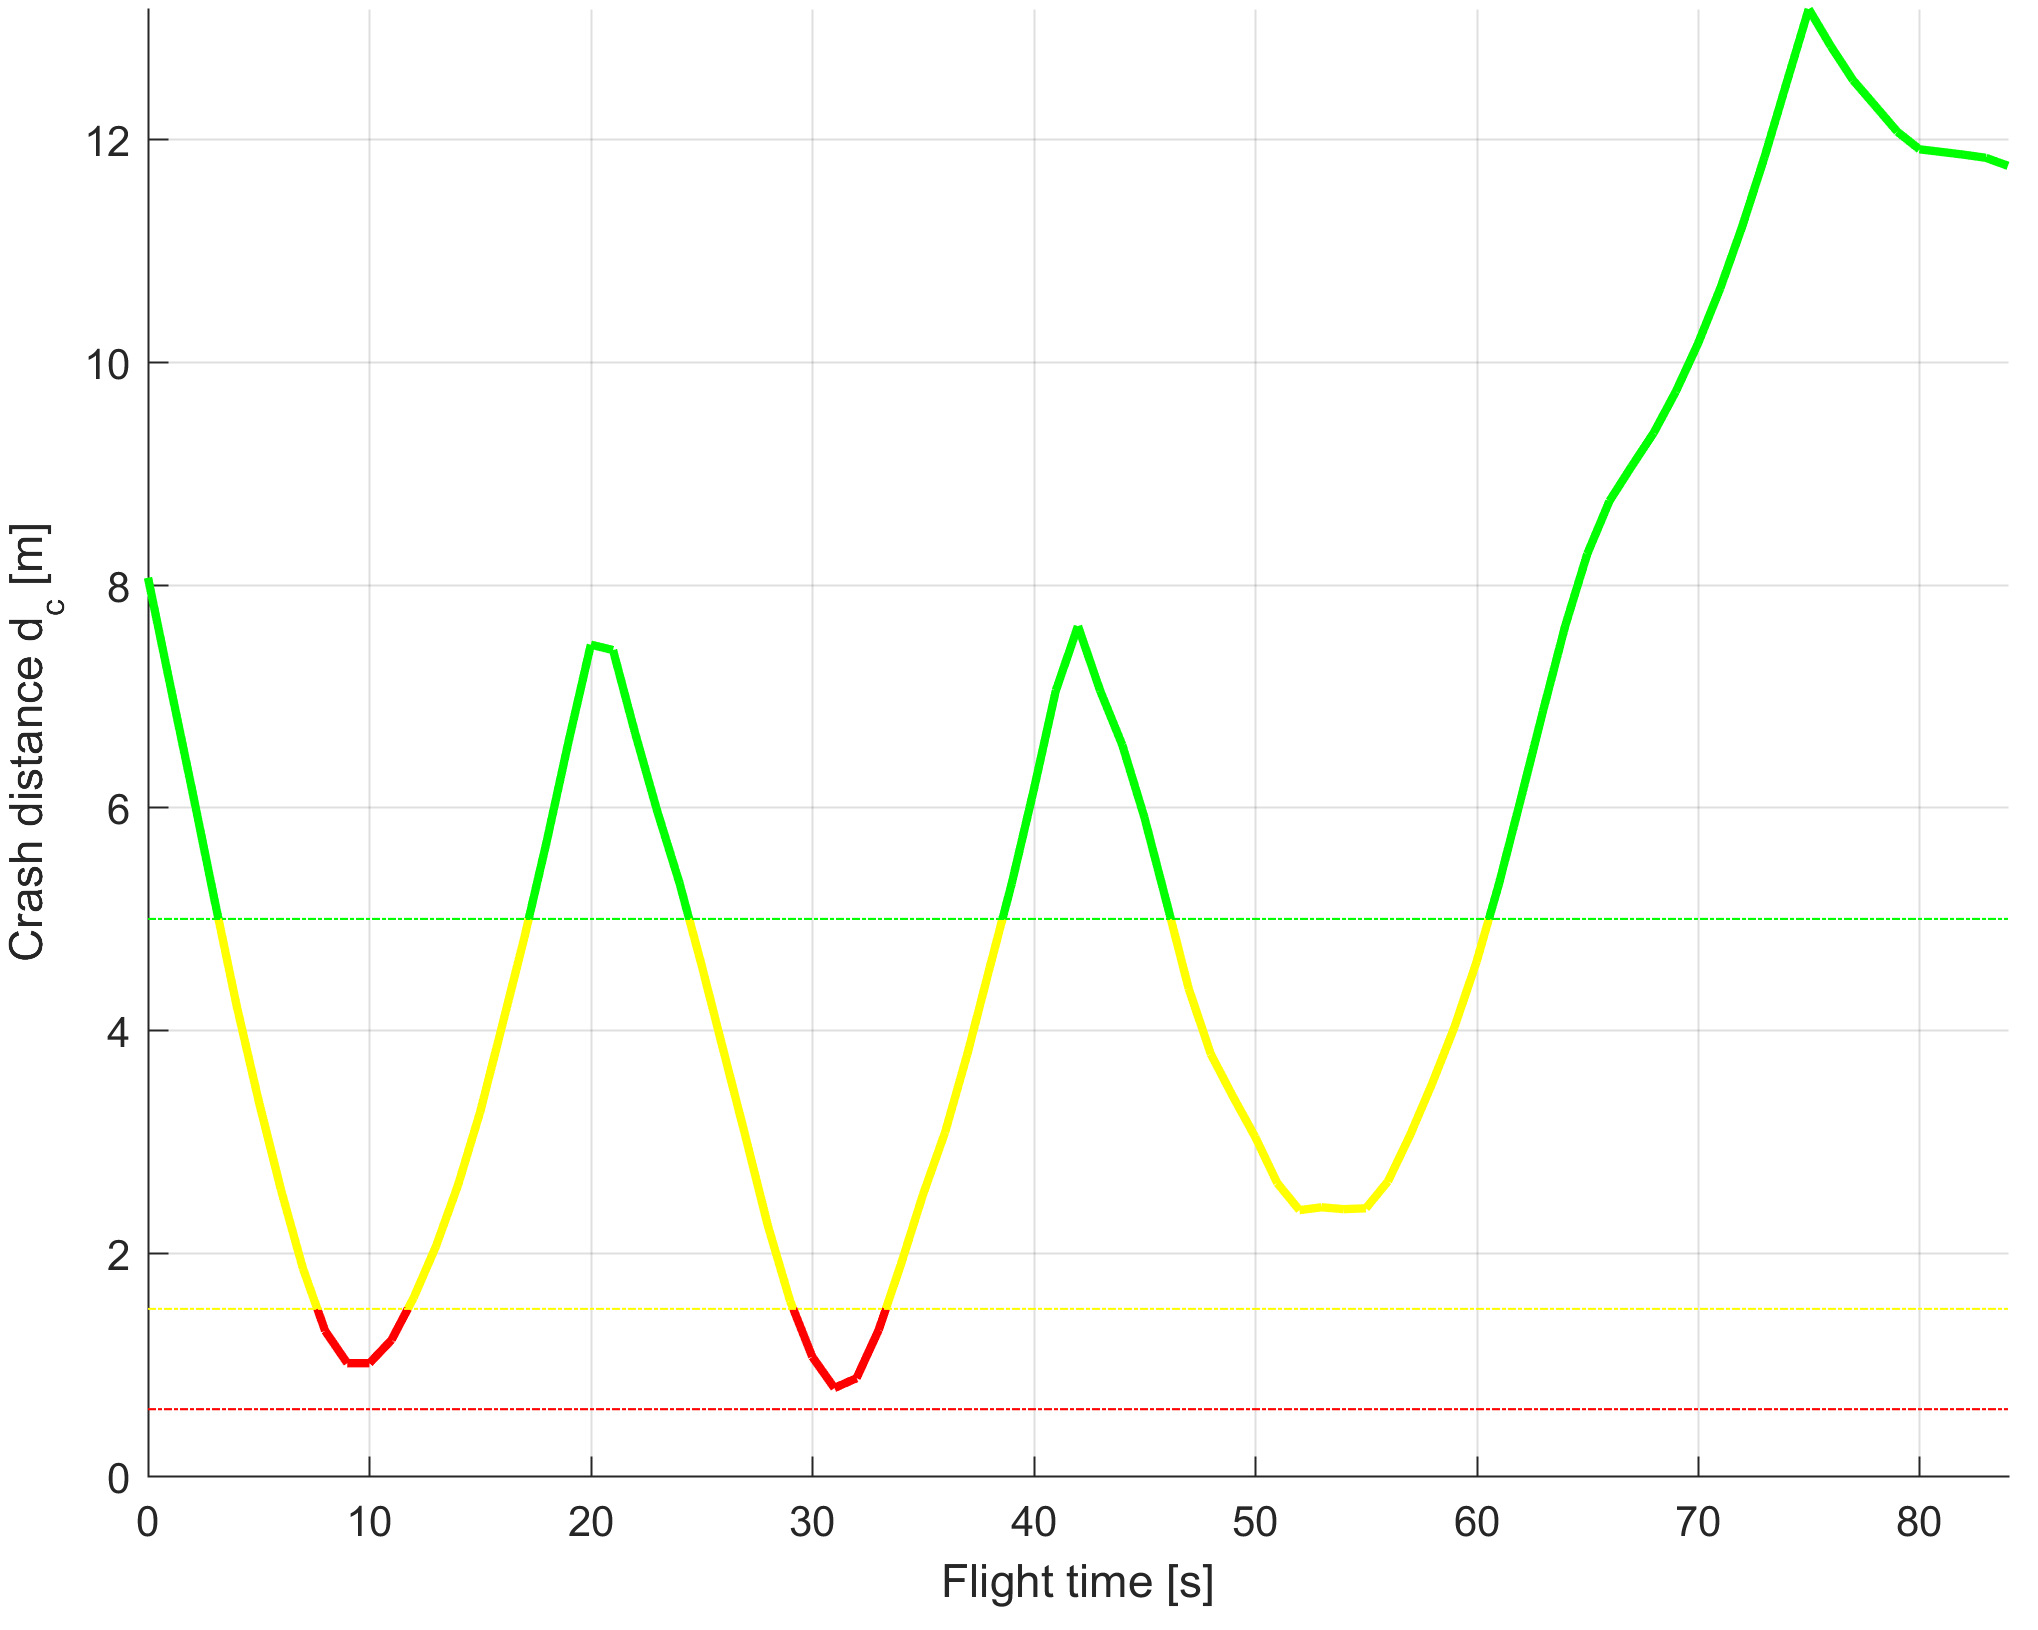
\includegraphics[width=\textwidth]{\FIGDIR/P38CrashDistanceEvolutionWide}
    \caption{Crash distance $c_r$ evolution during mission}
    \label{fig:P38CrashDistanceEvolutionWide}
\end{figure}

\noindent \emph{Crash distance to nearest obstacle evolution} (fig \ref{fig:P38CrashDistanceEvolutionWide}) displays how far vehicle was to nearest obstacle during the mission execution. There are three lines representing:
\begin{enumerate}
    \item\emph{Conservative methods margin $c_m$} (green dashed line) - conservative methods are based on simple preposition \emph{turn back while you can}, therefore conservatives methods margin $c_m$ is calculated like follow:
    \begin{equation}
        c_m = 
        \begin{aligned}
            &2\times r_t + 3 \times r_v\\
            &2 \times 2m + 3\times 0.6m\\
            &4.6m
        \end{aligned}
    \end{equation}
    \noindent Where $r_t$ is turning radius of vehicle and $r_v$ is radius of vehicle. The conservative methods margin $c_m$ is $4.6$ meters for given simulation parameter. 
    
    \item\emph{Adaptive methods margin $a_m$} (yellow dashed line) - are more energy consumption focused. The focus is on not deviating from optimal trajectory as long as possible. Typical representative of adaptive algorithms is potential field avoidance algorithm. The \emph{potential field avoidance} principle is following: Each  obstacle (static or moving) has a potential like a magnet, our vehicle has inverse potential. The magnitude of potentials can change over time depending on various factors (like the danger level etc.). The margin of adaptive methods was calculated by following formula:
    \begin{equation}
        a_m = 6 \times r_v = 6 times 0.3 = 1.8 m
    \end{equation}
    \noindent Where $r_v$ stands for vehicle radius. The adaptive methods margin $a_m$, where the \emph{potential field method} is key comparison element is $1.8$ m
    
    \item\emph{Safety margin $s_m$} (red dashed line) has been discussed in section \ref{sec:staticObstacleAvoidanceSimulation}. Safety margin of our method $s_m$ is set as $60 cm$
\end{enumerate}

\noindent\emph{The crash distance $c_r{t}$} never breaches $d_c(t) \ge s_m$ therefore \emph{necessary condition} is satisfied. The \emph{proposed approach} outperforms \emph{conservative methods} $\exists t, d_c (t) \le c_m$ (yellow part of $d_c$ evolution) also outperforms \emph{adaptive methods}, because $\exists t, d_c(t)\le a_m$.

\begin{figure}[H]
    \centering
    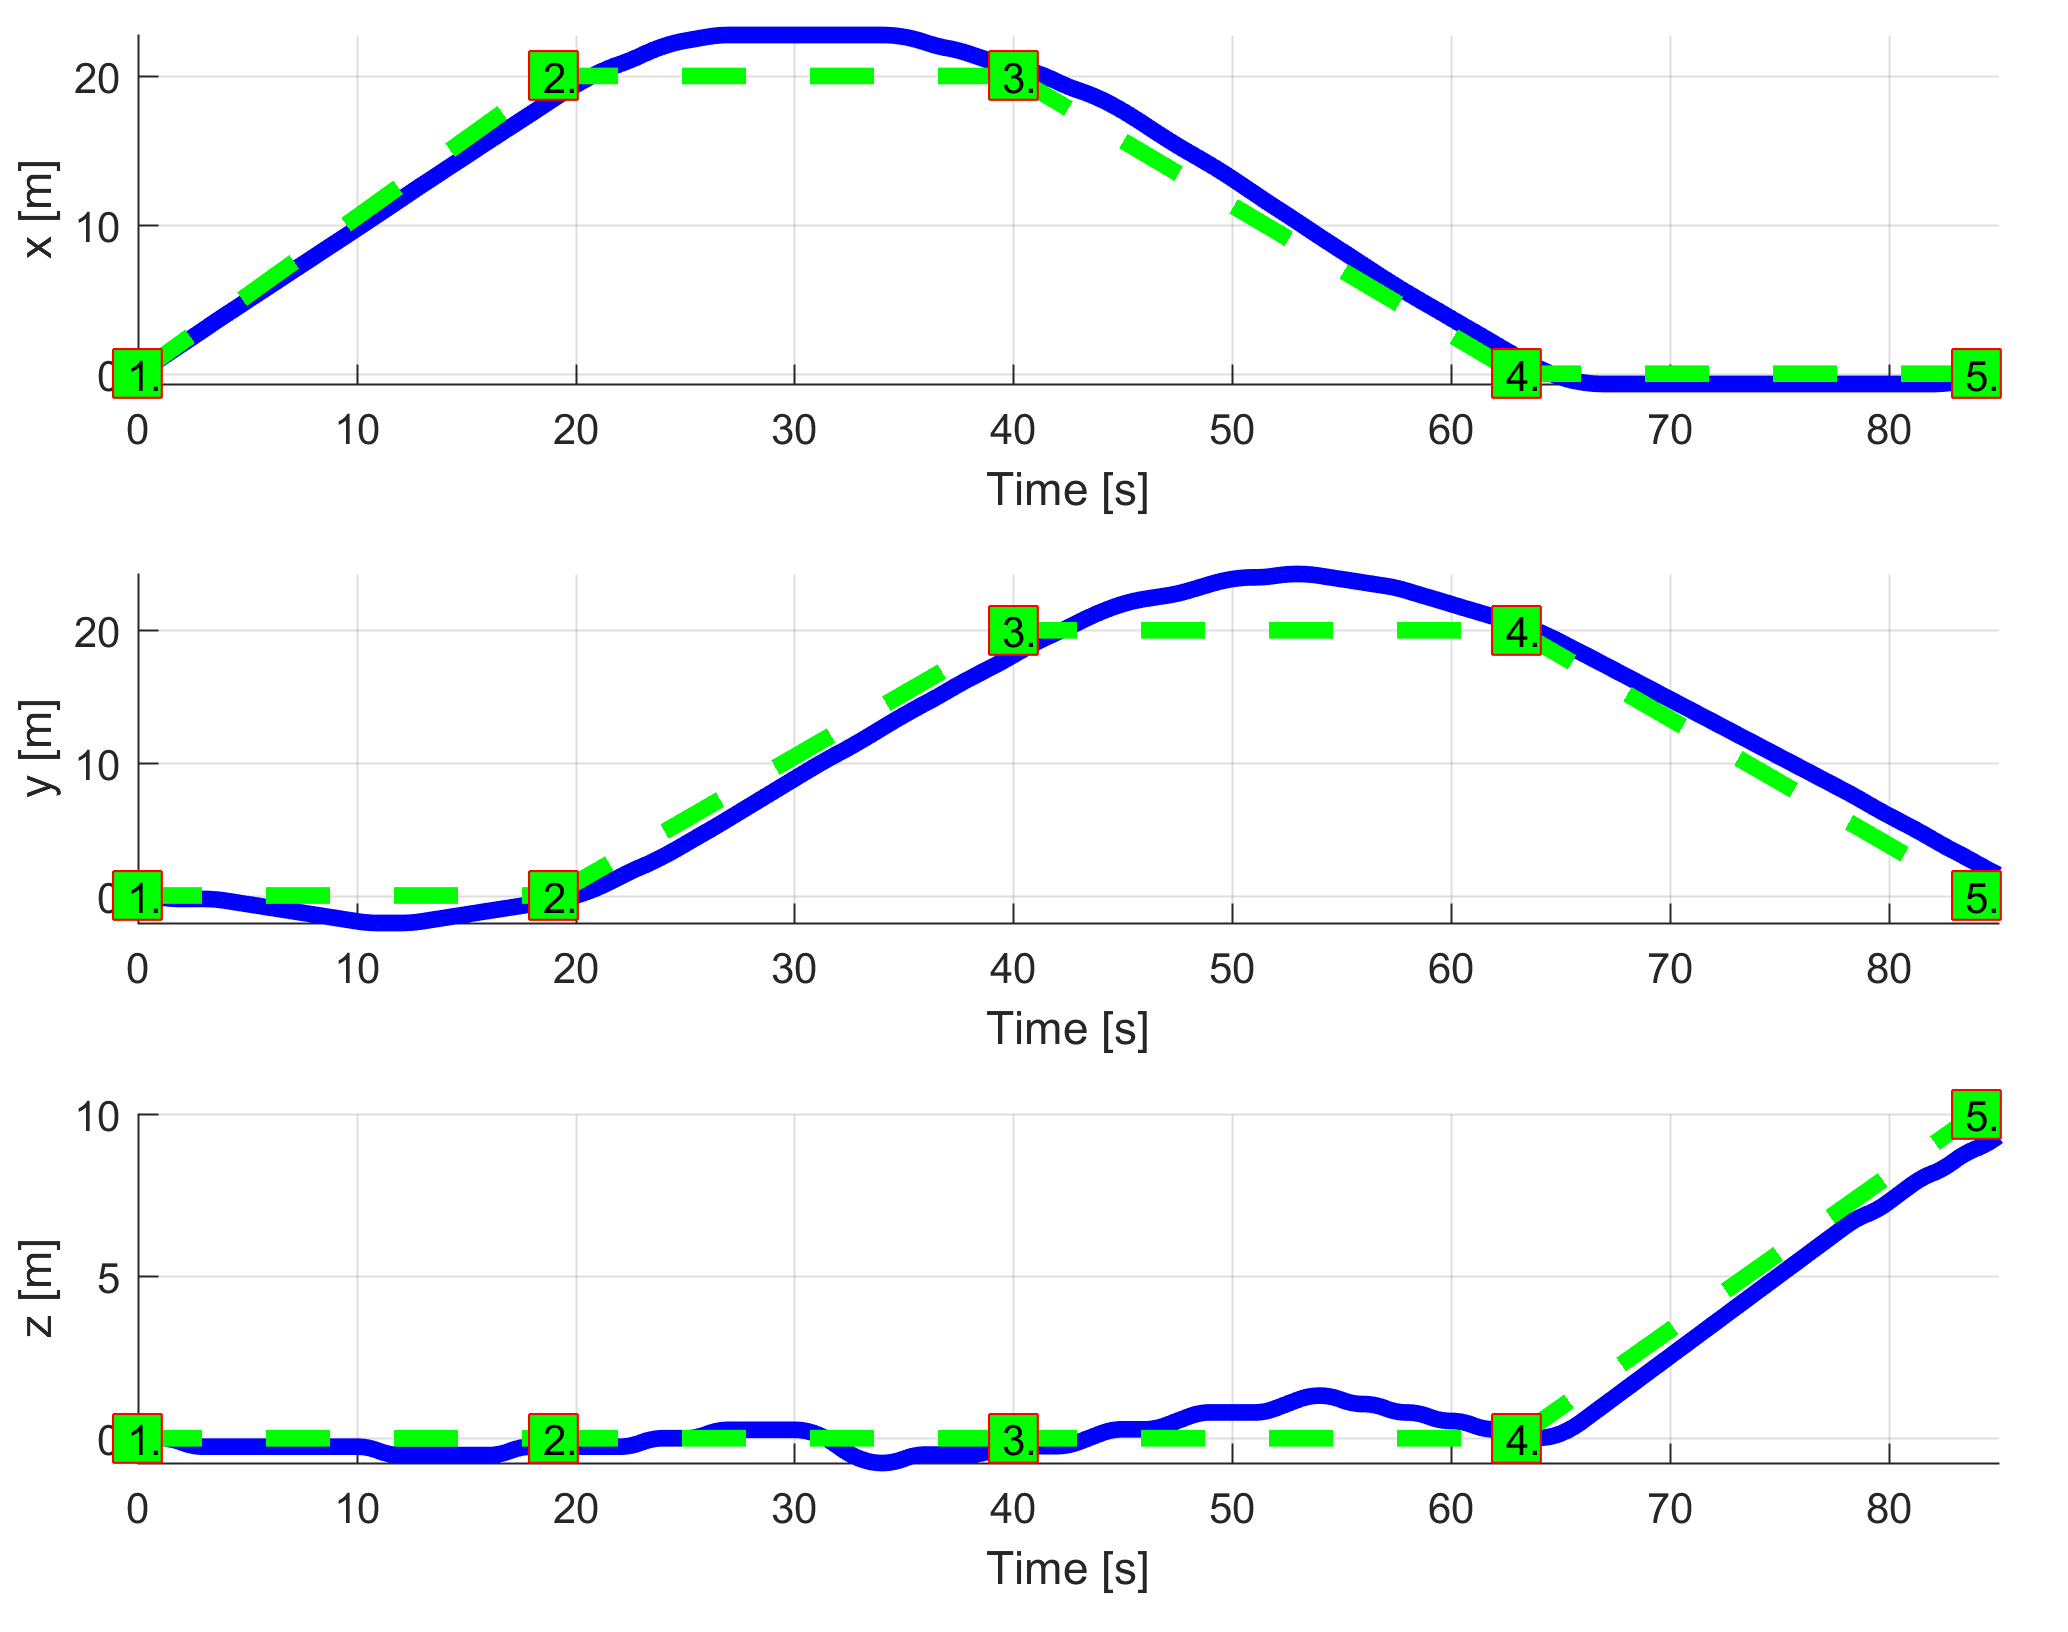
\includegraphics[width=\textwidth]{\FIGDIR/P39TrajectoryTrackingPerformance}
    \caption{Trajectory tracking performance}
    \label{fig:P39TrajectoryTrackingPerformance}
\end{figure}

\noindent\emph{Trajectory tracking performance} (fig. \ref{fig:P39TrajectoryTrackingPerformance}) displays trajectory tracking problem divided into state tracking problem of $x(t)$, $y(t)$, and $z(t)$. The ordered waypoint set $\mathscr{WP}$ is displayed as numbered green squares. The \emph{desired trajectory} $\hat{x}(t)$, $\hat{y}(t)$, and $\hat{z}(t)$ is displayed as green dashed line between waypoints. The \emph{vehicle performance} $x(t)$, $y(t)$, and $z(t)$ is displayed as blue  line. 

\emph{Overall performance} is optimal in avoidance grid $\mathscr{A}(t_i)$ and semi-optimal in joined trajectory $\mathscr{T}(x_0,B_1,\dots,B_i)$ \cite{alojzgomola2017}. This property transits from deterministic approach and its kept based on given threshold.

\section{Intruders avoidance}
\noindent \emph{Intruder avoidance} have been studied on set of avoidable intruders which maneuverability and velocity was smaller or equal to vehicle  velocity and maneuverability.
\noindent The ordered waypoint set $\mathscr{WP}$ is defined as follow:
\begin{enumerate}
    \item\emph{Starting waypoint $W_1$} - $[0,0,0]$ - not necessary, just to emphasize the local coordinate frame center
    \item\emph{Final waypoint $W_2$} - $[55,0,0]$.
\end{enumerate}


\noindent Other simulation parameters are stated like follows:
\begin{enumerate}
    \item\emph{Vehicle model $\dot{x}=f(x,u)$} is given by eq. \ref{eq:simple3ddifferentialequations}.
    \item\emph{Vehicle control $\mathscr{MA}$} is defined in section \ref{ch:movementAutomatonPredictor}.
    \item\emph{Vehicle body radius $r_b$} is given as 30 cm.
    \item\emph{Intruder horizontal spread} is estimated as $\pi/16$ [rad] for each intruder $i_k\in\mathscr{I}$.
    \item\emph{Intruder vertical spread} is estimated as $\pi/24$ [rad] for each intruder $i_k\in\mathscr{I}$.
    \item\emph{Vehicle turning radius $r_t$} is given as 2 m, this parameter impacts the decision time $t_i$ selection based on the in-veritable crash distance \cite{alojzgomola2017}.
    \item\emph{Movement automaton prediction error $E_p=(\mathscr{MA}$)} is equal to 30 cm.
    \item\emph{Safety margin $s_m$} is set to 60 cm.
    \item\emph{Avoidance grid $A(t_i) $}properties were set as follow:
    \begin{enumerate}[a.]
        \item start distance $d_s$ 0 m,
        \item end distance $d_e$ 10 m,
        \item step distance $s_d$ 1 m (10 layers),
        \item horizontal span from $\theta_s$ as $-\pi/4$ to $\theta_e$ to $\pi/4$,
        \item horizontal cell count $c_h$ as $7$,
        \item vertical span from $\varphi_s$ as $-\pi/6$ to $\varphi_e$ to $\pi/6$,
        \item vertical cell count $c_v$ as $5$ (layer count).
    \end{enumerate}
    \item\emph{Intruders set} $\mathscr{I}$ is expanding over mission time $t\in[t_s,t_e]$ and each intruder $i\in\mathscr{I}$ is detected at least at border of FOV.
\end{enumerate}

\noindent\emph{Intruder set} $\mathscr{I}$ (tab \ref{tab:intruderSet}) contains set of eight intruders $i_1,\dots,i_8$ which are discovered at mission times $t=5,\dots,40$ seconds. The intruder initial position $\vec{x}_{l}(t_D)$ is in 3D local coordinate frame given by vehicle $\vec{x}(t)$ (\ref{eq:simple3ddifferentialequations}) position and orientation at time of detection $t_D$. The same goes for intruder velocity vector $\vec{v}_{l}(t_D)$. The intruder model (\ref{eq:vehiclelinearcone}) is simple linear line model. 

The intruder intersection model $P_{O_I}(i_k,c_{i,j,k},l,b,s,\tau)$ (\ref{eq:partialProbabilitiesIntruderSummary},\ref{eq:intruderInCellProbabilityOneIntruder}) has following intersection settings:
\begin{enumerate}
    \item\emph{Linear intersection mode} $l$ set as \emph{true}.
    \item\emph{Body volume intersection mode} $b$ set as \emph{false}.
    \item\emph{Ellipsoid cone intersection mode} $s$ set as \emph{true}.
    \item\emph{Timed intersection mode} $\tau$ \emph{false}.
\end{enumerate}

\noindent\emph{Note:} All intruders are attacking vehicle from \emph{left flank} and are discovered at the margin of the FOV. All intruders have speed equal to vehicle speed $v_v$ and its 1 $ms^{-1}$.


\begin{table}[H]
    \centering
    \begin{tabular}{|c||c|c|c|}
        \hline
         Intruder & $t_D$    & $\vec{x}_{l}(t_D)$  & $\vec{v}_{l}(t_D)$ \\\hline\hline
         $i_1$    & $5$ $s$  & $[6,8,-0.5]^T$    & $[0,-1,0]^T$ \\\hline
         $i_2$    & $10$ $s$ & $[6,8,-0.5]^T$    & $[0,-1,0]^T$ \\\hline
         $i_3$    & $15$ $s$ & $[6,8,-0.5]^T$    & $[0,-1,0]^T$ \\\hline
         $i_4$    & $20$ $s$ & $[6,8,-0.5]^T$    & $[0,-1,0]^T$ \\\hline
         $i_5$    & $25$ $s$ & $[6,8,0.5]^T$     & $[0,-1,0]^T$ \\\hline
         $i_6$    & $30$ $s$ & $[6,8,0.5]^T$     & $[0,-1,0]^T$ \\\hline
         $i_7$    & $35$ $s$ & $[6,8,0.5]^T$     & $[0,-1,0]^T$ \\\hline
         $i_8$    & $40$ $s$ & $[6,8,0.5]^T$     & $[0,-1,0]^T$ \\\hline
    \end{tabular}
    \caption{Intruder set $\mathscr{I}$.}
    \label{tab:intruderSet}
\end{table}

\noindent The avoidance of intruders $i_1,i_2,\dots,i_8\in\mathscr{I}$ (tab. \ref{tab:intruderSet}). is shown in figures \ref{fig:P40FirstIntruderSideHit} and \ref{fig:P44IntruderAfterAvoidance}. where:
\begin{enumerate}
    \item\emph{Executed trajectory} (blue line) is trajectory where our vehicle flew in final, this trajectory is keeping safety property ($s_m \ge 1.2m$).
    \item\emph{Planned trajectory} (red line) - at some decision time $t_i$ in avoidance grid $\mathscr{A}(t_i)$ The most feasible trajectory to safely escape is chosen. Because of changing situation, popping up of new intruders in this case, the escape trajectory is often changed (red lines fig. \ref{fig:P41IntruderReachiSet}).
    \item\emph{Avoidance grid} (black dashed line boundary) - avoidance grid is boundary is given by vehicle position and orientation $x(t)\to \R^6$. Its depending on expected vehicle state $\hat{x}(t_i)$ at time of avoidance $t_i$.The boundary of avoidance grid $\mathscr{A(t_i=5s)}$ is in fig. \ref{fig:P39TrajectoryTrackingPerformance}. Plotting avoidance grid $\mathscr{A}$ for each time of decision $t_i$ is pointless, because it will overshadow more important information like, intruder position and planned trajectory.
    \item\emph{Decision point} (empty magenta circle) - shows when vehicle generated new avoidance grid $\mathscr{A}$ for expected state of vehicle $\hat{x}(t)$.
    \item\emph{Waypoints} (numbered green square) - direct line between two waypoint is the shortest distance to fly, the waypoints must be reached in the order.
    \item\emph{Intruder position} (full red circle) - intruder $i_k$ position at decision time $t_i$, this is intruder $i_k$ expected position. 
    \item\emph{Intruder trajectory} (linked full magenta circles) - intruder positions joined via line in previous decision times $t_{i-1},\dots,t_{i-d}$, where $t_{i-d}$ is detection time. 
\end{enumerate}
\begin{figure}[H]
    \centering
    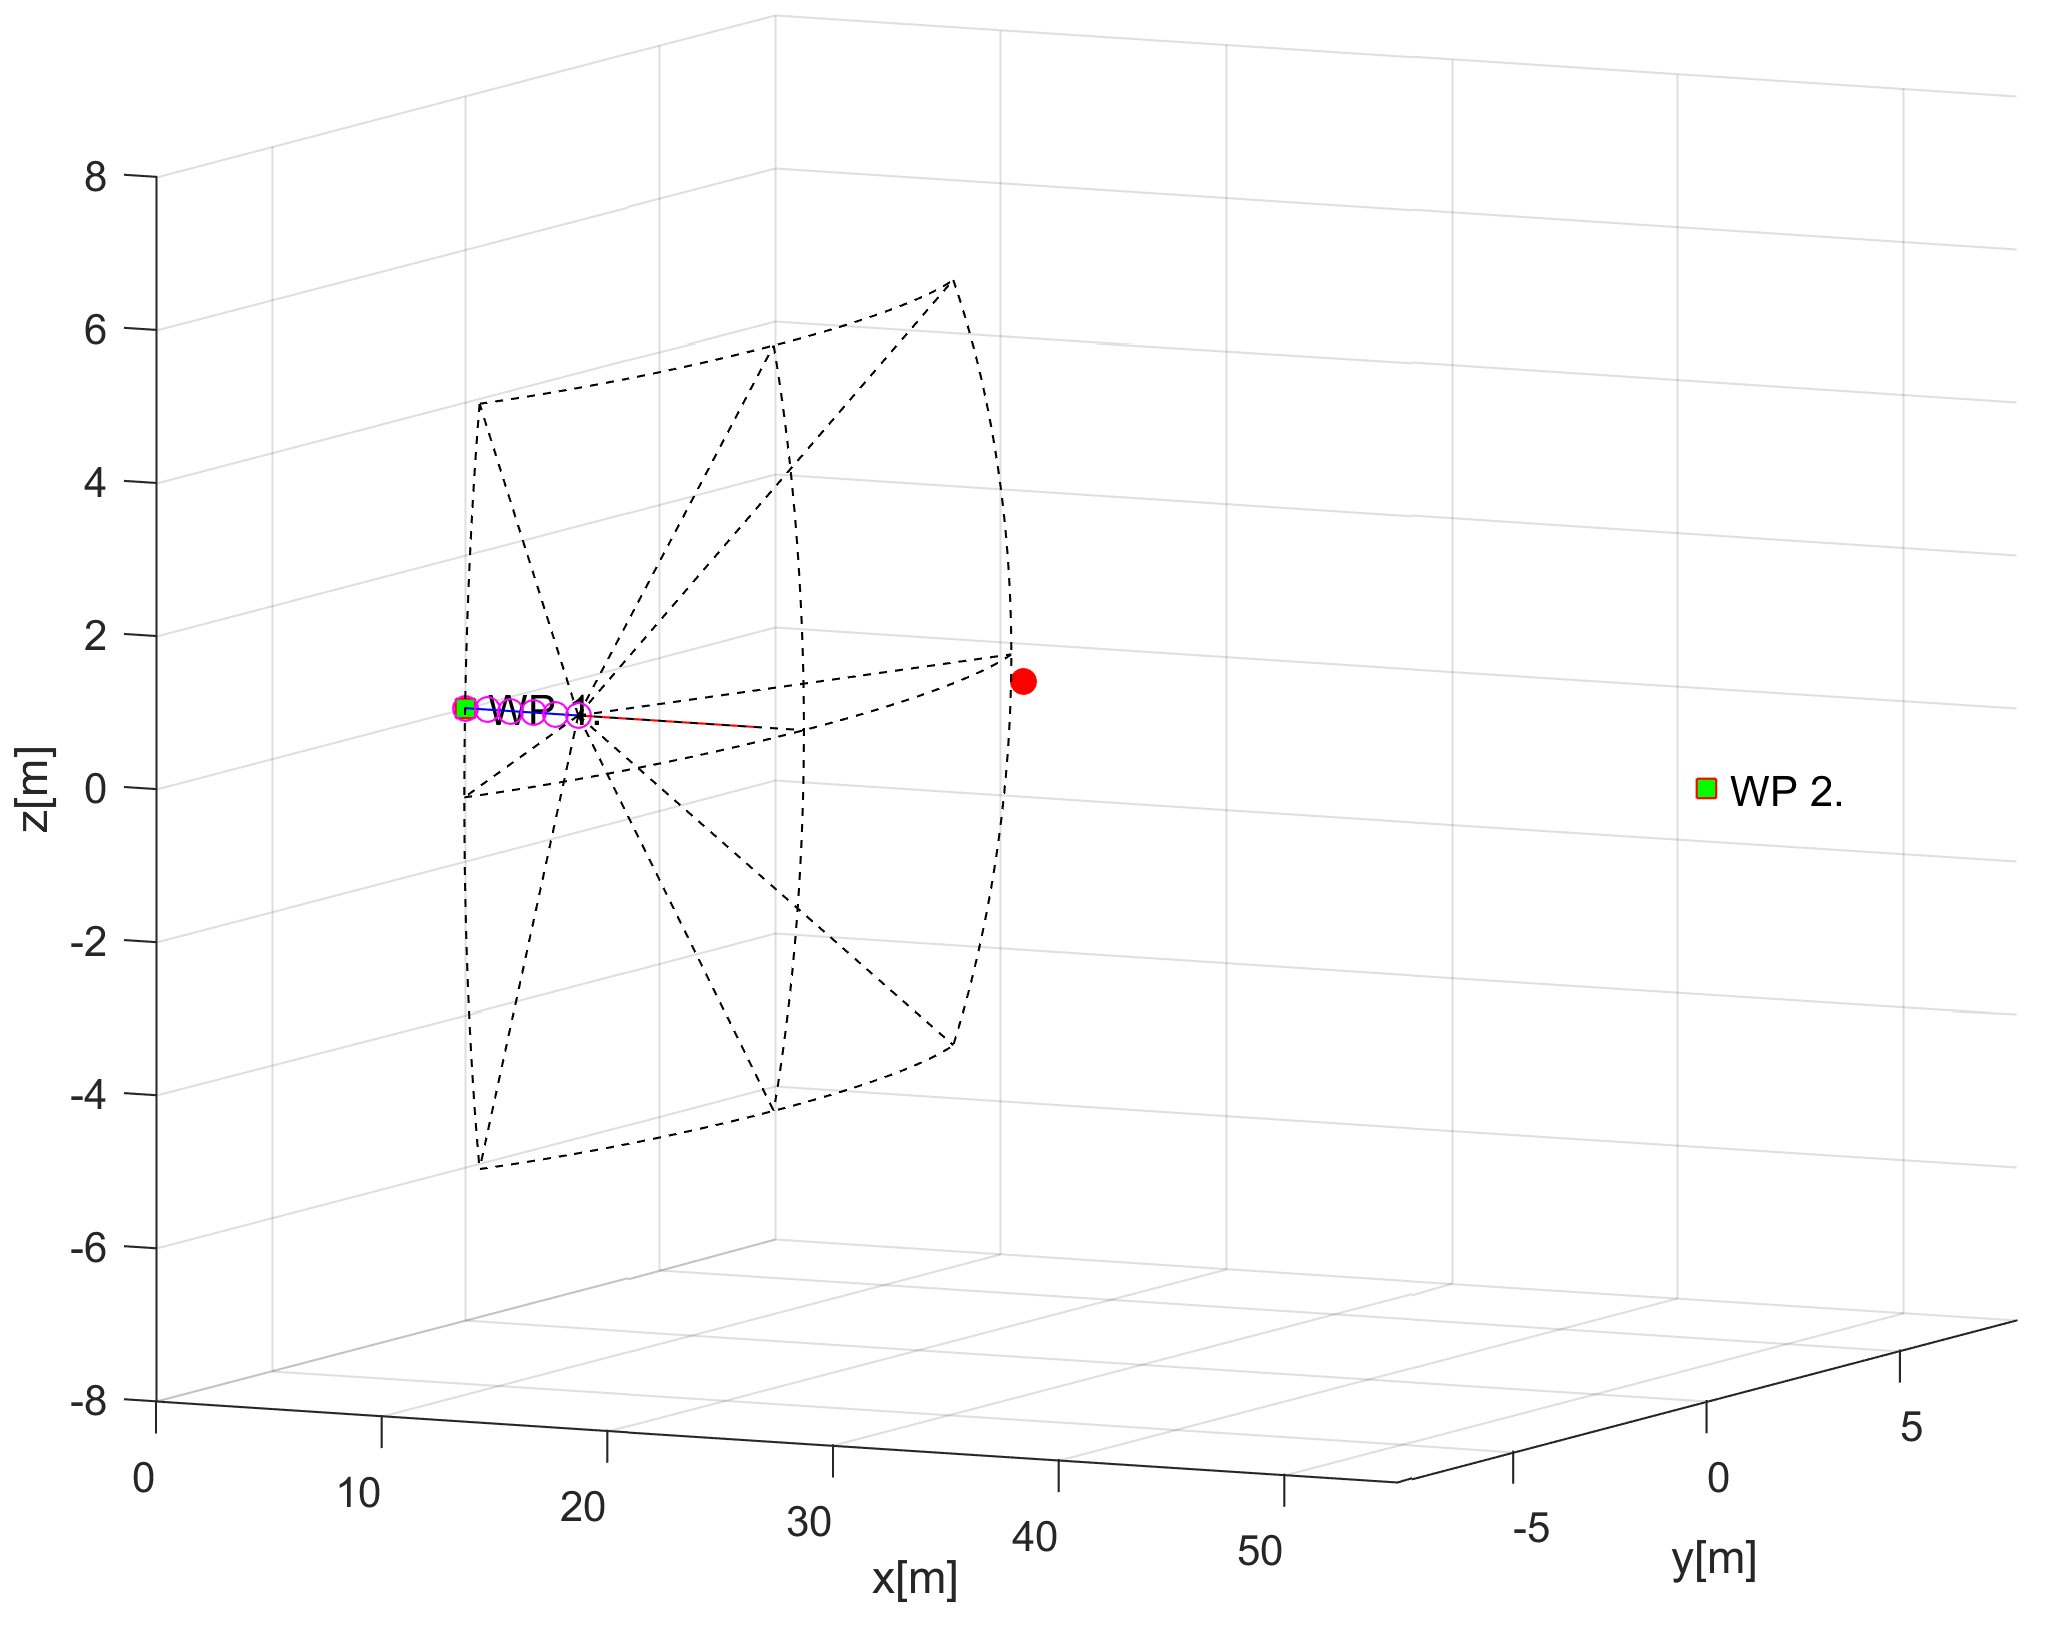
\includegraphics[width=\textwidth]{\FIGDIR/P40FirstIntruderSideHit}
    \caption{First intruder detection.}
    \label{fig:P40FirstIntruderSideHit}
\end{figure}

\noindent\emph{First intruder detection} (fig. \ref{fig:P40FirstIntruderSideHit}) shows intruder $i_1\in\mathscr{I}$ approaching vehicle (defender) from its left flank. It is guaranteed that the intruder $i_1$ and vehicle will clash each other at time $t_i+4s$, if and only if vehicle does not change course. The \emph{vehicle} is also looking for an optimal avoidance trajectory to lower the energy consumption (reminder: simple flew trajectory was used as cost function). 

\begin{figure}[H]
    \centering
    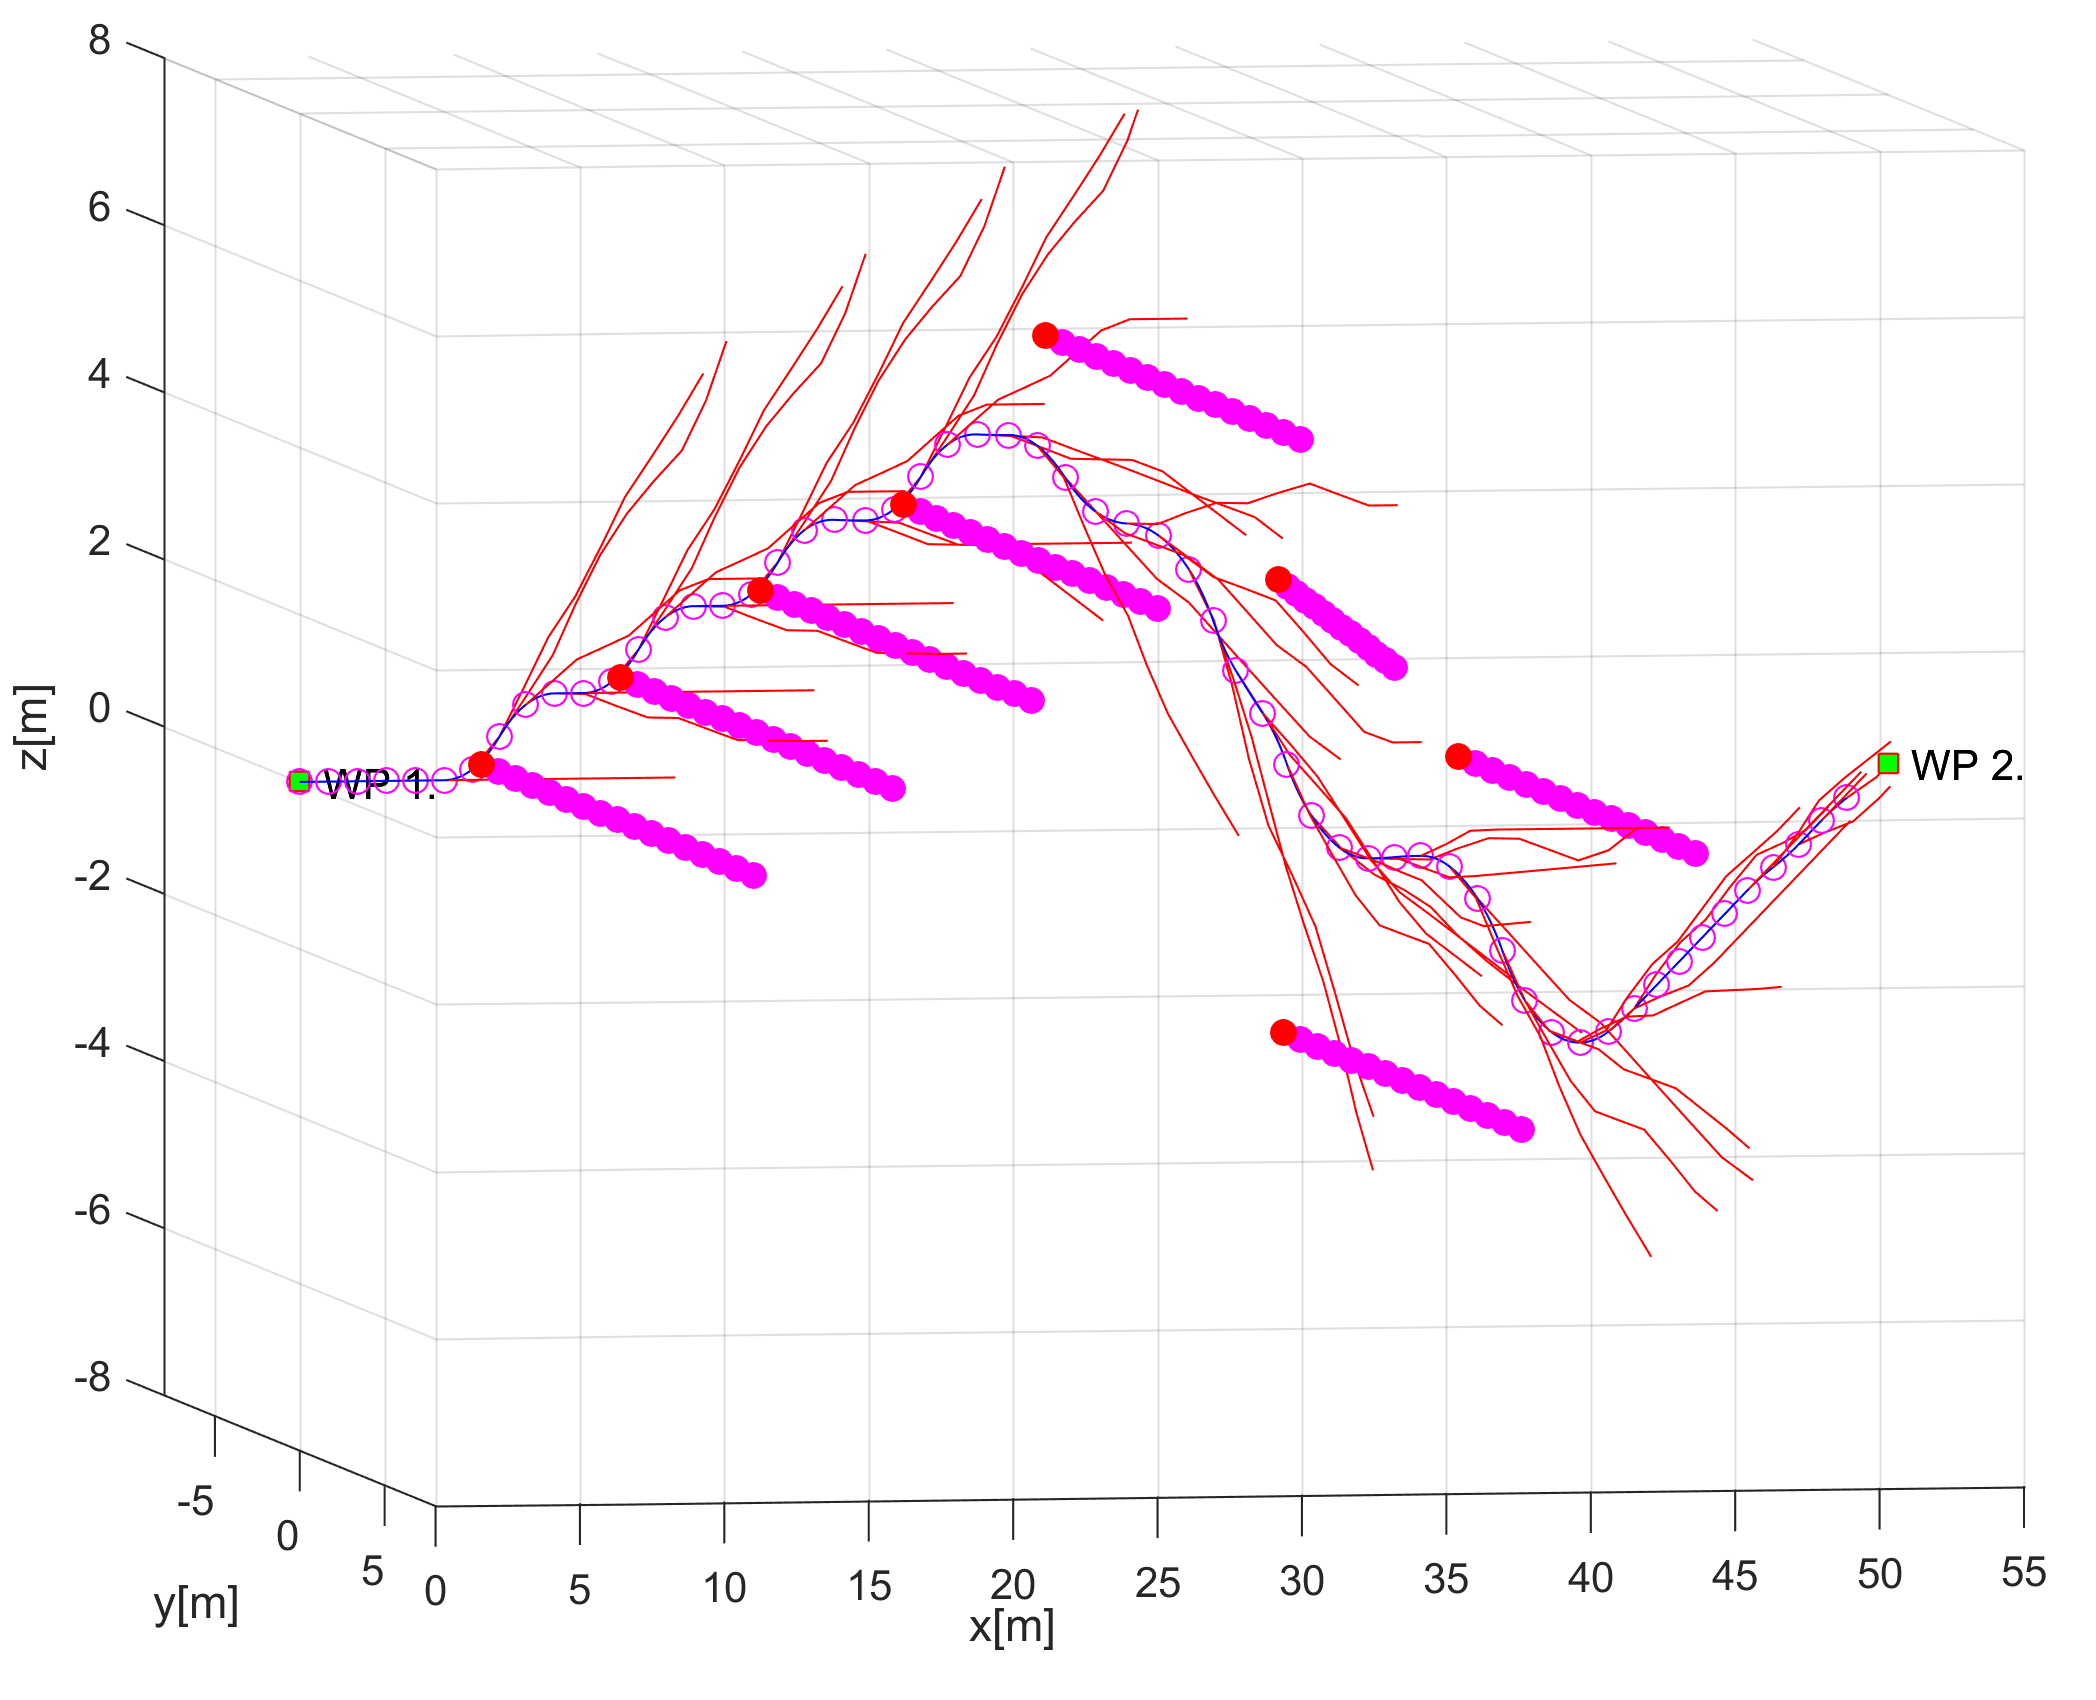
\includegraphics[width=\textwidth]{\FIGDIR/P44IntruderAfterAvoidance}
    \caption{After all intruders avoidance}
    \label{fig:P44IntruderAfterAvoidance}
\end{figure}
\noindent The final trajectory \emph{after all intruder avoidance $i_1,\dots,i_8$} is given by fig.\ref{fig:P44IntruderAfterAvoidance}. Please notice multiple trajectory change given by discovered intruders (tab. \ref{tab:intruderSet}).

\subsection{Intruder avoidance evaluation}
\noindent Due to the best knowledge of authors, all previously discussed conservative/adaptive approaches are mixing together the static and moving obstacles. There is not an single approach which separates concept of static and concept of moving obstacles (intruders) like proposed approach. 

The only important and necessary condition is safety margin, which in this case is given as: 
\begin{equation}
    s_m(i_k) = s_m + 2\times r_i(i_k)
\end{equation}
\noindent Where $s_m$ is safety margin of \emph{our vehicle}, $s_m(i_k)$ is safety margin for selected intruder. The intruder safety margin is depending on intruder body volume, in this case body volume is given by radius $r_i(i_k)$. All intruders $\forall i_k\in\mathscr{I}$ have body radius  $r_i$ equal to $60$ $cm$, therefore the safety margin for any intruder avoidance $s_m(\forall i_k)=1.2 m$.

\begin{figure}[H]
    \centering
    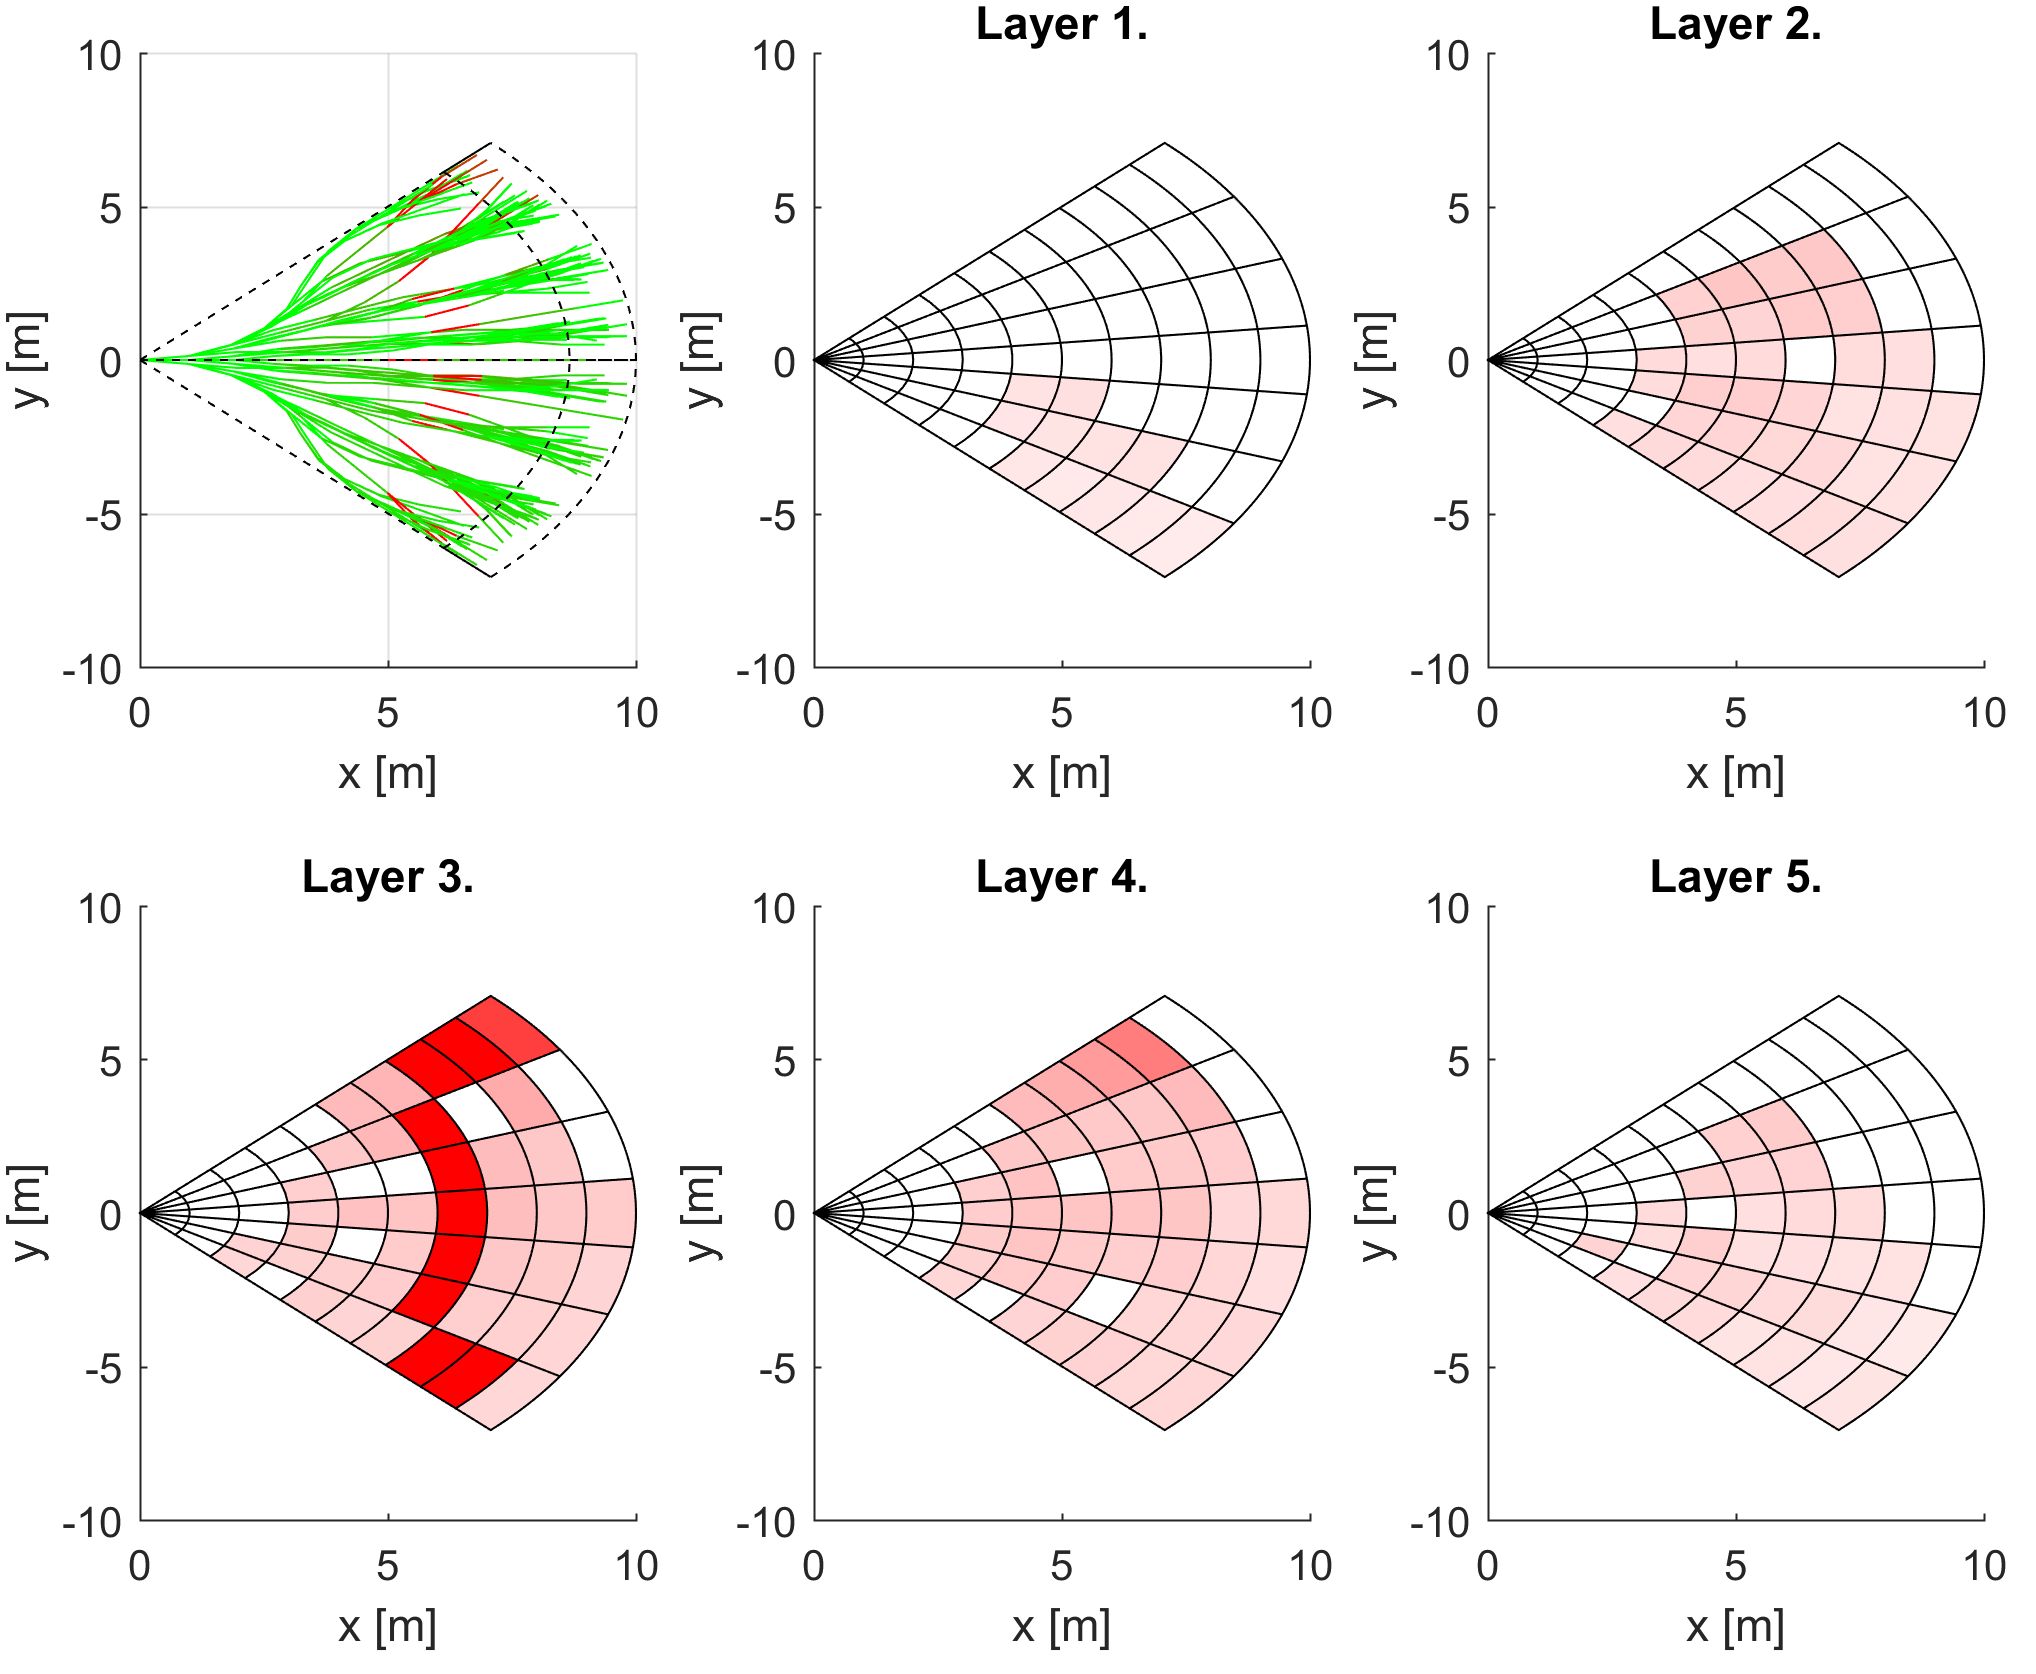
\includegraphics[width=\textwidth]{\FIGDIR/P42IntruderObstacleSpace}
    \caption{Obstacle probability after first intruder detection}
    \label{fig:P42IntruderObstacleSpace}
\end{figure}
\noindent\emph{Obstacle probability} $P_{O_I}$ (fig. \ref{fig:P42IntruderObstacleSpace}) is combination of \emph{linear intersection model} (\ref{eq:baseIntersectionProbabilityLineIntersectionType}) and \emph{conic intersection model} (\ref{eq:spreadIntruderIntersectionProbDiscrete}).

The trajectory set $\{\mathscr{T}\}\in\mathscr{R}$ is given by first sub-figure, only direct intersection cell belonging trajectories are impacted (red). Other trajectories in cones are less impacted (shades of green). 

\emph{Layer 1.} is impacted on right side and its the least impacted layer, due the lowered intruder position $z=-0.5$ ($i_1$ in tab. \ref{tab:intruderSet}). \emph{Layer 2.} contains only residuals from conic intersection and only one row on left side is free for avoidance. \emph{Layer 3.} contains direct line intersection (bright red cells) and residual conic intersection (shades of red) its one of the most impacted layers. \emph{Layer 4.} contains conic intersection residuals (shades of red), almost all layer is covered, but the probabilities of clash are rather low ($\tilde 2.5 \%$). \emph{Layer 5.} contains conic intersection residuals, it is almost symmetrical with layer 2.

\begin{figure}[H]
    \centering
    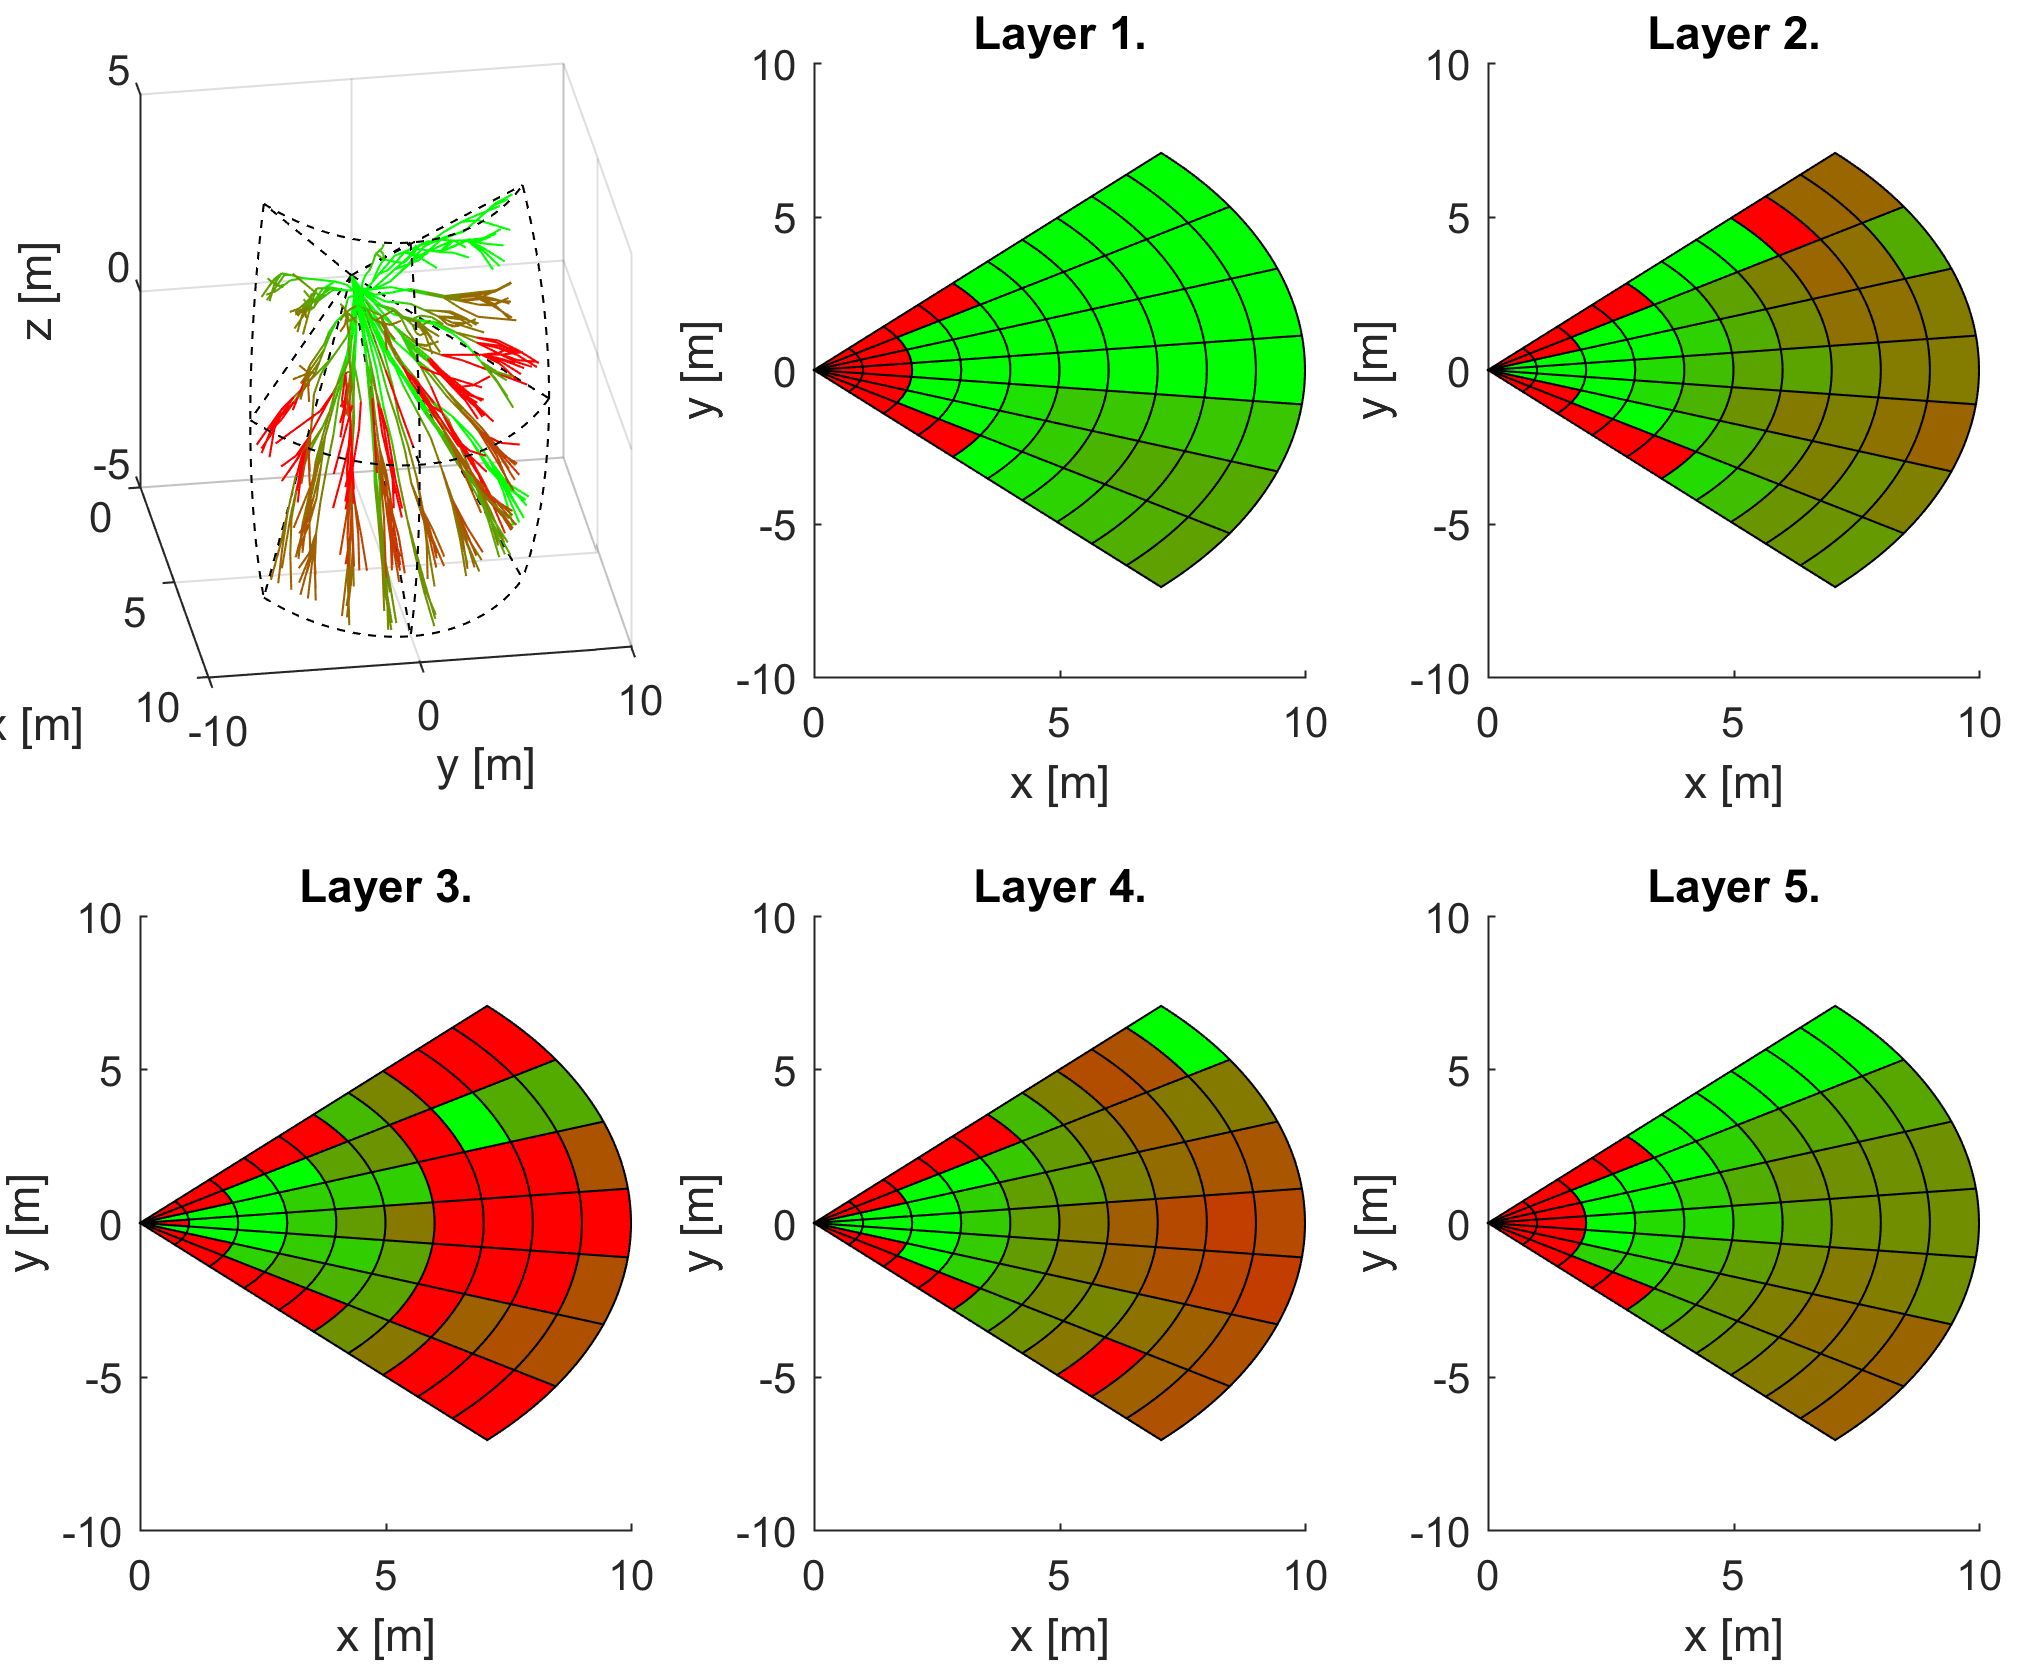
\includegraphics[width=\textwidth]{\FIGDIR/P41IntruderReachiSet}
    \caption{Reachibility probability after first intruder detection}
    \label{fig:P41IntruderReachiSet}
\end{figure}
The reach set $\mathscr{R}(\hat{x}(t_i),t_i,t_{i+1})$ for situation (fig. \ref{fig:P40FirstIntruderSideHit}) is given at top-left sub-figure  (\ref{fig:P41IntruderReachiSet}), the trajectories are colored green if reachable, brownish is semi-reachable, and red if unreachable. Please note that majority of brown trajectories are leading trough layers except intersection one (layer 3).

Reachability probability $P_R(c_{i,j,k})$ for cells $c_{i,j,k}\in\mathscr{A}(t_i)$ is varying due the different distribution of obstacle space (fig. \ref{fig:P42IntruderObstacleSpace}). The green cells are fully reachable, the brownish cells are partially reachable (more red then worse is reachability), the red cells are unreachable. \emph{Layer 1} is reachable in upper half. \emph{Layer 2.} is partially reachable on the edge, due the many routes leading trough safe \emph{layer 1}. \emph{Layer 3.} is completely blocked due the linear part of obstacle intersection ($P_{O_I}=1$). \emph{Layer 4.} is similar to \emph{layer 2.} but there are no patches of reachable space, because \emph{layer 5.} has only one reachable cell row $\mathscr{C}(1,5)$ (\ref{eq:cellrowDefinition}).


\begin{figure}[H]
    \centering
    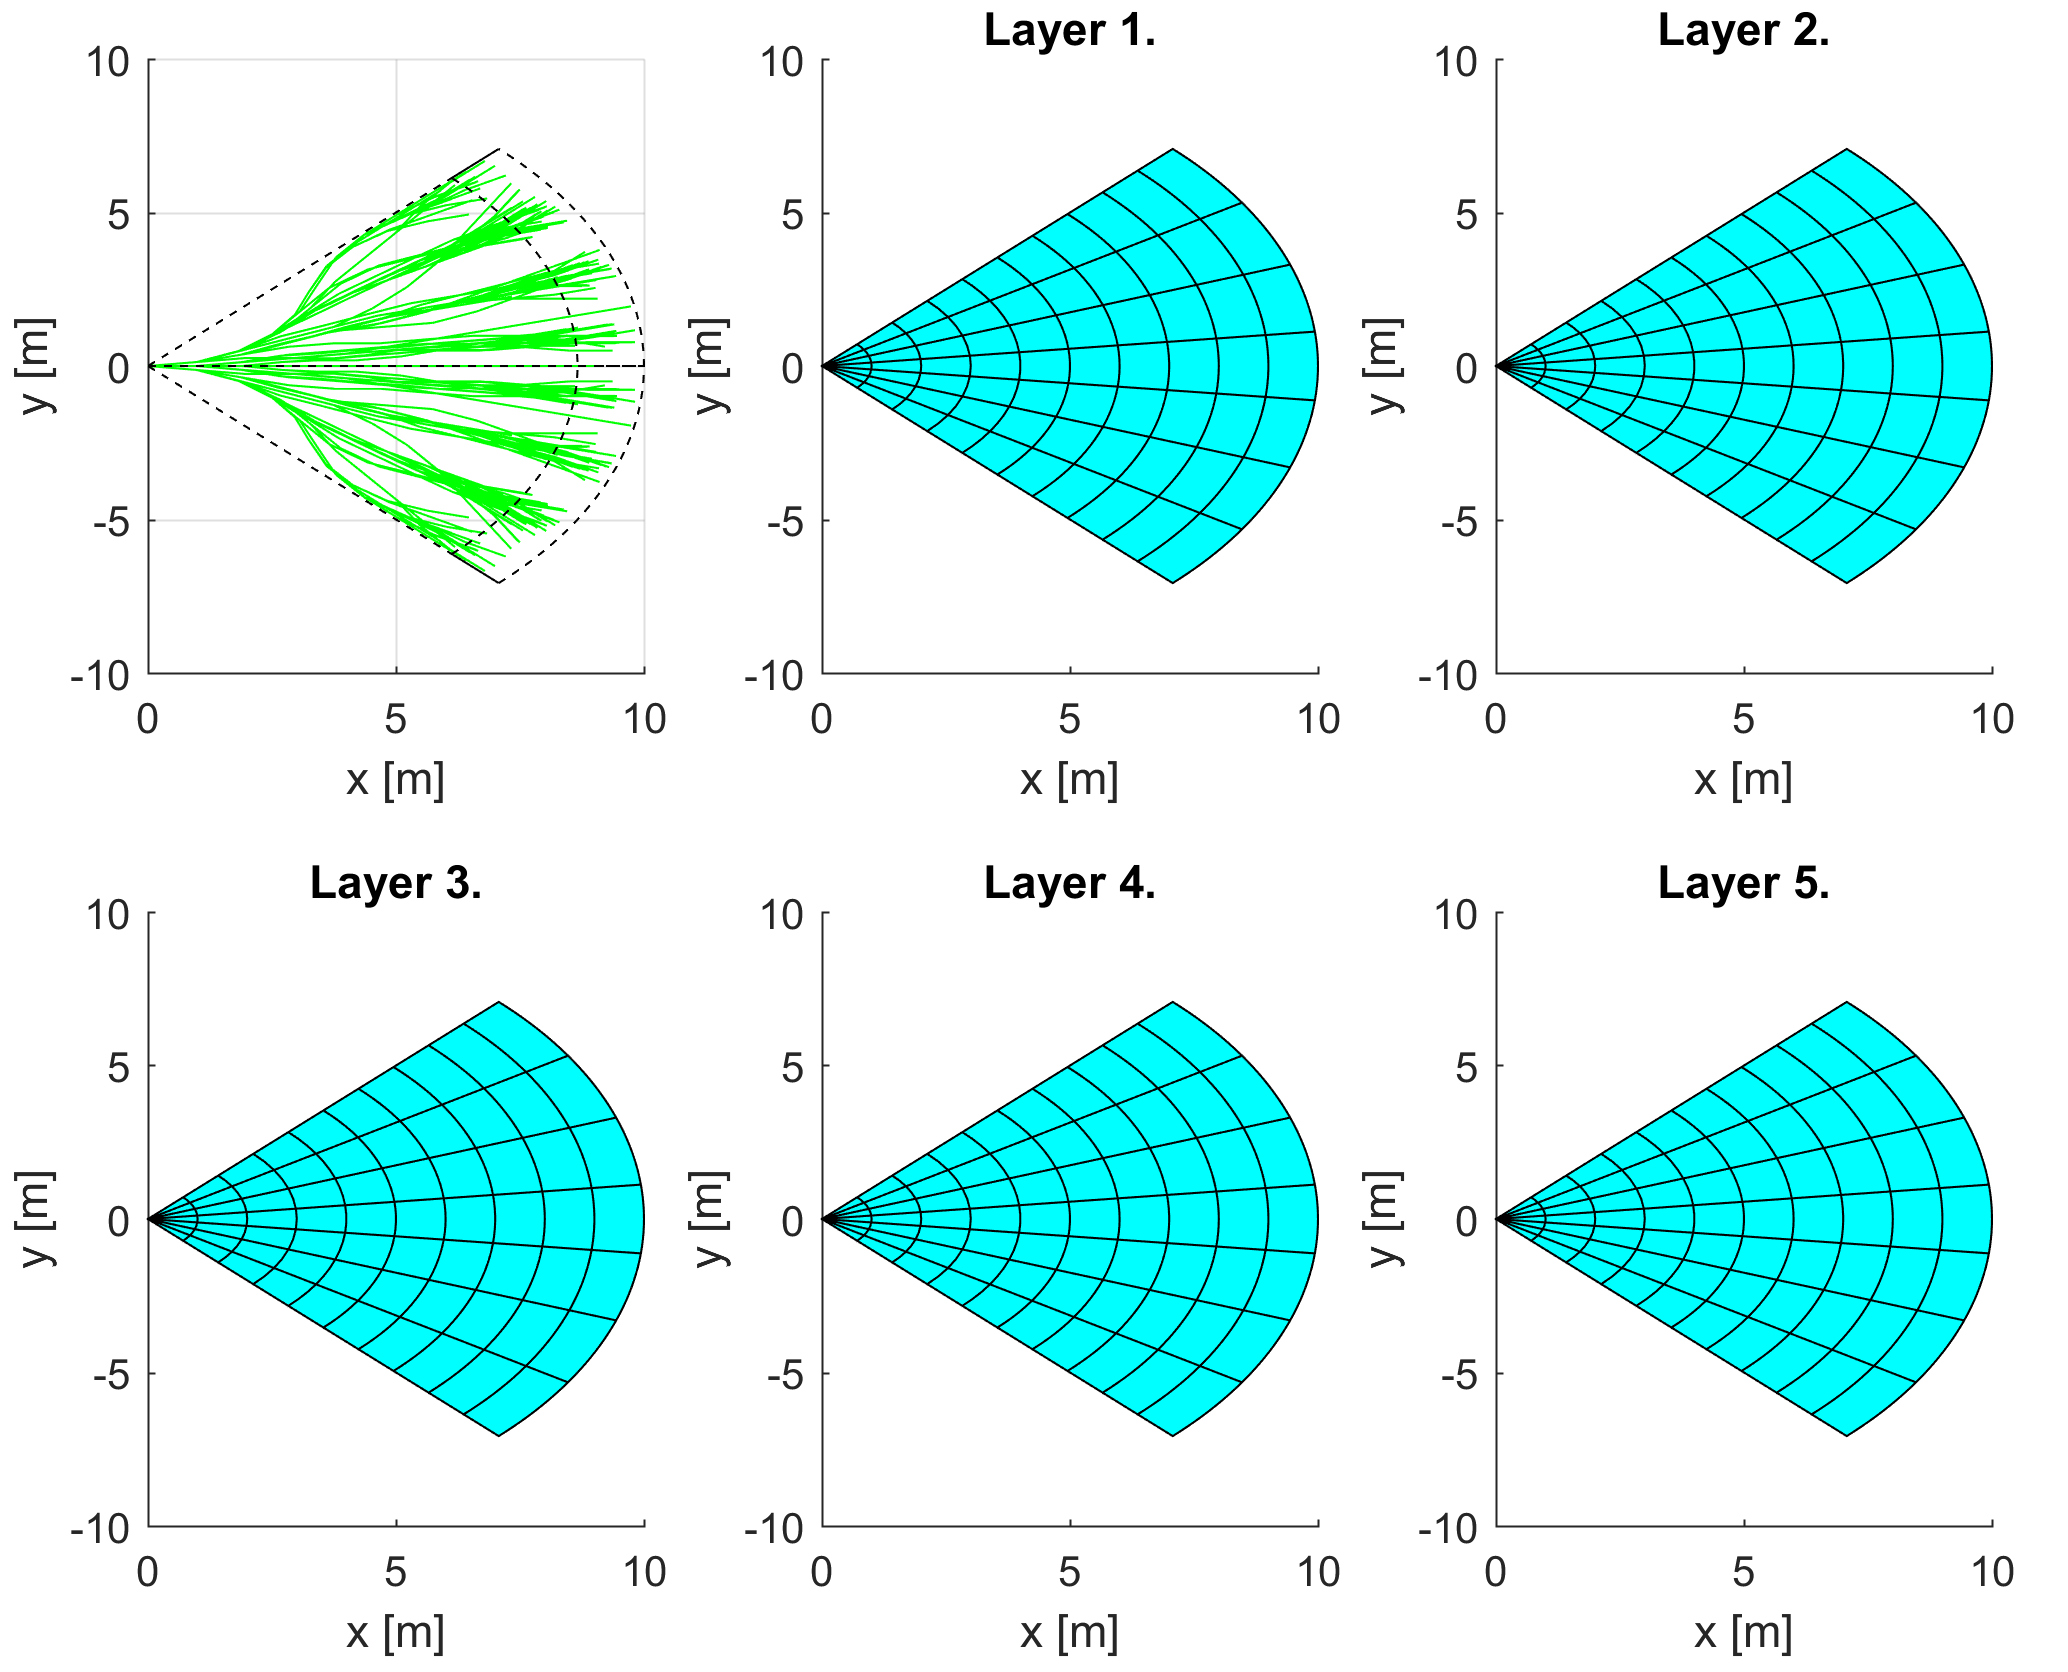
\includegraphics[width=\textwidth]{\FIGDIR/P43IntruderVisibility}
    \caption{Visibility probability after first intruder detection}
    \label{fig:P43IntruderVisibility}
\end{figure}
\noindent The visibility probability $P_V(C_{i,j,k})$ is equal to one for all cells, because there is no real hindrance in visibility. The intruder obstacle probability $P_{O_I}$ can be accounted as a sort of virtual obstacle to be avoided. 

Concept of \emph{virtual obstacles} is very strong and it can be used to implement virtual barriers around object of significant importance.

\emph{Intruder collision distance} $c_D(t)$ is a minimal distance between any intruder and vehicle trajectory at given time snapshot $\tau$. For fixed time $\tau$, there exist a set of intruder positions like follow:
\begin{equation}\label{eq:setOfIntrudersPositionsFixedTime}
    \mathscr{I}_P(\tau)=\left\{\vec{p}\in\R^3:p=\vec{x}(\tau)\to\R^3,\vec{x}(\tau)\in i_k, i_k\in \mathscr{I}(\tau)\right\}
\end{equation}
Where $\vec{p}$ is point in global coordinates, created by projection of intruder state $\vec{x}(\tau)$ to \emph{global coordinate frame} $\R^3$ for each intruder $i_k$ in detected intruders set $\mathscr{I}(\tau)$.

\emph{The closest intruder} $i_c$ in detected intruder set $\mathscr{I}(\tau)$ for fixed time $\tau$ is given as:
\begin{equation}
    i_c(\tau,\vec{x}_v(\tau))=i_k\in\mathscr{I}:\min_{\forall \vec{p}_i\in\mathscr{I}_P(\tau), \vec{x}_v(\tau)}\left\{\norm{\vec{p}_i-\left( \vec{x}_v(\tau)\to\R^3\right)}\right\}
\end{equation}
Where the $\vec{x}_v(\tau)\to\R^3$ is projection of our vehicle state $\vec{x}_v$ at fixed time $\tau$ projected to global coordinate frame $\mathscr{R}^3$, the closest intruder $i_c$ is selected based on vehicle position and set of intruders positions $\mathscr{I}_P(\tau)$ (\ref{eq:setOfIntrudersPositionsFixedTime}). The norm $\norm{\cdot}$ is standard euclidean. 

\emph{Collision distance} function $c_D(t)$ is calculated for steepest time $\tau$ in mission time frame $[t_s,t_e]$, where $t_s$ is mission start time and $t_e$ mission end time. For fixed time $\tau$ the minimal distance between vehicle position $\vec{x}_v(\tau)\to\R^3$ in global coordinate frame $\R^3$, and intruder position $\vec{p}_i$ from intruder set $\mathscr{I}_P(\tau)$ used as crash distance $c_d$ for particular $\tau$. The collision distance is formulated in following equation:
\begin{equation}
    c_D(t)=\left\{c_d\in\R: c_d=\min_{\forall \vec{p}_i\in\mathscr{I}_P(\tau), \vec{x}_v(\tau)}\left\{\norm{\vec{p}_i-\left( \vec{x}_v(\tau)\to\R^3\right)}\right\}, \forall \tau \in [t_s,t_e]\right\}
\end{equation}

\begin{figure}[H]
    \centering
    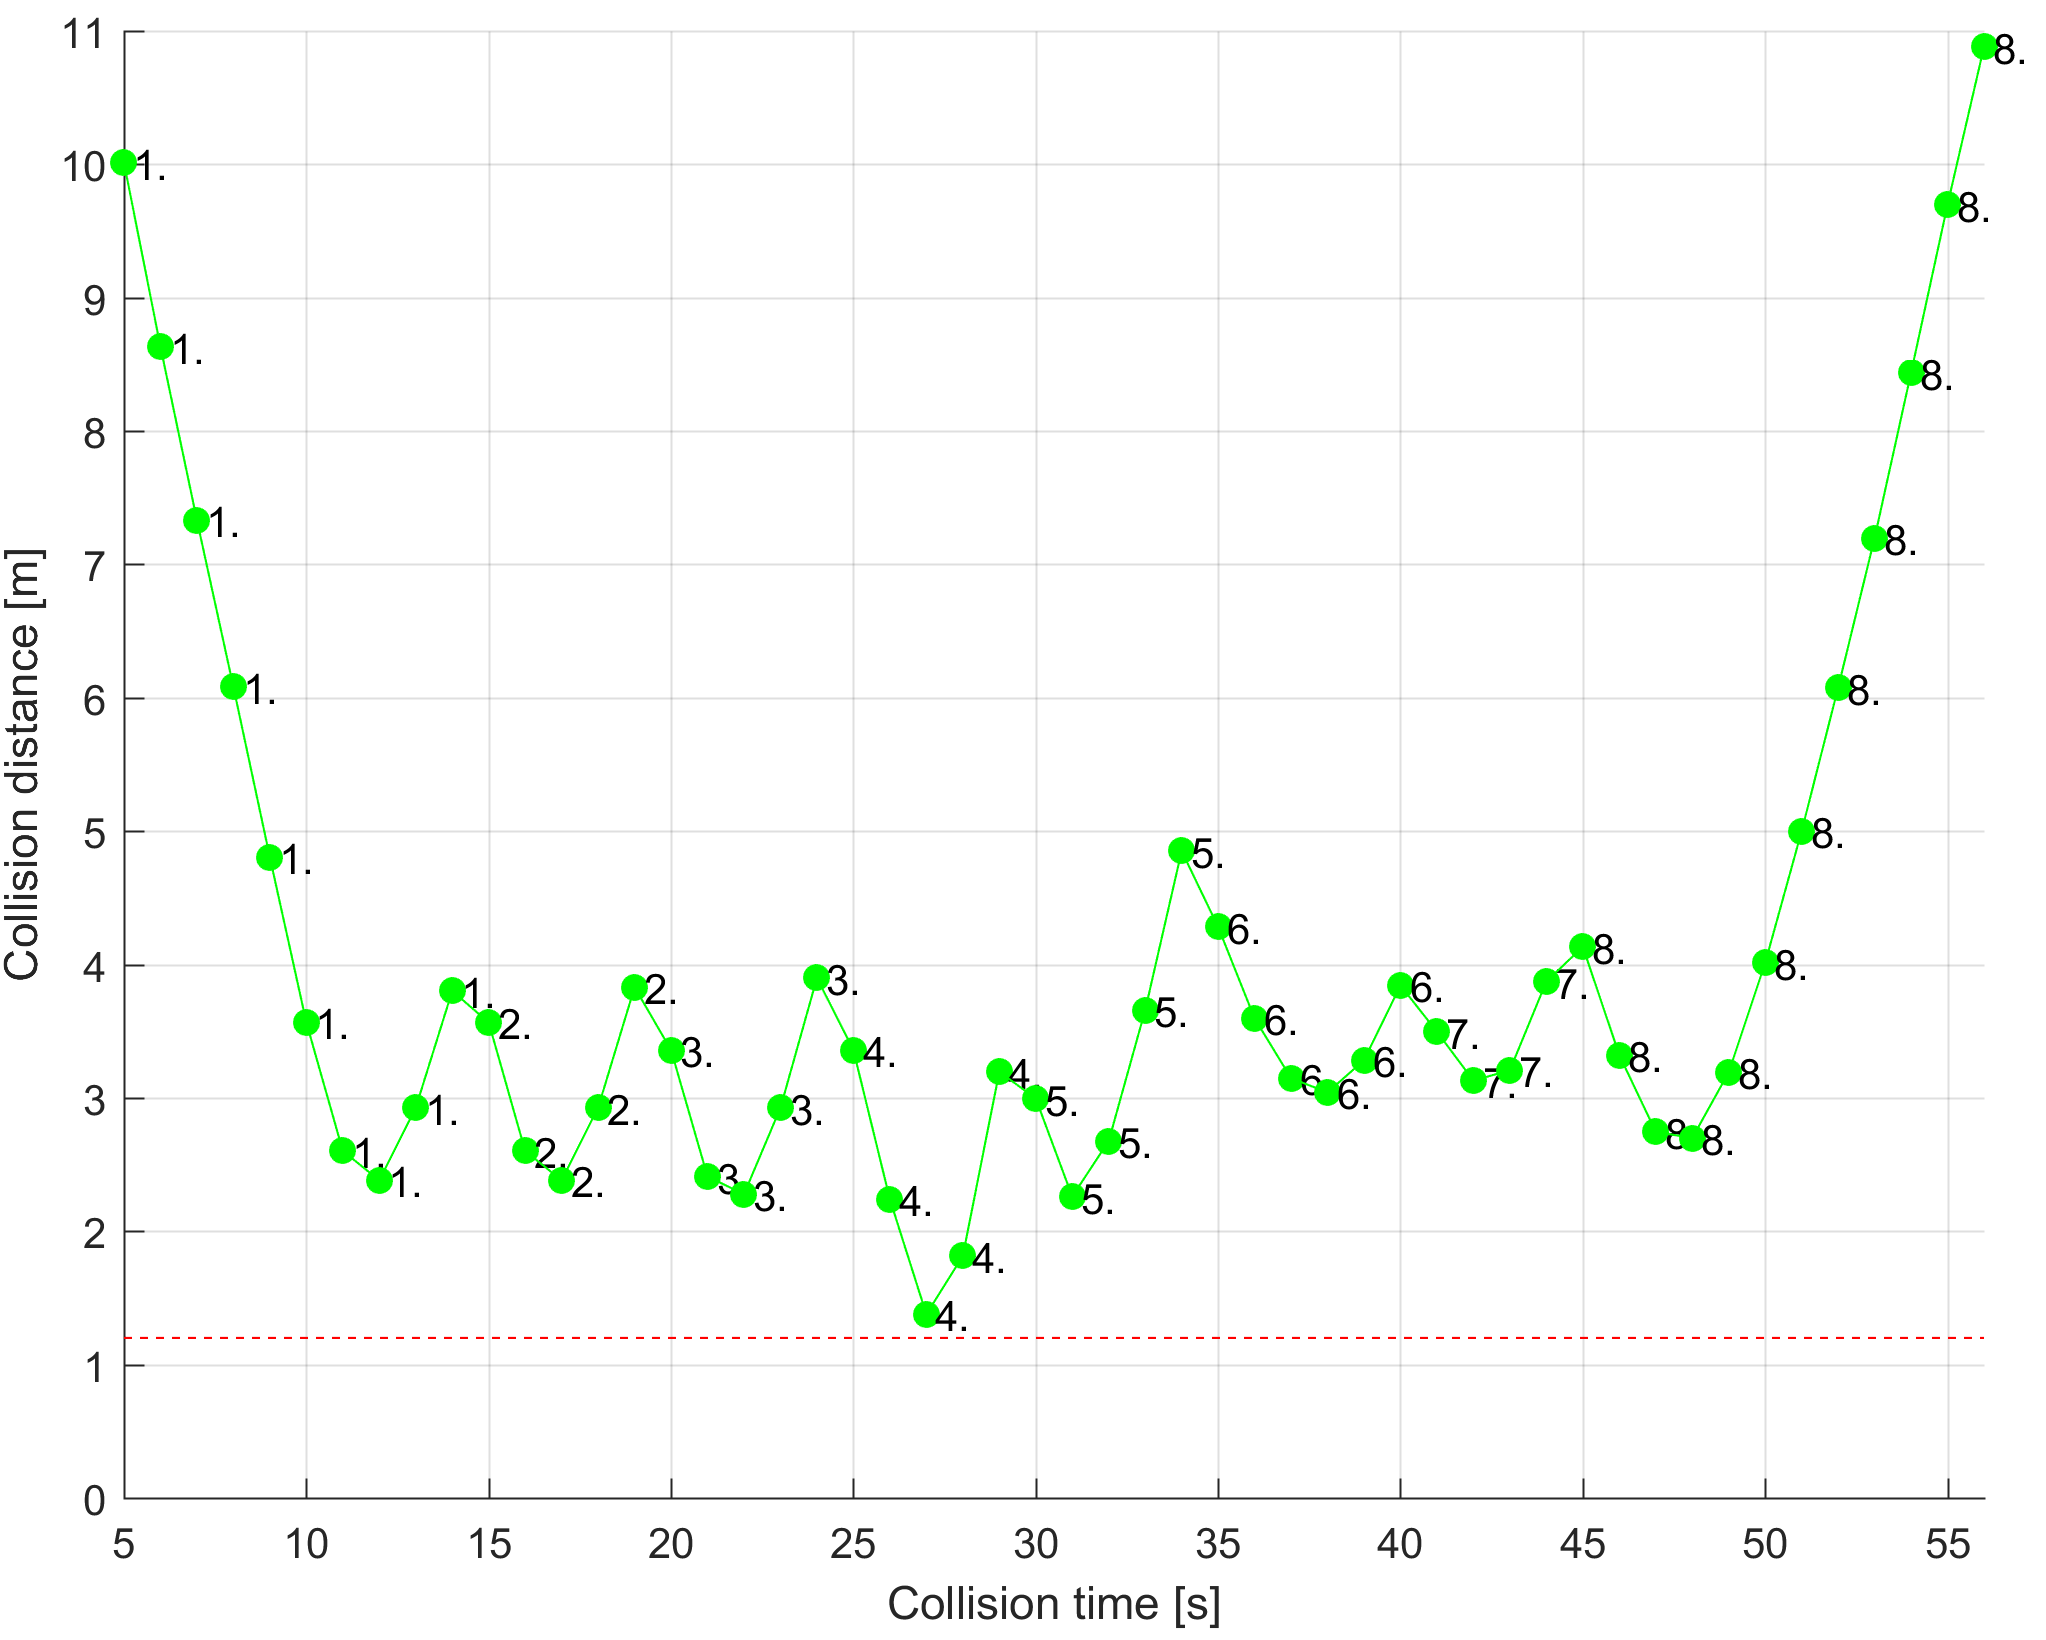
\includegraphics[width=\textwidth]{\FIGDIR/P45IntruderDistanceEvolution}
    \caption{Intruder collision distance $c_d(t)$ evolution.}
    \label{fig:P45IntruderDistanceEvolution}
\end{figure}

\noindent \emph{Intruder collision distance $c_d(t)$ evolution} (\ref{fig:P45IntruderDistanceEvolution}) shows that the necessary condition $c_D(t)\ge s_m (1.2 m)$ holds. \emph{Green line} shows evolution over time. \emph{Green full circles} are marking the closest intruder $i_k\in\mathscr{I}(t)$, defined in table \ref{tab:intruderSet}. The time starts at $5s$ when first intruder is detected. The evolution of $c_D(t)$ reflects how intruders were popping out and tried to collide with our vehicle. The closest intruder was $i_4$ whom achieves distance of $136 cm$.
